\documentclass[twoside]{book}

% Packages required by doxygen
\usepackage{calc}
\usepackage{doxygen}
\usepackage{graphicx}
\usepackage[utf8]{inputenc}
\usepackage{makeidx}
\usepackage{multicol}
\usepackage{multirow}
\usepackage{textcomp}
\usepackage[table]{xcolor}

% Font selection
\usepackage[T1]{fontenc}
\usepackage{mathptmx}
\usepackage[scaled=.90]{helvet}
\usepackage{courier}
\usepackage{amssymb}
\usepackage{sectsty}
\renewcommand{\familydefault}{\sfdefault}
\allsectionsfont{%
  \fontseries{bc}\selectfont%
  \color{darkgray}%
}
\renewcommand{\DoxyLabelFont}{%
  \fontseries{bc}\selectfont%
  \color{darkgray}%
}

% Page & text layout
\usepackage{geometry}
\geometry{%
  a4paper,%
  top=2.5cm,%
  bottom=2.5cm,%
  left=2.5cm,%
  right=2.5cm%
}
\tolerance=750
\hfuzz=15pt
\hbadness=750
\setlength{\emergencystretch}{15pt}
\setlength{\parindent}{0cm}
\setlength{\parskip}{0.2cm}
\makeatletter
\renewcommand{\paragraph}{%
  \@startsection{paragraph}{4}{0ex}{-1.0ex}{1.0ex}{%
    \normalfont\normalsize\bfseries\SS@parafont%
  }%
}
\renewcommand{\subparagraph}{%
  \@startsection{subparagraph}{5}{0ex}{-1.0ex}{1.0ex}{%
    \normalfont\normalsize\bfseries\SS@subparafont%
  }%
}
\makeatother

% Headers & footers
\usepackage{fancyhdr}
\pagestyle{fancyplain}
\fancyhead[LE]{\fancyplain{}{\bfseries\thepage}}
\fancyhead[CE]{\fancyplain{}{}}
\fancyhead[RE]{\fancyplain{}{\bfseries\leftmark}}
\fancyhead[LO]{\fancyplain{}{\bfseries\rightmark}}
\fancyhead[CO]{\fancyplain{}{}}
\fancyhead[RO]{\fancyplain{}{\bfseries\thepage}}
\fancyfoot[LE]{\fancyplain{}{}}
\fancyfoot[CE]{\fancyplain{}{}}
\fancyfoot[RE]{\fancyplain{}{\bfseries\scriptsize Generated on Thu May 2 2019 15\-:28\-:32 for Snoke by Doxygen }}
\fancyfoot[LO]{\fancyplain{}{\bfseries\scriptsize Generated on Thu May 2 2019 15\-:28\-:32 for Snoke by Doxygen }}
\fancyfoot[CO]{\fancyplain{}{}}
\fancyfoot[RO]{\fancyplain{}{}}
\renewcommand{\footrulewidth}{0.4pt}
\renewcommand{\chaptermark}[1]{%
  \markboth{#1}{}%
}
\renewcommand{\sectionmark}[1]{%
  \markright{\thesection\ #1}%
}

% Indices & bibliography
\usepackage{natbib}
\usepackage[titles]{tocloft}
\setcounter{tocdepth}{3}
\setcounter{secnumdepth}{5}
\makeindex

% Hyperlinks (required, but should be loaded last)
\usepackage{ifpdf}
\ifpdf
  \usepackage[pdftex,pagebackref=true]{hyperref}
\else
  \usepackage[ps2pdf,pagebackref=true]{hyperref}
\fi
\hypersetup{%
  colorlinks=true,%
  linkcolor=blue,%
  citecolor=blue,%
  unicode%
}

% Custom commands
\newcommand{\clearemptydoublepage}{%
  \newpage{\pagestyle{empty}\cleardoublepage}%
}


%===== C O N T E N T S =====

\begin{document}

% Titlepage & ToC
\hypersetup{pageanchor=false}
\pagenumbering{roman}
\begin{titlepage}
\vspace*{7cm}
\begin{center}%
{\Large Snoke }\\
\vspace*{1cm}
{\large Generated by Doxygen 1.8.6}\\
\vspace*{0.5cm}
{\small Thu May 2 2019 15:28:32}\\
\end{center}
\end{titlepage}
\clearemptydoublepage
\tableofcontents
\clearemptydoublepage
\pagenumbering{arabic}
\hypersetup{pageanchor=true}

%--- Begin generated contents ---
\chapter{What is Snoke?}
\label{md__home_travis_build_echo-team__snoke__r_e_a_d_m_e}
\hypertarget{md__home_travis_build_echo-team__snoke__r_e_a_d_m_e}{}
An extended version of the console game called \char`\"{}\-Snake\char`\"{}. \paragraph*{Warm memories}

This game will provide you a lot of oldschool fun and nostalgy. Collect your friends, create a team and fight another teams and organisations. \paragraph*{Justice}

Shoke is a new way of solving argues. Just stand the idea and see how many people are ready to defend it! \paragraph*{Arcade}

Designed for people who trying to cope with waiting. Play the arcade mod while your npm installing packs! 
\chapter{Hierarchical Index}
\section{Class Hierarchy}
This inheritance list is sorted roughly, but not completely, alphabetically\+:\begin{DoxyCompactList}
\item \contentsline{section}{\+\_\+\+Point}{\pageref{struct___point}}{}
\item \contentsline{section}{\+\_\+\+Point\+Style}{\pageref{struct___point_style}}{}
\item \contentsline{section}{Ball}{\pageref{class_ball}}{}
\item \contentsline{section}{Game}{\pageref{class_game}}{}
\item \contentsline{section}{Labyrinth}{\pageref{class_labyrinth}}{}
\item \contentsline{section}{Logo}{\pageref{class_logo}}{}
\item \contentsline{section}{Main\+Menu}{\pageref{class_main_menu}}{}
\item \contentsline{section}{Menu\+Button}{\pageref{struct_menu_button}}{}
\item \contentsline{section}{Navigate\+Unit}{\pageref{struct_navigate_unit}}{}
\item \contentsline{section}{Navigator}{\pageref{class_navigator}}{}
\item \contentsline{section}{Side\+Button}{\pageref{struct_side_button}}{}
\item \contentsline{section}{Side\+Menu}{\pageref{class_side_menu}}{}
\item \contentsline{section}{Snake}{\pageref{class_snake}}{}
\item \contentsline{section}{Widget}{\pageref{class_widget}}{}
\begin{DoxyCompactList}
\item \contentsline{section}{Menu}{\pageref{class_menu}}{}
\end{DoxyCompactList}
\end{DoxyCompactList}

\chapter{Class Index}
\section{Class List}
Here are the classes, structs, unions and interfaces with brief descriptions\-:\begin{DoxyCompactList}
\item\contentsline{section}{\hyperlink{struct___point}{\-\_\-\-Point} }{\pageref{struct___point}}{}
\item\contentsline{section}{\hyperlink{struct___point_style}{\-\_\-\-Point\-Style} }{\pageref{struct___point_style}}{}
\item\contentsline{section}{\hyperlink{class_ball}{Ball} }{\pageref{class_ball}}{}
\item\contentsline{section}{\hyperlink{class_game}{Game} }{\pageref{class_game}}{}
\item\contentsline{section}{\hyperlink{class_labyrinth}{Labyrinth} }{\pageref{class_labyrinth}}{}
\item\contentsline{section}{\hyperlink{class_logo}{Logo} }{\pageref{class_logo}}{}
\item\contentsline{section}{\hyperlink{class_main_menu}{Main\-Menu} }{\pageref{class_main_menu}}{}
\item\contentsline{section}{\hyperlink{class_menu}{Menu} }{\pageref{class_menu}}{}
\item\contentsline{section}{\hyperlink{struct_menu_button}{Menu\-Button} }{\pageref{struct_menu_button}}{}
\item\contentsline{section}{\hyperlink{struct_navigate_unit}{Navigate\-Unit} }{\pageref{struct_navigate_unit}}{}
\item\contentsline{section}{\hyperlink{class_navigator}{Navigator} }{\pageref{class_navigator}}{}
\item\contentsline{section}{\hyperlink{struct_side_button}{Side\-Button} }{\pageref{struct_side_button}}{}
\item\contentsline{section}{\hyperlink{class_side_menu}{Side\-Menu} }{\pageref{class_side_menu}}{}
\item\contentsline{section}{\hyperlink{class_snake}{Snake} }{\pageref{class_snake}}{}
\item\contentsline{section}{\hyperlink{class_widget}{Widget} }{\pageref{class_widget}}{}
\end{DoxyCompactList}

\chapter{File Index}
\section{File List}
Here is a list of all files with brief descriptions\-:\begin{DoxyCompactList}
\item\contentsline{section}{/home/travis/build/echo-\/team/\-Snoke/\hyperlink{_main_8cpp}{Main.\-cpp} }{\pageref{_main_8cpp}}{}
\item\contentsline{section}{/home/travis/build/echo-\/team/\-Snoke/\-Libraries/\-Ball/\hyperlink{ball_8cpp}{ball.\-cpp} }{\pageref{ball_8cpp}}{}
\item\contentsline{section}{/home/travis/build/echo-\/team/\-Snoke/\-Libraries/\-Ball/\hyperlink{ball_8h}{ball.\-h} }{\pageref{ball_8h}}{}
\item\contentsline{section}{/home/travis/build/echo-\/team/\-Snoke/\-Libraries/\-Common/\hyperlink{common_8cpp}{common.\-cpp} }{\pageref{common_8cpp}}{}
\item\contentsline{section}{/home/travis/build/echo-\/team/\-Snoke/\-Libraries/\-Common/\hyperlink{common_8h}{common.\-h} }{\pageref{common_8h}}{}
\item\contentsline{section}{/home/travis/build/echo-\/team/\-Snoke/\-Libraries/\-Game/\hyperlink{game_8cpp}{game.\-cpp} }{\pageref{game_8cpp}}{}
\item\contentsline{section}{/home/travis/build/echo-\/team/\-Snoke/\-Libraries/\-Game/\hyperlink{game_8h}{game.\-h} }{\pageref{game_8h}}{}
\item\contentsline{section}{/home/travis/build/echo-\/team/\-Snoke/\-Libraries/\-Interface/\hyperlink{interface_8cpp}{interface.\-cpp} }{\pageref{interface_8cpp}}{}
\item\contentsline{section}{/home/travis/build/echo-\/team/\-Snoke/\-Libraries/\-Interface/\hyperlink{interface_8h}{interface.\-h} }{\pageref{interface_8h}}{}
\item\contentsline{section}{/home/travis/build/echo-\/team/\-Snoke/\-Libraries/\-Interface/\hyperlink{logo_8cpp}{logo.\-cpp} }{\pageref{logo_8cpp}}{}
\item\contentsline{section}{/home/travis/build/echo-\/team/\-Snoke/\-Libraries/\-Interface/\hyperlink{logo_8h}{logo.\-h} }{\pageref{logo_8h}}{}
\item\contentsline{section}{/home/travis/build/echo-\/team/\-Snoke/\-Libraries/\-Interface/\hyperlink{menu_8cpp}{menu.\-cpp} }{\pageref{menu_8cpp}}{}
\item\contentsline{section}{/home/travis/build/echo-\/team/\-Snoke/\-Libraries/\-Interface/\hyperlink{menu_8h}{menu.\-h} }{\pageref{menu_8h}}{}
\item\contentsline{section}{/home/travis/build/echo-\/team/\-Snoke/\-Libraries/\-Interface/\hyperlink{navigator_8cpp}{navigator.\-cpp} }{\pageref{navigator_8cpp}}{}
\item\contentsline{section}{/home/travis/build/echo-\/team/\-Snoke/\-Libraries/\-Interface/\hyperlink{navigator_8h}{navigator.\-h} }{\pageref{navigator_8h}}{}
\item\contentsline{section}{/home/travis/build/echo-\/team/\-Snoke/\-Libraries/\-Labyrinth/\hyperlink{labyrinth_8cpp}{labyrinth.\-cpp} }{\pageref{labyrinth_8cpp}}{}
\item\contentsline{section}{/home/travis/build/echo-\/team/\-Snoke/\-Libraries/\-Labyrinth/\hyperlink{labyrinth_8h}{labyrinth.\-h} }{\pageref{labyrinth_8h}}{}
\item\contentsline{section}{/home/travis/build/echo-\/team/\-Snoke/\-Libraries/\-Screens/\hyperlink{main_menu_8cpp}{main\-Menu.\-cpp} }{\pageref{main_menu_8cpp}}{}
\item\contentsline{section}{/home/travis/build/echo-\/team/\-Snoke/\-Libraries/\-Screens/\hyperlink{main_menu_8h}{main\-Menu.\-h} }{\pageref{main_menu_8h}}{}
\item\contentsline{section}{/home/travis/build/echo-\/team/\-Snoke/\-Libraries/\-Side\-Menu/\hyperlink{_side_menu_8cpp}{Side\-Menu.\-cpp} }{\pageref{_side_menu_8cpp}}{}
\item\contentsline{section}{/home/travis/build/echo-\/team/\-Snoke/\-Libraries/\-Side\-Menu/\hyperlink{_side_menu_8h}{Side\-Menu.\-h} }{\pageref{_side_menu_8h}}{}
\item\contentsline{section}{/home/travis/build/echo-\/team/\-Snoke/\-Libraries/\-Snake/\hyperlink{snake_8cpp}{snake.\-cpp} }{\pageref{snake_8cpp}}{}
\item\contentsline{section}{/home/travis/build/echo-\/team/\-Snoke/\-Libraries/\-Snake/\hyperlink{snake_8h}{snake.\-h} }{\pageref{snake_8h}}{}
\end{DoxyCompactList}

\chapter{Class Documentation}
\hypertarget{struct___point}{}\section{\+\_\+\+Point Struct Reference}
\label{struct___point}\index{\_Point@{\_Point}}


{\ttfamily \#include $<$common.\+h$>$}



Collaboration diagram for \+\_\+\+Point\+:
\nopagebreak
\begin{figure}[H]
\begin{center}
\leavevmode
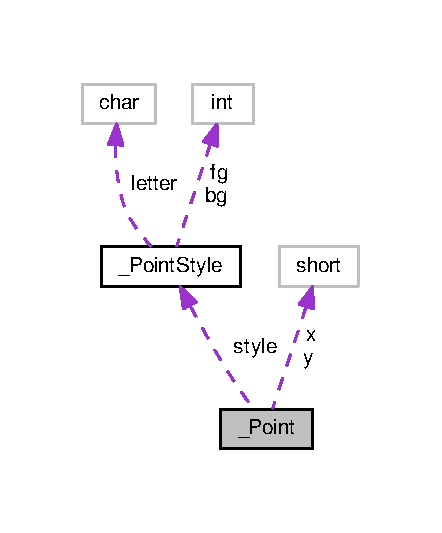
\includegraphics[width=213pt]{struct___point__coll__graph}
\end{center}
\end{figure}
\subsection*{Public Member Functions}
\begin{DoxyCompactItemize}
\item 
\mbox{\hyperlink{struct___point}{\+\_\+\+Point}} \& \mbox{\hyperlink{struct___point_acf5181d8cc6c6bd73a73aa1da2d980cb}{operator=}} (\mbox{\hyperlink{struct___point}{\+\_\+\+Point}} p)
\end{DoxyCompactItemize}
\subsection*{Public Attributes}
\begin{DoxyCompactItemize}
\item 
short \mbox{\hyperlink{struct___point_a1c1cb9f2bfc0c90f1079661912b69e48}{x}}
\item 
short \mbox{\hyperlink{struct___point_af63bdd5a8c2fcf3fc4701a1cc6a421df}{y}}
\item 
\mbox{\hyperlink{common_8h_afd9cb36d6ef309c77ea1e3177e19c623}{Point\+Style}} \mbox{\hyperlink{struct___point_af909fc976d09ac1f11878b4bdcfa10ca}{style}}
\end{DoxyCompactItemize}


\subsection{Detailed Description}
Coordinates of the cell in console window 
\begin{DoxyParams}{Parameters}
{\em \{short\}} & x -\/ x coordinate in console window \\
\hline
{\em \{short\}} & y -\/ y coordinate in console window \\
\hline
\end{DoxyParams}


Definition at line 38 of file common.\+h.



\subsection{Member Function Documentation}
\mbox{\Hypertarget{struct___point_acf5181d8cc6c6bd73a73aa1da2d980cb}\label{struct___point_acf5181d8cc6c6bd73a73aa1da2d980cb}} 
\index{\_Point@{\_Point}!operator=@{operator=}}
\index{operator=@{operator=}!\_Point@{\_Point}}
\subsubsection{\texorpdfstring{operator=()}{operator=()}}
{\footnotesize\ttfamily \mbox{\hyperlink{common_8h_aa9cfdb80b4ca12013a2de8a3b9b97981}{Point}} \& Point\+::operator= (\begin{DoxyParamCaption}\item[{\mbox{\hyperlink{struct___point}{\+\_\+\+Point}}}]{p }\end{DoxyParamCaption})}

Operation \char`\"{}=\char`\"{} override for the Point type 
\begin{DoxyParams}{Parameters}
{\em \{\+Point\}} & p -\/ the obgect, parameters of which are being copied \\
\hline
\end{DoxyParams}
\begin{DoxyReturn}{Returns}
\{Point\&\} a pointer to an object @override 
\end{DoxyReturn}


Definition at line 23 of file common.\+cpp.



\subsection{Member Data Documentation}
\mbox{\Hypertarget{struct___point_af909fc976d09ac1f11878b4bdcfa10ca}\label{struct___point_af909fc976d09ac1f11878b4bdcfa10ca}} 
\index{\_Point@{\_Point}!style@{style}}
\index{style@{style}!\_Point@{\_Point}}
\subsubsection{\texorpdfstring{style}{style}}
{\footnotesize\ttfamily \mbox{\hyperlink{common_8h_afd9cb36d6ef309c77ea1e3177e19c623}{Point\+Style}} \+\_\+\+Point\+::style}



Definition at line 41 of file common.\+h.

\mbox{\Hypertarget{struct___point_a1c1cb9f2bfc0c90f1079661912b69e48}\label{struct___point_a1c1cb9f2bfc0c90f1079661912b69e48}} 
\index{\_Point@{\_Point}!x@{x}}
\index{x@{x}!\_Point@{\_Point}}
\subsubsection{\texorpdfstring{x}{x}}
{\footnotesize\ttfamily short \+\_\+\+Point\+::x}



Definition at line 40 of file common.\+h.

\mbox{\Hypertarget{struct___point_af63bdd5a8c2fcf3fc4701a1cc6a421df}\label{struct___point_af63bdd5a8c2fcf3fc4701a1cc6a421df}} 
\index{\_Point@{\_Point}!y@{y}}
\index{y@{y}!\_Point@{\_Point}}
\subsubsection{\texorpdfstring{y}{y}}
{\footnotesize\ttfamily short \+\_\+\+Point\+::y}



Definition at line 40 of file common.\+h.



The documentation for this struct was generated from the following files\+:\begin{DoxyCompactItemize}
\item 
Libraries/\+Common/\mbox{\hyperlink{common_8h}{common.\+h}}\item 
Libraries/\+Common/\mbox{\hyperlink{common_8cpp}{common.\+cpp}}\end{DoxyCompactItemize}

\hypertarget{struct___point_style}{\section{\-\_\-\-Point\-Style Struct Reference}
\label{struct___point_style}\index{\-\_\-\-Point\-Style@{\-\_\-\-Point\-Style}}
}


{\ttfamily \#include $<$common.\-h$>$}



Collaboration diagram for \-\_\-\-Point\-Style\-:
\nopagebreak
\begin{figure}[H]
\begin{center}
\leavevmode
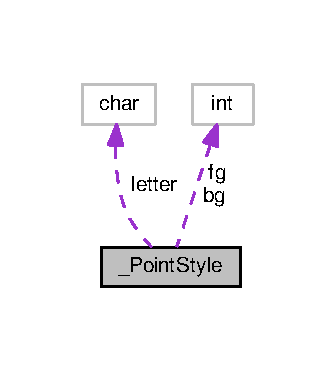
\includegraphics[width=161pt]{struct___point_style__coll__graph}
\end{center}
\end{figure}
\subsection*{Public Member Functions}
\begin{DoxyCompactItemize}
\item 
\hyperlink{struct___point_style}{\-\_\-\-Point\-Style} \& \hyperlink{struct___point_style_a1928e8b7e2cf5588abbccf6774bd1714}{operator=} (\hyperlink{struct___point_style}{\-\_\-\-Point\-Style} ps)
\end{DoxyCompactItemize}
\subsection*{Public Attributes}
\begin{DoxyCompactItemize}
\item 
char \hyperlink{struct___point_style_aa4cf23b21f61b08b05ff90b37fb26bc8}{letter}
\item 
int \hyperlink{struct___point_style_aad357bccd6e6759fc8575d3354d2bc7b}{fg}
\item 
int \hyperlink{struct___point_style_a0f1cb3b870284fd00ca8bdc2cbb782ca}{bg}
\end{DoxyCompactItemize}


\subsection{Detailed Description}
Style of the cell in console window 
\begin{DoxyParams}{Parameters}
{\em \{char\}} & letter -\/ symbol in the cell \\
\hline
{\em \{short\}} & fg -\/ foreground color of the cell \\
\hline
{\em \{short\}} & bg -\/ beckground color of the cell \\
\hline
\end{DoxyParams}


Definition at line 26 of file common.\-h.



\subsection{Member Function Documentation}
\hypertarget{struct___point_style_a1928e8b7e2cf5588abbccf6774bd1714}{\index{\-\_\-\-Point\-Style@{\-\_\-\-Point\-Style}!operator=@{operator=}}
\index{operator=@{operator=}!_PointStyle@{\-\_\-\-Point\-Style}}
\subsubsection[{operator=}]{\setlength{\rightskip}{0pt plus 5cm}{\bf Point\-Style} \& Point\-Style\-::operator= (
\begin{DoxyParamCaption}
\item[{{\bf \-\_\-\-Point\-Style}}]{ps}
\end{DoxyParamCaption}
)}}\label{struct___point_style_a1928e8b7e2cf5588abbccf6774bd1714}
Operation \char`\"{}=\char`\"{} override for the Point\-Style type 
\begin{DoxyParams}{Parameters}
{\em \{\-Point\-Style\}} & ps -\/ the obgect, parameters of which are being copied \\
\hline
\end{DoxyParams}
\begin{DoxyReturn}{Returns}
\{Point\-Style\&\} a pointer to an object  
\end{DoxyReturn}


Definition at line 9 of file common.\-cpp.



\subsection{Member Data Documentation}
\hypertarget{struct___point_style_a0f1cb3b870284fd00ca8bdc2cbb782ca}{\index{\-\_\-\-Point\-Style@{\-\_\-\-Point\-Style}!bg@{bg}}
\index{bg@{bg}!_PointStyle@{\-\_\-\-Point\-Style}}
\subsubsection[{bg}]{\setlength{\rightskip}{0pt plus 5cm}int \-\_\-\-Point\-Style\-::bg}}\label{struct___point_style_a0f1cb3b870284fd00ca8bdc2cbb782ca}


Definition at line 29 of file common.\-h.

\hypertarget{struct___point_style_aad357bccd6e6759fc8575d3354d2bc7b}{\index{\-\_\-\-Point\-Style@{\-\_\-\-Point\-Style}!fg@{fg}}
\index{fg@{fg}!_PointStyle@{\-\_\-\-Point\-Style}}
\subsubsection[{fg}]{\setlength{\rightskip}{0pt plus 5cm}int \-\_\-\-Point\-Style\-::fg}}\label{struct___point_style_aad357bccd6e6759fc8575d3354d2bc7b}


Definition at line 29 of file common.\-h.

\hypertarget{struct___point_style_aa4cf23b21f61b08b05ff90b37fb26bc8}{\index{\-\_\-\-Point\-Style@{\-\_\-\-Point\-Style}!letter@{letter}}
\index{letter@{letter}!_PointStyle@{\-\_\-\-Point\-Style}}
\subsubsection[{letter}]{\setlength{\rightskip}{0pt plus 5cm}char \-\_\-\-Point\-Style\-::letter}}\label{struct___point_style_aa4cf23b21f61b08b05ff90b37fb26bc8}


Definition at line 28 of file common.\-h.



The documentation for this struct was generated from the following files\-:\begin{DoxyCompactItemize}
\item 
/home/travis/build/echo-\/team/\-Snoke/\-Libraries/\-Common/\hyperlink{common_8h}{common.\-h}\item 
/home/travis/build/echo-\/team/\-Snoke/\-Libraries/\-Common/\hyperlink{common_8cpp}{common.\-cpp}\end{DoxyCompactItemize}

\hypertarget{class_ball}{\section{Ball Class Reference}
\label{class_ball}\index{Ball@{Ball}}
}


{\ttfamily \#include $<$ball.\-h$>$}



Collaboration diagram for Ball\-:
\nopagebreak
\begin{figure}[H]
\begin{center}
\leavevmode
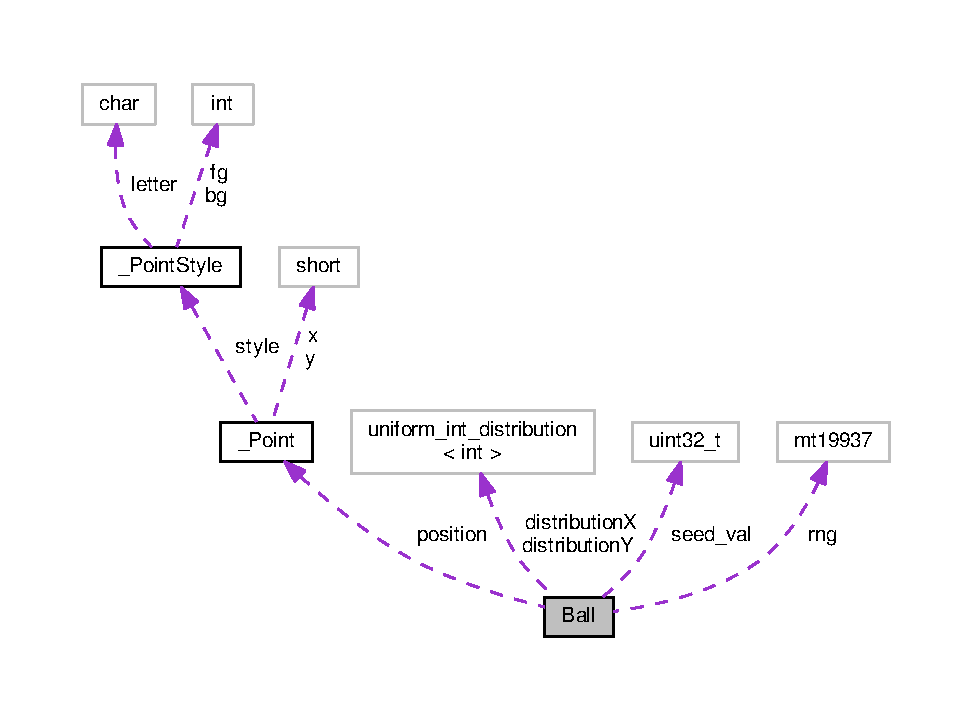
\includegraphics[width=350pt]{class_ball__coll__graph}
\end{center}
\end{figure}
\subsection*{Public Member Functions}
\begin{DoxyCompactItemize}
\item 
bool \hyperlink{class_ball_a1907f13fdfb320a19180efec2a56e39c}{init} (\hyperlink{common_8h_aa9cfdb80b4ca12013a2de8a3b9b97981}{Point} dim)
\item 
bool \hyperlink{class_ball_a60fd40459426366242d18d85b3b50c2c}{generate\-Ball} (\hyperlink{class_labyrinth}{Labyrinth} labyrinth, \hyperlink{common_8h_aa9cfdb80b4ca12013a2de8a3b9b97981}{Point} $\ast$change\mbox{[}2\mbox{]}, int change\-Size)
\item 
\hyperlink{common_8h_aa9cfdb80b4ca12013a2de8a3b9b97981}{Point} \hyperlink{class_ball_a14b9a607402be58e7a0a0ab053df5f82}{get\-Coords} ()
\end{DoxyCompactItemize}
\subsection*{Private Attributes}
\begin{DoxyCompactItemize}
\item 
\hyperlink{common_8h_aa9cfdb80b4ca12013a2de8a3b9b97981}{Point} \hyperlink{class_ball_abd10a53eda37a2c541ad5dfbbea27f81}{position}
\item 
std\-::mt19937 \hyperlink{class_ball_ae3c68e21e0801b657b980380ab6a4bb2}{rng}
\item 
uint32\-\_\-t \hyperlink{class_ball_ad6e67b032167a7d9db9630bc5ab2e613}{seed\-\_\-val}
\item 
std\-::uniform\-\_\-int\-\_\-distribution\\*
$<$ int $>$ \hyperlink{class_ball_a558a48196bdb4ea389519ab7c0138216}{distribution\-X}
\item 
std\-::uniform\-\_\-int\-\_\-distribution\\*
$<$ int $>$ \hyperlink{class_ball_a9a8e67dcc49382448848c497ff7ede25}{distribution\-Y}
\end{DoxyCompactItemize}


\subsection{Detailed Description}
Describes the \hyperlink{class_ball}{Ball} entity of the game 
\begin{DoxyParams}{Parameters}
{\em \{\-Point\}} & position -\/ a Coordinates(x, y) of a \hyperlink{class_ball}{Ball} in the Console window \\
\hline
{\em \{mt19937\}} & rng -\/ the variable, responible for the 'random' during the game \\
\hline
{\em \{uint32\-\_\-t\}} & seed\-\_\-val -\/ value 'feeded' to the 'random' generator \\
\hline
{\em \{uniform\-\_\-int\-\_\-distribution$<$int$>$\}} & distribution\-X -\/ an equally likely int distribution for x coordinate of a \hyperlink{class_ball}{Ball} \\
\hline
{\em \{uniform\-\_\-int\-\_\-distribution$<$int$>$\}} & distribution\-Y -\/ an equally likely int distribution for y coordinate of a \hyperlink{class_ball}{Ball} \\
\hline
\end{DoxyParams}


Definition at line 17 of file ball.\-h.



\subsection{Member Function Documentation}
\hypertarget{class_ball_a60fd40459426366242d18d85b3b50c2c}{\index{Ball@{Ball}!generate\-Ball@{generate\-Ball}}
\index{generate\-Ball@{generate\-Ball}!Ball@{Ball}}
\subsubsection[{generate\-Ball}]{\setlength{\rightskip}{0pt plus 5cm}bool Ball\-::generate\-Ball (
\begin{DoxyParamCaption}
\item[{{\bf Labyrinth}}]{labyrinth, }
\item[{{\bf Point} $\ast$}]{change\mbox{[}2\mbox{]}, }
\item[{int}]{change\-Size}
\end{DoxyParamCaption}
)}}\label{class_ball_a60fd40459426366242d18d85b3b50c2c}
Generate the \hyperlink{class_ball}{Ball} 
\begin{DoxyParams}{Parameters}
{\em \{\-Labyrinth\}} & labyrinth -\/ the current state of the labyrinth object for intersection checking \\
\hline
\end{DoxyParams}
\begin{DoxyReturn}{Returns}
\{bool\} -\/ mark of whether the ball was successfully generated 
\end{DoxyReturn}
Generate numbers until u get a free spot

Definition at line 23 of file ball.\-cpp.



Here is the call graph for this function\-:
\nopagebreak
\begin{figure}[H]
\begin{center}
\leavevmode
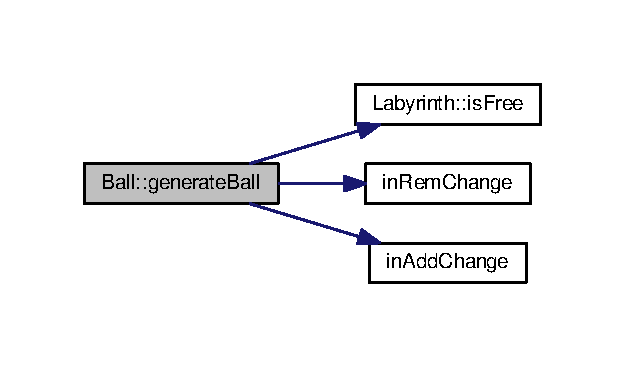
\includegraphics[width=300pt]{class_ball_a60fd40459426366242d18d85b3b50c2c_cgraph}
\end{center}
\end{figure}




Here is the caller graph for this function\-:
\nopagebreak
\begin{figure}[H]
\begin{center}
\leavevmode
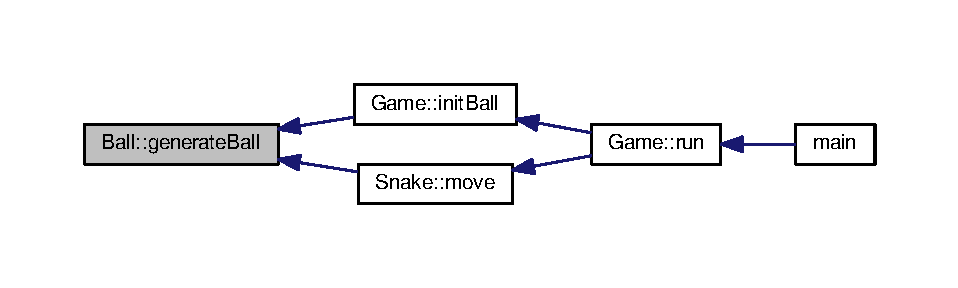
\includegraphics[width=350pt]{class_ball_a60fd40459426366242d18d85b3b50c2c_icgraph}
\end{center}
\end{figure}


\hypertarget{class_ball_a14b9a607402be58e7a0a0ab053df5f82}{\index{Ball@{Ball}!get\-Coords@{get\-Coords}}
\index{get\-Coords@{get\-Coords}!Ball@{Ball}}
\subsubsection[{get\-Coords}]{\setlength{\rightskip}{0pt plus 5cm}{\bf Point} Ball\-::get\-Coords (
\begin{DoxyParamCaption}
{}
\end{DoxyParamCaption}
)}}\label{class_ball_a14b9a607402be58e7a0a0ab053df5f82}
Get the ball coords without giving the direct access \begin{DoxyReturn}{Returns}
\{Point\} 
\end{DoxyReturn}


Definition at line 47 of file ball.\-cpp.



Here is the caller graph for this function\-:
\nopagebreak
\begin{figure}[H]
\begin{center}
\leavevmode
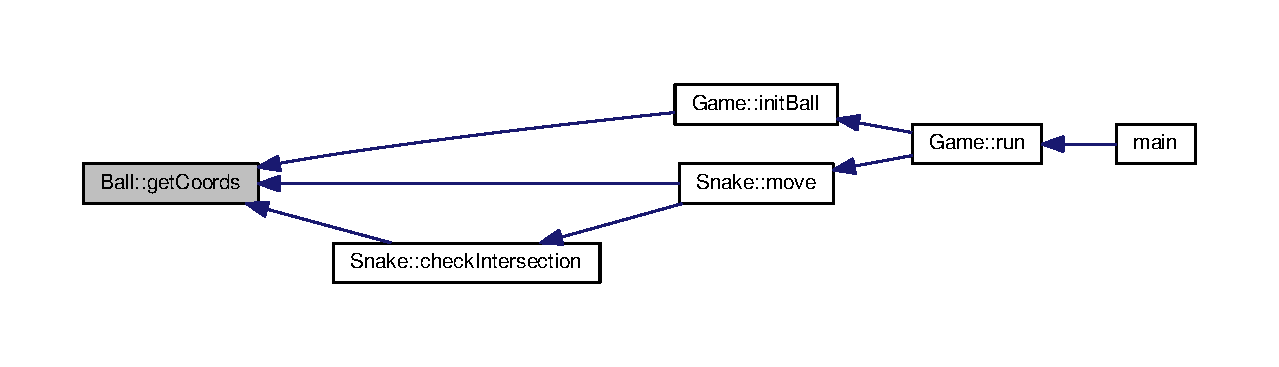
\includegraphics[width=350pt]{class_ball_a14b9a607402be58e7a0a0ab053df5f82_icgraph}
\end{center}
\end{figure}


\hypertarget{class_ball_a1907f13fdfb320a19180efec2a56e39c}{\index{Ball@{Ball}!init@{init}}
\index{init@{init}!Ball@{Ball}}
\subsubsection[{init}]{\setlength{\rightskip}{0pt plus 5cm}bool Ball\-::init (
\begin{DoxyParamCaption}
\item[{{\bf Point}}]{field\-Size}
\end{DoxyParamCaption}
)}}\label{class_ball_a1907f13fdfb320a19180efec2a56e39c}
Initialization 
\begin{DoxyParams}{Parameters}
{\em \{\-Point\}} & field\-Size -\/ the size of the game field(x, y) \\
\hline
\end{DoxyParams}
\begin{DoxyReturn}{Returns}
\{bool\} -\/ mark of successful initialization 
\end{DoxyReturn}


Definition at line 8 of file ball.\-cpp.



Here is the caller graph for this function\-:
\nopagebreak
\begin{figure}[H]
\begin{center}
\leavevmode
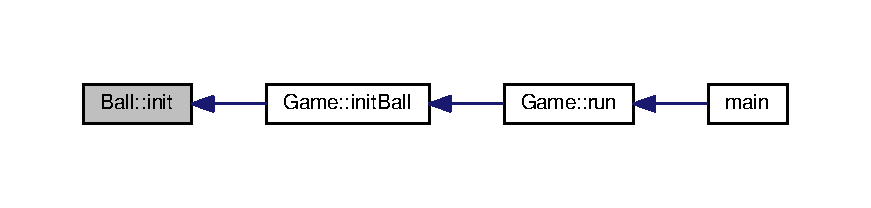
\includegraphics[width=350pt]{class_ball_a1907f13fdfb320a19180efec2a56e39c_icgraph}
\end{center}
\end{figure}




\subsection{Member Data Documentation}
\hypertarget{class_ball_a558a48196bdb4ea389519ab7c0138216}{\index{Ball@{Ball}!distribution\-X@{distribution\-X}}
\index{distribution\-X@{distribution\-X}!Ball@{Ball}}
\subsubsection[{distribution\-X}]{\setlength{\rightskip}{0pt plus 5cm}std\-::uniform\-\_\-int\-\_\-distribution$<$int$>$ Ball\-::distribution\-X\hspace{0.3cm}{\ttfamily [private]}}}\label{class_ball_a558a48196bdb4ea389519ab7c0138216}


Definition at line 23 of file ball.\-h.

\hypertarget{class_ball_a9a8e67dcc49382448848c497ff7ede25}{\index{Ball@{Ball}!distribution\-Y@{distribution\-Y}}
\index{distribution\-Y@{distribution\-Y}!Ball@{Ball}}
\subsubsection[{distribution\-Y}]{\setlength{\rightskip}{0pt plus 5cm}std\-::uniform\-\_\-int\-\_\-distribution$<$int$>$ Ball\-::distribution\-Y\hspace{0.3cm}{\ttfamily [private]}}}\label{class_ball_a9a8e67dcc49382448848c497ff7ede25}


Definition at line 24 of file ball.\-h.

\hypertarget{class_ball_abd10a53eda37a2c541ad5dfbbea27f81}{\index{Ball@{Ball}!position@{position}}
\index{position@{position}!Ball@{Ball}}
\subsubsection[{position}]{\setlength{\rightskip}{0pt plus 5cm}{\bf Point} Ball\-::position\hspace{0.3cm}{\ttfamily [private]}}}\label{class_ball_abd10a53eda37a2c541ad5dfbbea27f81}


Definition at line 20 of file ball.\-h.

\hypertarget{class_ball_ae3c68e21e0801b657b980380ab6a4bb2}{\index{Ball@{Ball}!rng@{rng}}
\index{rng@{rng}!Ball@{Ball}}
\subsubsection[{rng}]{\setlength{\rightskip}{0pt plus 5cm}std\-::mt19937 Ball\-::rng\hspace{0.3cm}{\ttfamily [private]}}}\label{class_ball_ae3c68e21e0801b657b980380ab6a4bb2}


Definition at line 21 of file ball.\-h.

\hypertarget{class_ball_ad6e67b032167a7d9db9630bc5ab2e613}{\index{Ball@{Ball}!seed\-\_\-val@{seed\-\_\-val}}
\index{seed\-\_\-val@{seed\-\_\-val}!Ball@{Ball}}
\subsubsection[{seed\-\_\-val}]{\setlength{\rightskip}{0pt plus 5cm}uint32\-\_\-t Ball\-::seed\-\_\-val\hspace{0.3cm}{\ttfamily [private]}}}\label{class_ball_ad6e67b032167a7d9db9630bc5ab2e613}


Definition at line 22 of file ball.\-h.



The documentation for this class was generated from the following files\-:\begin{DoxyCompactItemize}
\item 
/home/travis/build/echo-\/team/\-Snoke/\-Libraries/\-Ball/\hyperlink{ball_8h}{ball.\-h}\item 
/home/travis/build/echo-\/team/\-Snoke/\-Libraries/\-Ball/\hyperlink{ball_8cpp}{ball.\-cpp}\end{DoxyCompactItemize}

\hypertarget{class_game}{\section{Game Class Reference}
\label{class_game}\index{Game@{Game}}
}


{\ttfamily \#include $<$game.\-h$>$}



Collaboration diagram for Game\-:
\nopagebreak
\begin{figure}[H]
\begin{center}
\leavevmode
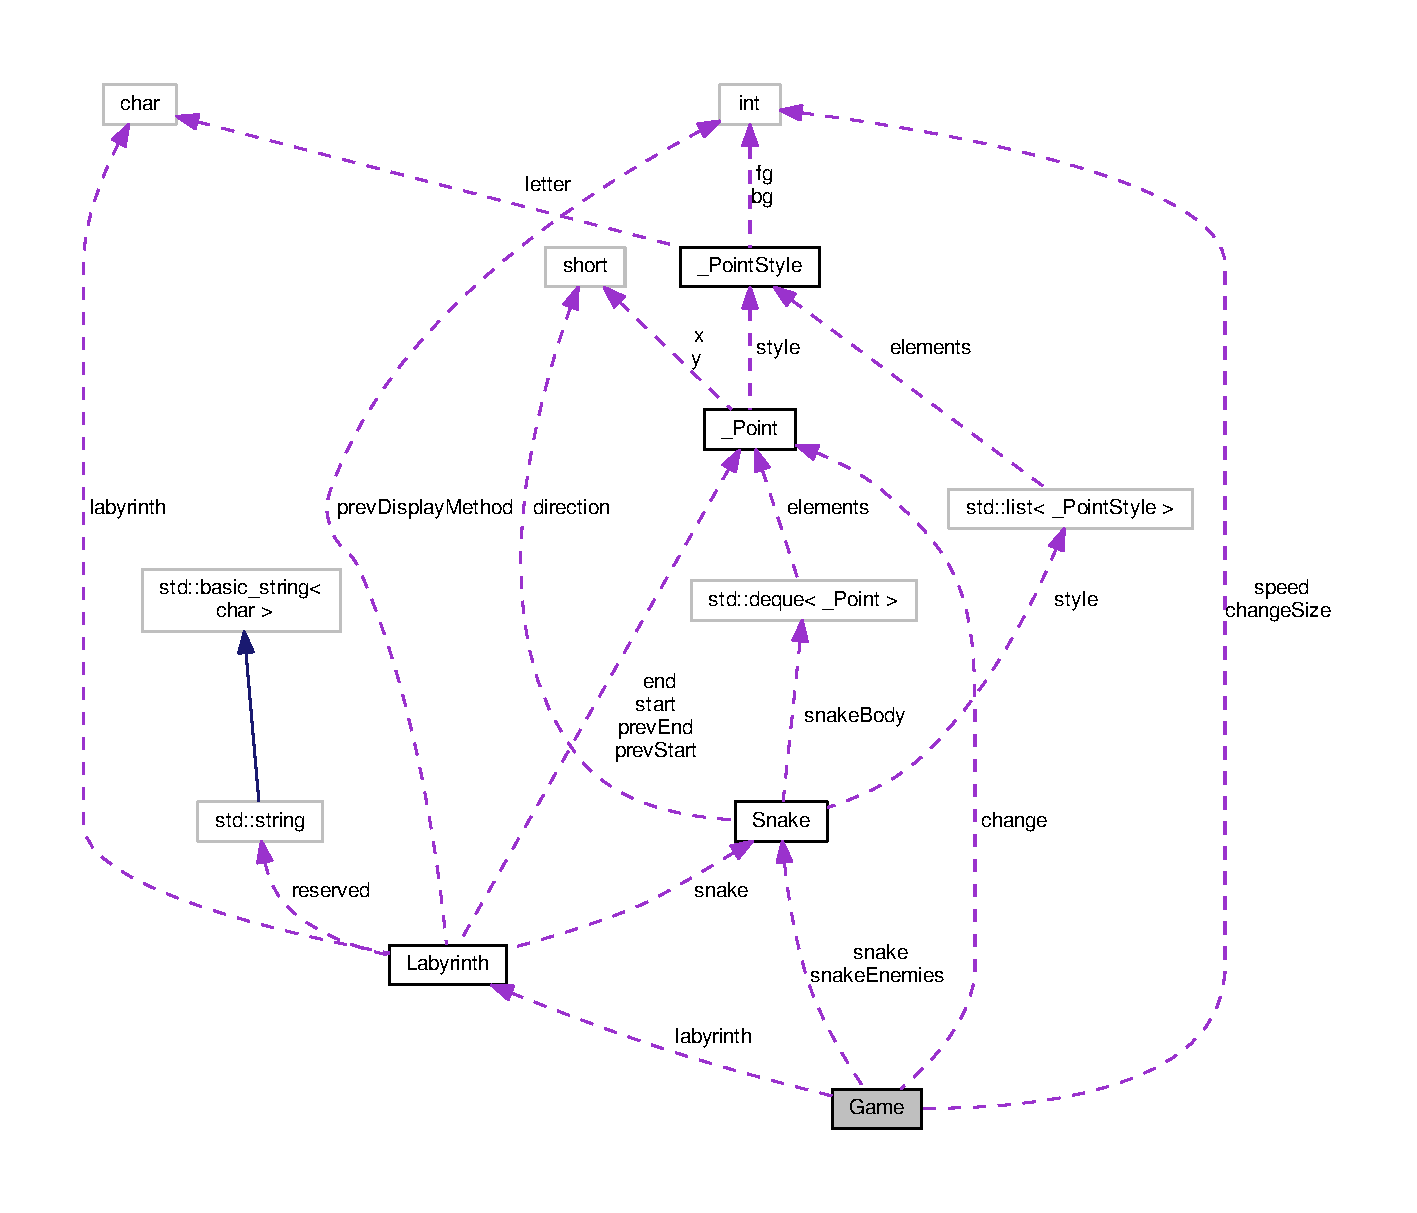
\includegraphics[width=350pt]{class_game__coll__graph}
\end{center}
\end{figure}
\subsection*{Public Member Functions}
\begin{DoxyCompactItemize}
\item 
bool \hyperlink{class_game_a66e1800ff072c0b4e737ac51430630db}{init} (int size=20, int sp=100)
\item 
int \hyperlink{class_game_a99fb161fbbe87d25a8b73265a0611e58}{run} ()
\end{DoxyCompactItemize}
\subsection*{Private Member Functions}
\begin{DoxyCompactItemize}
\item 
void \hyperlink{class_game_a5f3fdd22fa8ae39d6912ee3ff029ea46}{set\-Speed} (int sp)
\item 
bool \hyperlink{class_game_a0e8435182e77e921b5ba0471a8bfb20d}{init\-Snake} (\hyperlink{common_8h_aa9cfdb80b4ca12013a2de8a3b9b97981}{Point} begin, int dir, int length)
\item 
bool \hyperlink{class_game_a3702238c3fef205d19d1cb4bbc471c5c}{init\-Ball} (\hyperlink{class_ball}{Ball} $\ast$ball)
\item 
bool \hyperlink{class_game_aa73688f1ba069a3f1989884099c58449}{wipe\-Change} (\hyperlink{common_8h_aa9cfdb80b4ca12013a2de8a3b9b97981}{Point} $\ast$$\ast$\hyperlink{class_game_a87f9c54e60a724de2644769cd917dbce}{change}, int size)
\end{DoxyCompactItemize}
\subsection*{Private Attributes}
\begin{DoxyCompactItemize}
\item 
int \hyperlink{class_game_a02a58acc040d6d014e02832453695ef5}{speed}
\item 
int \hyperlink{class_game_ae959d08e508fcef98dd07a2b9cd82e65}{change\-Size}
\item 
\hyperlink{class_snake}{Snake} \hyperlink{class_game_ab77bfcc312425811000819791ea7668e}{snake}
\item 
\hyperlink{class_snake}{Snake} $\ast$ \hyperlink{class_game_ab7d2baa4a2dbcb64fc1611aac709fe40}{snake\-Enemies}
\item 
\hyperlink{class_labyrinth}{Labyrinth} \hyperlink{class_game_a92148f2659c019b331e9da7deadbd8bc}{labyrinth}
\item 
\hyperlink{common_8h_aa9cfdb80b4ca12013a2de8a3b9b97981}{Point} $\ast$ \hyperlink{class_game_a87f9c54e60a724de2644769cd917dbce}{change} \mbox{[}2\mbox{]}
\end{DoxyCompactItemize}


\subsection{Detailed Description}
Main game class 
\begin{DoxyParams}{Parameters}
{\em \{int\}} & speed -\/ game refresh spee(in milliseconds) \\
\hline
{\em \{int\}} & change\-Size -\/ the size of the change sub-\/arrays \\
\hline
{\em \{\-Snake\}} & snake -\/ the local\-\_\-player-\/controlled snake entity \\
\hline
{\em \{\-Snake$\ast$\}} & snake\-Enemies -\/ the remotely controlled snake entities \\
\hline
{\em \{\-Labyrinth\}} & labyrinth -\/ object containing labyrinth, displaying it, etc \\
\hline
{\em \{\-Point$\ast$\}} & change -\/ 2-\/dim array containing changes for the labyrinth \\
\hline
\end{DoxyParams}


Definition at line 19 of file game.\-h.



\subsection{Member Function Documentation}
\hypertarget{class_game_a66e1800ff072c0b4e737ac51430630db}{\index{Game@{Game}!init@{init}}
\index{init@{init}!Game@{Game}}
\subsubsection[{init}]{\setlength{\rightskip}{0pt plus 5cm}bool Game\-::init (
\begin{DoxyParamCaption}
\item[{int}]{size = {\ttfamily 20}, }
\item[{int}]{speed = {\ttfamily 100}}
\end{DoxyParamCaption}
)}}\label{class_game_a66e1800ff072c0b4e737ac51430630db}
Initializes game 
\begin{DoxyParams}{Parameters}
{\em \{int\}} & size -\/ size of the game field(size -\/ 2 columns, size/2 -\/ 2 rows) \\
\hline
{\em \{int\}} & speed -\/ speed of the game(1 / refresh rate) in milliseconds \\
\hline
\end{DoxyParams}
\begin{DoxyReturn}{Returns}
\{bool\} -\/ mark of successful initialization 
\end{DoxyReturn}
Initializing the change array, containing Points to be changed in the labyrinth

Definition at line 16 of file game.\-cpp.



Here is the call graph for this function\-:
\nopagebreak
\begin{figure}[H]
\begin{center}
\leavevmode
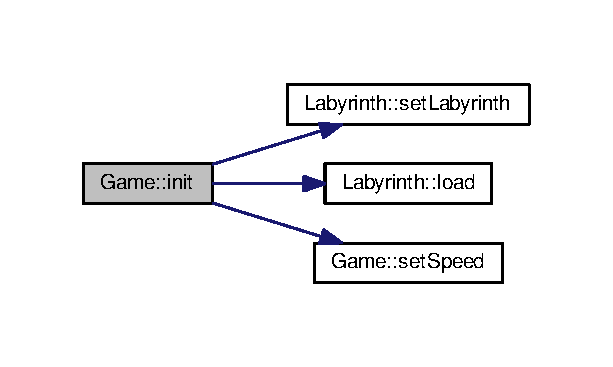
\includegraphics[width=294pt]{class_game_a66e1800ff072c0b4e737ac51430630db_cgraph}
\end{center}
\end{figure}




Here is the caller graph for this function\-:
\nopagebreak
\begin{figure}[H]
\begin{center}
\leavevmode
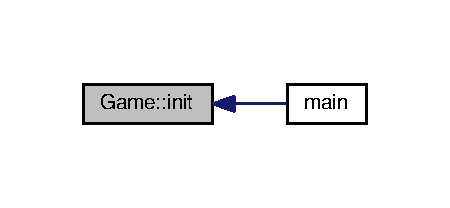
\includegraphics[width=216pt]{class_game_a66e1800ff072c0b4e737ac51430630db_icgraph}
\end{center}
\end{figure}


\hypertarget{class_game_a3702238c3fef205d19d1cb4bbc471c5c}{\index{Game@{Game}!init\-Ball@{init\-Ball}}
\index{init\-Ball@{init\-Ball}!Game@{Game}}
\subsubsection[{init\-Ball}]{\setlength{\rightskip}{0pt plus 5cm}bool Game\-::init\-Ball (
\begin{DoxyParamCaption}
\item[{{\bf Ball} $\ast$}]{ball}
\end{DoxyParamCaption}
)\hspace{0.3cm}{\ttfamily [private]}}}\label{class_game_a3702238c3fef205d19d1cb4bbc471c5c}
\hyperlink{class_ball}{Ball} initialization with labyrinth updating 
\begin{DoxyParams}{Parameters}
{\em \{\-Ball$\ast$\}} & ball -\/ a pointer to a \hyperlink{class_ball}{Ball}, which is being initialized \\
\hline
\end{DoxyParams}
\begin{DoxyReturn}{Returns}
\{bool\} -\/ mark of succesful initialization 
\end{DoxyReturn}


Definition at line 155 of file game.\-cpp.



Here is the call graph for this function\-:
\nopagebreak
\begin{figure}[H]
\begin{center}
\leavevmode
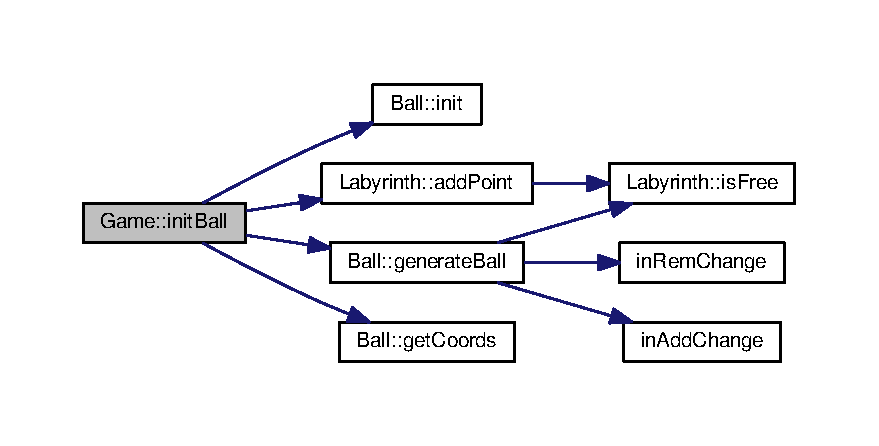
\includegraphics[width=350pt]{class_game_a3702238c3fef205d19d1cb4bbc471c5c_cgraph}
\end{center}
\end{figure}




Here is the caller graph for this function\-:
\nopagebreak
\begin{figure}[H]
\begin{center}
\leavevmode
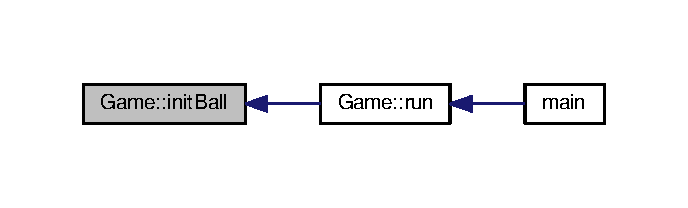
\includegraphics[width=330pt]{class_game_a3702238c3fef205d19d1cb4bbc471c5c_icgraph}
\end{center}
\end{figure}


\hypertarget{class_game_a0e8435182e77e921b5ba0471a8bfb20d}{\index{Game@{Game}!init\-Snake@{init\-Snake}}
\index{init\-Snake@{init\-Snake}!Game@{Game}}
\subsubsection[{init\-Snake}]{\setlength{\rightskip}{0pt plus 5cm}bool Game\-::init\-Snake (
\begin{DoxyParamCaption}
\item[{{\bf Point}}]{begin, }
\item[{int}]{dir, }
\item[{int}]{length}
\end{DoxyParamCaption}
)\hspace{0.3cm}{\ttfamily [private]}}}\label{class_game_a0e8435182e77e921b5ba0471a8bfb20d}
\hyperlink{class_snake}{Snake} initialization with labyrinth updating 
\begin{DoxyParams}{Parameters}
{\em \{\-Point\}} & begin -\/ starting Point of a snake(where the tail segment will be situated) \\
\hline
{\em \{short\}} & dir -\/ direction of snake's 'growth' as well as it's starting direction \\
\hline
{\em \{int\}} & length -\/ the length of a 'new born' snake \\
\hline
\end{DoxyParams}
\begin{DoxyReturn}{Returns}
\{bool\} -\/ mark of whether the snake is successfully initialized 
\end{DoxyReturn}


Definition at line 141 of file game.\-cpp.



Here is the call graph for this function\-:
\nopagebreak
\begin{figure}[H]
\begin{center}
\leavevmode
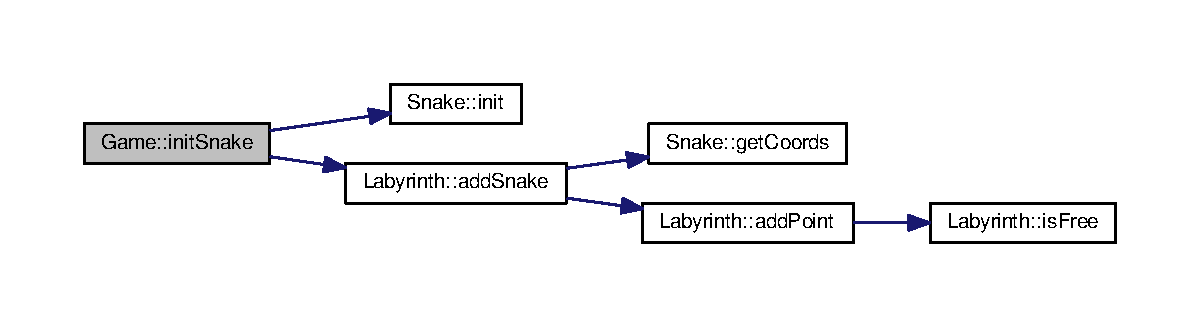
\includegraphics[width=350pt]{class_game_a0e8435182e77e921b5ba0471a8bfb20d_cgraph}
\end{center}
\end{figure}




Here is the caller graph for this function\-:
\nopagebreak
\begin{figure}[H]
\begin{center}
\leavevmode
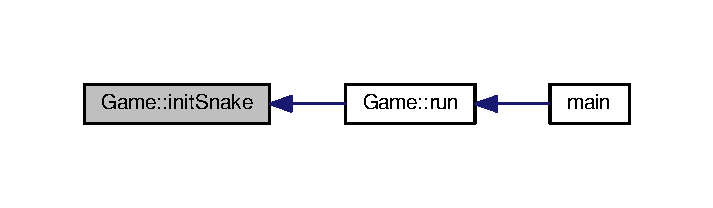
\includegraphics[width=342pt]{class_game_a0e8435182e77e921b5ba0471a8bfb20d_icgraph}
\end{center}
\end{figure}


\hypertarget{class_game_a99fb161fbbe87d25a8b73265a0611e58}{\index{Game@{Game}!run@{run}}
\index{run@{run}!Game@{Game}}
\subsubsection[{run}]{\setlength{\rightskip}{0pt plus 5cm}int Game\-::run (
\begin{DoxyParamCaption}
{}
\end{DoxyParamCaption}
)}}\label{class_game_a99fb161fbbe87d25a8b73265a0611e58}
Main game loop \begin{DoxyReturn}{Returns}
\{int\} -\/ the exit code 
\end{DoxyReturn}
Block initializing ncurses console in the current console window, and setting some parameters

Initializing snake by giving it the starting position, direction of growth and starting length

Initializing the \hyperlink{class_ball}{Ball} and generating it on the field

displaying the starting state of labyrinth

Setting the flag for the next iteration check Moving the snake and getting the Points of a labyrinth which are to be changed in change array

Updating labyrinth with change array Points and displaying/deleting added/removed Points

Definition at line 38 of file game.\-cpp.



Here is the call graph for this function\-:
\nopagebreak
\begin{figure}[H]
\begin{center}
\leavevmode
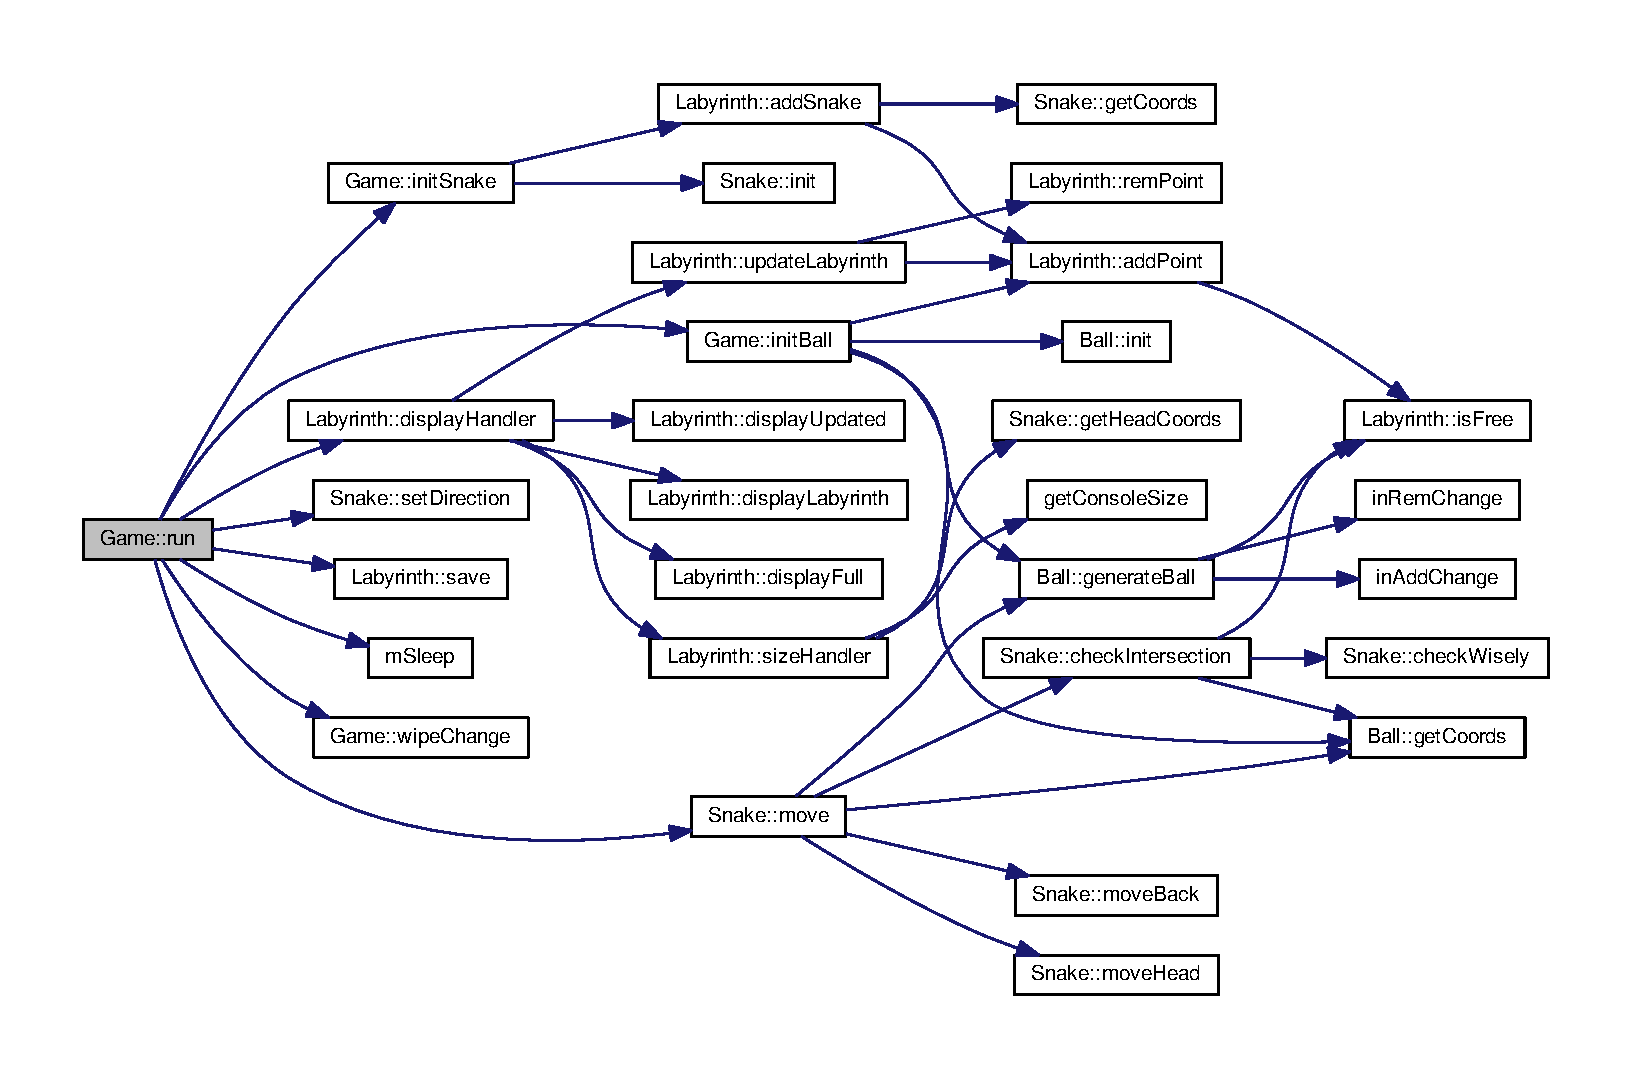
\includegraphics[width=350pt]{class_game_a99fb161fbbe87d25a8b73265a0611e58_cgraph}
\end{center}
\end{figure}




Here is the caller graph for this function\-:
\nopagebreak
\begin{figure}[H]
\begin{center}
\leavevmode
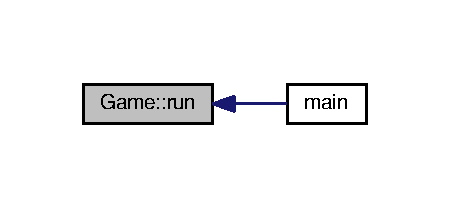
\includegraphics[width=216pt]{class_game_a99fb161fbbe87d25a8b73265a0611e58_icgraph}
\end{center}
\end{figure}


\hypertarget{class_game_a5f3fdd22fa8ae39d6912ee3ff029ea46}{\index{Game@{Game}!set\-Speed@{set\-Speed}}
\index{set\-Speed@{set\-Speed}!Game@{Game}}
\subsubsection[{set\-Speed}]{\setlength{\rightskip}{0pt plus 5cm}void Game\-::set\-Speed (
\begin{DoxyParamCaption}
\item[{int}]{speed}
\end{DoxyParamCaption}
)\hspace{0.3cm}{\ttfamily [private]}}}\label{class_game_a5f3fdd22fa8ae39d6912ee3ff029ea46}
The method to change the game speed without giving the direct access and some error handling 
\begin{DoxyParams}{Parameters}
{\em \{int\}} & speed -\/ speed of the game(1 / refresh rate) in milliseconds \\
\hline
\end{DoxyParams}


Definition at line 192 of file game.\-cpp.



Here is the caller graph for this function\-:
\nopagebreak
\begin{figure}[H]
\begin{center}
\leavevmode
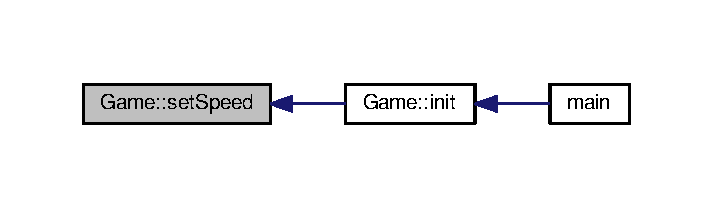
\includegraphics[width=342pt]{class_game_a5f3fdd22fa8ae39d6912ee3ff029ea46_icgraph}
\end{center}
\end{figure}


\hypertarget{class_game_aa73688f1ba069a3f1989884099c58449}{\index{Game@{Game}!wipe\-Change@{wipe\-Change}}
\index{wipe\-Change@{wipe\-Change}!Game@{Game}}
\subsubsection[{wipe\-Change}]{\setlength{\rightskip}{0pt plus 5cm}bool Game\-::wipe\-Change (
\begin{DoxyParamCaption}
\item[{{\bf Point} $\ast$$\ast$}]{change, }
\item[{int}]{size}
\end{DoxyParamCaption}
)\hspace{0.3cm}{\ttfamily [private]}}}\label{class_game_aa73688f1ba069a3f1989884099c58449}
Initialization of the change array 
\begin{DoxyParams}{Parameters}
{\em \{\-Point$\ast$$\ast$\}} & change -\/ The pointer to an array \\
\hline
{\em \{int\}} & size -\/ The size of array(number of elements it can contain) \\
\hline
\end{DoxyParams}
\begin{DoxyReturn}{Returns}
\{bool\} 
\end{DoxyReturn}


Definition at line 169 of file game.\-cpp.



Here is the caller graph for this function\-:
\nopagebreak
\begin{figure}[H]
\begin{center}
\leavevmode
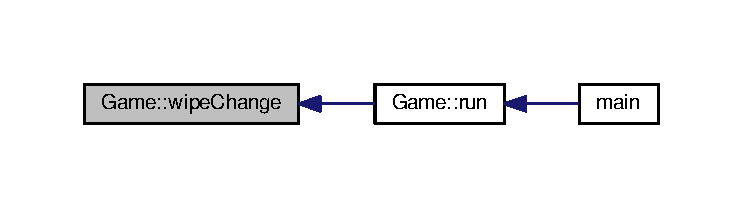
\includegraphics[width=350pt]{class_game_aa73688f1ba069a3f1989884099c58449_icgraph}
\end{center}
\end{figure}




\subsection{Member Data Documentation}
\hypertarget{class_game_a87f9c54e60a724de2644769cd917dbce}{\index{Game@{Game}!change@{change}}
\index{change@{change}!Game@{Game}}
\subsubsection[{change}]{\setlength{\rightskip}{0pt plus 5cm}{\bf Point}$\ast$ Game\-::change\mbox{[}2\mbox{]}\hspace{0.3cm}{\ttfamily [private]}}}\label{class_game_a87f9c54e60a724de2644769cd917dbce}


Definition at line 27 of file game.\-h.

\hypertarget{class_game_ae959d08e508fcef98dd07a2b9cd82e65}{\index{Game@{Game}!change\-Size@{change\-Size}}
\index{change\-Size@{change\-Size}!Game@{Game}}
\subsubsection[{change\-Size}]{\setlength{\rightskip}{0pt plus 5cm}int Game\-::change\-Size\hspace{0.3cm}{\ttfamily [private]}}}\label{class_game_ae959d08e508fcef98dd07a2b9cd82e65}


Definition at line 23 of file game.\-h.

\hypertarget{class_game_a92148f2659c019b331e9da7deadbd8bc}{\index{Game@{Game}!labyrinth@{labyrinth}}
\index{labyrinth@{labyrinth}!Game@{Game}}
\subsubsection[{labyrinth}]{\setlength{\rightskip}{0pt plus 5cm}{\bf Labyrinth} Game\-::labyrinth\hspace{0.3cm}{\ttfamily [private]}}}\label{class_game_a92148f2659c019b331e9da7deadbd8bc}


Definition at line 26 of file game.\-h.

\hypertarget{class_game_ab77bfcc312425811000819791ea7668e}{\index{Game@{Game}!snake@{snake}}
\index{snake@{snake}!Game@{Game}}
\subsubsection[{snake}]{\setlength{\rightskip}{0pt plus 5cm}{\bf Snake} Game\-::snake\hspace{0.3cm}{\ttfamily [private]}}}\label{class_game_ab77bfcc312425811000819791ea7668e}


Definition at line 24 of file game.\-h.

\hypertarget{class_game_ab7d2baa4a2dbcb64fc1611aac709fe40}{\index{Game@{Game}!snake\-Enemies@{snake\-Enemies}}
\index{snake\-Enemies@{snake\-Enemies}!Game@{Game}}
\subsubsection[{snake\-Enemies}]{\setlength{\rightskip}{0pt plus 5cm}{\bf Snake}$\ast$ Game\-::snake\-Enemies\hspace{0.3cm}{\ttfamily [private]}}}\label{class_game_ab7d2baa4a2dbcb64fc1611aac709fe40}


Definition at line 25 of file game.\-h.

\hypertarget{class_game_a02a58acc040d6d014e02832453695ef5}{\index{Game@{Game}!speed@{speed}}
\index{speed@{speed}!Game@{Game}}
\subsubsection[{speed}]{\setlength{\rightskip}{0pt plus 5cm}int Game\-::speed\hspace{0.3cm}{\ttfamily [private]}}}\label{class_game_a02a58acc040d6d014e02832453695ef5}


Definition at line 22 of file game.\-h.



The documentation for this class was generated from the following files\-:\begin{DoxyCompactItemize}
\item 
/home/travis/build/echo-\/team/\-Snoke/\-Libraries/\-Game/\hyperlink{game_8h}{game.\-h}\item 
/home/travis/build/echo-\/team/\-Snoke/\-Libraries/\-Game/\hyperlink{game_8cpp}{game.\-cpp}\end{DoxyCompactItemize}

\hypertarget{class_labyrinth}{\section{Labyrinth Class Reference}
\label{class_labyrinth}\index{Labyrinth@{Labyrinth}}
}


{\ttfamily \#include $<$labyrinth.\-h$>$}



Collaboration diagram for Labyrinth\-:
\nopagebreak
\begin{figure}[H]
\begin{center}
\leavevmode
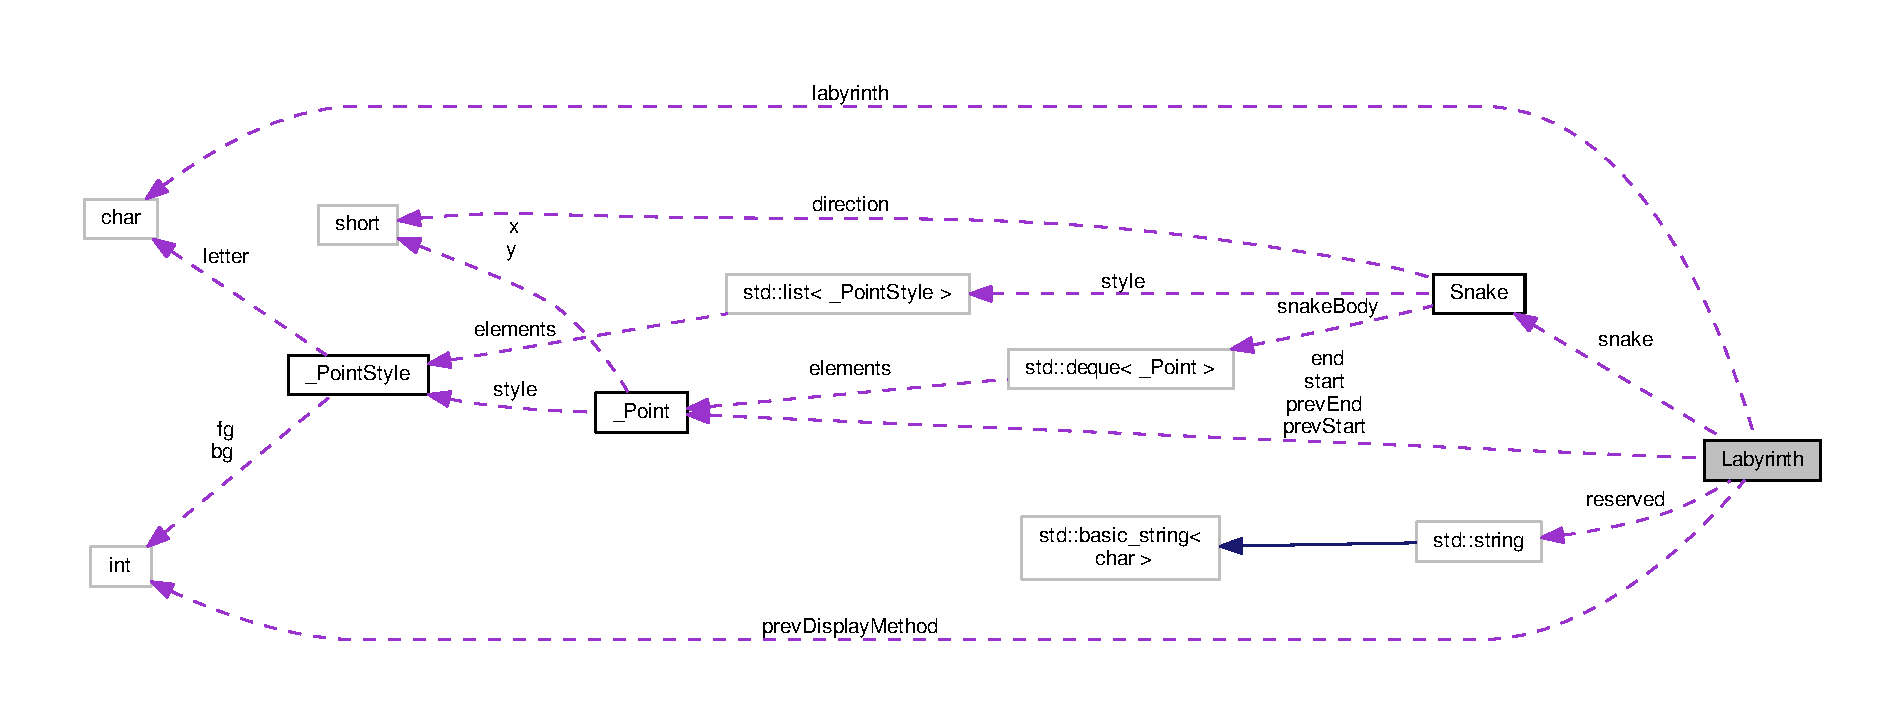
\includegraphics[width=350pt]{class_labyrinth__coll__graph}
\end{center}
\end{figure}
\subsection*{Public Member Functions}
\begin{DoxyCompactItemize}
\item 
void \hyperlink{class_labyrinth_a39e1b11a06d126328131d387fbf51d73}{set\-Labyrinth} (\hyperlink{common_8h_aa9cfdb80b4ca12013a2de8a3b9b97981}{Point} dimensions)
\item 
void \hyperlink{class_labyrinth_ad2819aba76d079c7fda751e7388b7182}{add\-Snake} (\hyperlink{class_snake}{Snake} $\ast$\hyperlink{class_labyrinth_a09a46368bfd83ccb75580687cb17b92f}{snake})
\item 
bool \hyperlink{class_labyrinth_a710cf4ff7789d527e6081d1eb2d696a6}{add\-Point} (\hyperlink{common_8h_aa9cfdb80b4ca12013a2de8a3b9b97981}{Point} p)
\item 
bool \hyperlink{class_labyrinth_a24d98083c011da23695425ec69d583a5}{rem\-Point} (\hyperlink{common_8h_aa9cfdb80b4ca12013a2de8a3b9b97981}{Point} p)
\item 
void \hyperlink{class_labyrinth_a02c42abb1b58fdf8a20b66bddd0bbe00}{display\-Handler} (\hyperlink{common_8h_aa9cfdb80b4ca12013a2de8a3b9b97981}{Point} $\ast$change\mbox{[}2\mbox{]}=N\-U\-L\-L, int size=0)
\item 
bool \hyperlink{class_labyrinth_acd7311e3222304bae2208fbc293bcc4d}{is\-Free} (\hyperlink{common_8h_aa9cfdb80b4ca12013a2de8a3b9b97981}{Point} p)
\item 
bool \hyperlink{class_labyrinth_a99e6b33f94d6d64f9c5a4fa78f08c007}{save} (char name\mbox{[}\hyperlink{common_8h_a3e937c42922f7601edb17b747602c471}{M\-A\-X\-L\-I\-N\-E}\mbox{]})
\item 
bool \hyperlink{class_labyrinth_a36cd7033292515cba0ce3d74f03720b6}{load} (char name\mbox{[}\hyperlink{common_8h_a3e937c42922f7601edb17b747602c471}{M\-A\-X\-L\-I\-N\-E}\mbox{]})
\end{DoxyCompactItemize}
\subsection*{Private Member Functions}
\begin{DoxyCompactItemize}
\item 
void \hyperlink{class_labyrinth_a676e53a7bced45343af8307eae2ba2d0}{display\-Labyrinth} ()
\item 
void \hyperlink{class_labyrinth_a86210707e3b4be4faaa9bd1f86429124}{display\-Updated} (\hyperlink{common_8h_aa9cfdb80b4ca12013a2de8a3b9b97981}{Point} $\ast$update\mbox{[}2\mbox{]}, int size)
\item 
void \hyperlink{class_labyrinth_ad533aaa69e845e368a7a08097f7e4ac8}{update\-Labyrinth} (\hyperlink{common_8h_aa9cfdb80b4ca12013a2de8a3b9b97981}{Point} $\ast$update\mbox{[}2\mbox{]}, int size)
\item 
void \hyperlink{class_labyrinth_a98447444cafe6d19e0e5c0181f3c1ddd}{display\-Full} ()
\item 
void \hyperlink{class_labyrinth_a43994d3b84ed457b1c04595466a61fc6}{size\-Handler} ()
\end{DoxyCompactItemize}
\subsection*{Private Attributes}
\begin{DoxyCompactItemize}
\item 
char $\ast$$\ast$ \hyperlink{class_labyrinth_ac95a1b4246b9351e8cea8c1618bcb58d}{labyrinth}
\item 
std\-::string \hyperlink{class_labyrinth_aafa921122b2ea77268cbe479949d7d39}{reserved} = \char`\"{}!\char`\"{}
\item 
int \hyperlink{class_labyrinth_a7ddef18e25e03408485e4959bcb5aebc}{prev\-Display\-Method} = 0
\item 
\hyperlink{class_snake}{Snake} $\ast$ \hyperlink{class_labyrinth_a09a46368bfd83ccb75580687cb17b92f}{snake} = N\-U\-L\-L
\item 
\hyperlink{common_8h_aa9cfdb80b4ca12013a2de8a3b9b97981}{Point} \hyperlink{class_labyrinth_a92649fa3b24fcc869418b54e7362e24f}{start}
\item 
\hyperlink{common_8h_aa9cfdb80b4ca12013a2de8a3b9b97981}{Point} \hyperlink{class_labyrinth_a5536b8752cb3c2ef273360e14224bc6f}{end}
\item 
\hyperlink{common_8h_aa9cfdb80b4ca12013a2de8a3b9b97981}{Point} \hyperlink{class_labyrinth_a23e08d55e3a627e8a0d828d05be03253}{prev\-Start}
\item 
\hyperlink{common_8h_aa9cfdb80b4ca12013a2de8a3b9b97981}{Point} \hyperlink{class_labyrinth_a9041d96d4328dea374deb81ff08bd35c}{prev\-End}
\end{DoxyCompactItemize}


\subsection{Detailed Description}
class for containing and siplaying the game field 
\begin{DoxyParams}{Parameters}
{\em \{char$\ast$$\ast$\}} & labyrinth -\/ game field, consisting of chars \\
\hline
{\em \{std\-::string\}} & reserved -\/ array of reserved chars for inside usage \\
\hline
{\em \{int\}} & prev\-Display\-Method -\/ value, containing the makr of which display method was previously called(is used in displaying) \\
\hline
{\em \{\-Snake$\ast$\}} & snake -\/ a pointer to a local\-\_\-player's snake  \{Point\} start -\/ a top left corner from which the drawing of the current cycle starts \\
\hline
{\em \{\-Point\}} & end -\/ a bottom right corner at which the drawing of the current cycle ends \\
\hline
\end{DoxyParams}


Definition at line 36 of file labyrinth.\-h.



\subsection{Member Function Documentation}
\hypertarget{class_labyrinth_a710cf4ff7789d527e6081d1eb2d696a6}{\index{Labyrinth@{Labyrinth}!add\-Point@{add\-Point}}
\index{add\-Point@{add\-Point}!Labyrinth@{Labyrinth}}
\subsubsection[{add\-Point}]{\setlength{\rightskip}{0pt plus 5cm}bool Labyrinth\-::add\-Point (
\begin{DoxyParamCaption}
\item[{{\bf Point}}]{p}
\end{DoxyParamCaption}
)}}\label{class_labyrinth_a710cf4ff7789d527e6081d1eb2d696a6}
Adding Point to the labyrinth with the check of correction 
\begin{DoxyParams}{Parameters}
{\em \{\-Point\}} & p -\/ point to add to the labyrinth \\
\hline
\end{DoxyParams}
\begin{DoxyReturn}{Returns}
\{bool\} -\/ mark of whether the Point was added 
\end{DoxyReturn}


Definition at line 267 of file labyrinth.\-cpp.



Here is the call graph for this function\-:
\nopagebreak
\begin{figure}[H]
\begin{center}
\leavevmode
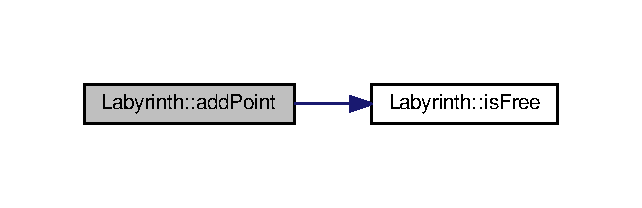
\includegraphics[width=308pt]{class_labyrinth_a710cf4ff7789d527e6081d1eb2d696a6_cgraph}
\end{center}
\end{figure}




Here is the caller graph for this function\-:
\nopagebreak
\begin{figure}[H]
\begin{center}
\leavevmode
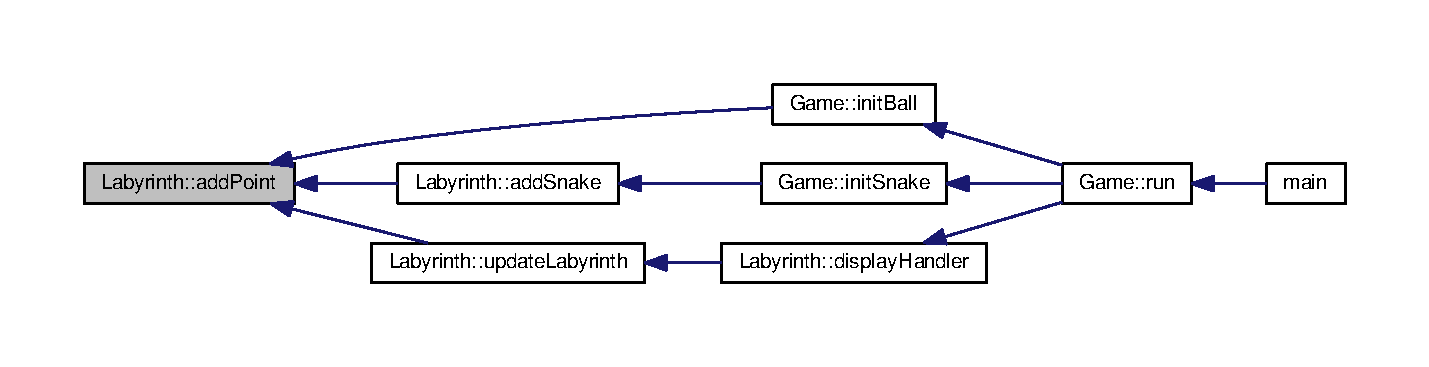
\includegraphics[width=350pt]{class_labyrinth_a710cf4ff7789d527e6081d1eb2d696a6_icgraph}
\end{center}
\end{figure}


\hypertarget{class_labyrinth_ad2819aba76d079c7fda751e7388b7182}{\index{Labyrinth@{Labyrinth}!add\-Snake@{add\-Snake}}
\index{add\-Snake@{add\-Snake}!Labyrinth@{Labyrinth}}
\subsubsection[{add\-Snake}]{\setlength{\rightskip}{0pt plus 5cm}void Labyrinth\-::add\-Snake (
\begin{DoxyParamCaption}
\item[{{\bf Snake} $\ast$}]{snake}
\end{DoxyParamCaption}
)}}\label{class_labyrinth_ad2819aba76d079c7fda751e7388b7182}
Adding snake to the laburinth and getting the host snake(firest added snake) 
\begin{DoxyParams}{Parameters}
{\em \{\-Snake$\ast$\}} & snake -\/ a snake to add \\
\hline
\end{DoxyParams}


Definition at line 50 of file labyrinth.\-cpp.



Here is the call graph for this function\-:
\nopagebreak
\begin{figure}[H]
\begin{center}
\leavevmode
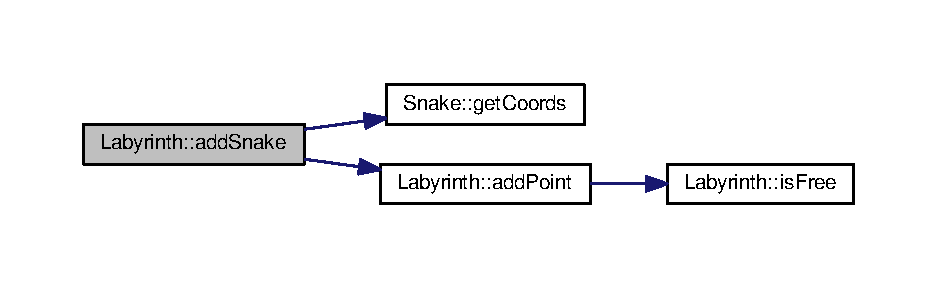
\includegraphics[width=350pt]{class_labyrinth_ad2819aba76d079c7fda751e7388b7182_cgraph}
\end{center}
\end{figure}




Here is the caller graph for this function\-:
\nopagebreak
\begin{figure}[H]
\begin{center}
\leavevmode
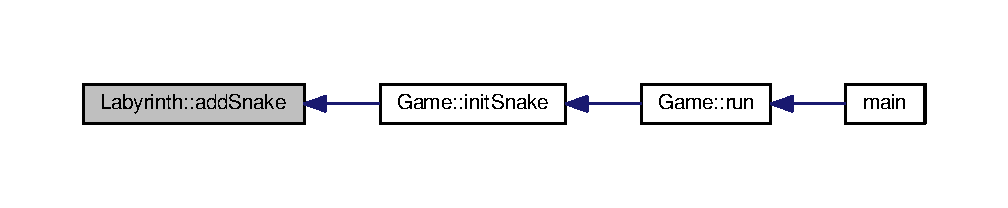
\includegraphics[width=350pt]{class_labyrinth_ad2819aba76d079c7fda751e7388b7182_icgraph}
\end{center}
\end{figure}


\hypertarget{class_labyrinth_a98447444cafe6d19e0e5c0181f3c1ddd}{\index{Labyrinth@{Labyrinth}!display\-Full@{display\-Full}}
\index{display\-Full@{display\-Full}!Labyrinth@{Labyrinth}}
\subsubsection[{display\-Full}]{\setlength{\rightskip}{0pt plus 5cm}void Labyrinth\-::display\-Full (
\begin{DoxyParamCaption}
{}
\end{DoxyParamCaption}
)\hspace{0.3cm}{\ttfamily [private]}}}\label{class_labyrinth_a98447444cafe6d19e0e5c0181f3c1ddd}
redraw every Point of the labyrinth 

Definition at line 187 of file labyrinth.\-cpp.



Here is the caller graph for this function\-:
\nopagebreak
\begin{figure}[H]
\begin{center}
\leavevmode
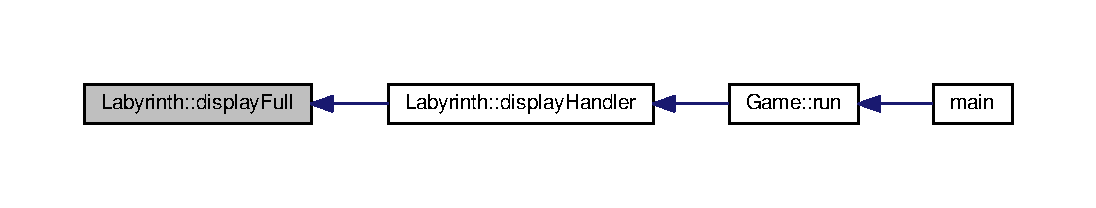
\includegraphics[width=350pt]{class_labyrinth_a98447444cafe6d19e0e5c0181f3c1ddd_icgraph}
\end{center}
\end{figure}


\hypertarget{class_labyrinth_a02c42abb1b58fdf8a20b66bddd0bbe00}{\index{Labyrinth@{Labyrinth}!display\-Handler@{display\-Handler}}
\index{display\-Handler@{display\-Handler}!Labyrinth@{Labyrinth}}
\subsubsection[{display\-Handler}]{\setlength{\rightskip}{0pt plus 5cm}void Labyrinth\-::display\-Handler (
\begin{DoxyParamCaption}
\item[{{\bf Point} $\ast$}]{change\mbox{[}2\mbox{]} = {\ttfamily NULL}, }
\item[{int}]{size = {\ttfamily 0}}
\end{DoxyParamCaption}
)}}\label{class_labyrinth_a02c42abb1b58fdf8a20b66bddd0bbe00}
A method which decides what dispaly method will be used in each situation 
\begin{DoxyParams}{Parameters}
{\em \{\-Point$\ast$\}} & change -\/ 2-\/dimensional array of changes needed to be applied to the labyrinth \\
\hline
{\em \{int\}} & size -\/ the size of the change array \\
\hline
\end{DoxyParams}


Definition at line 68 of file labyrinth.\-cpp.



Here is the call graph for this function\-:
\nopagebreak
\begin{figure}[H]
\begin{center}
\leavevmode
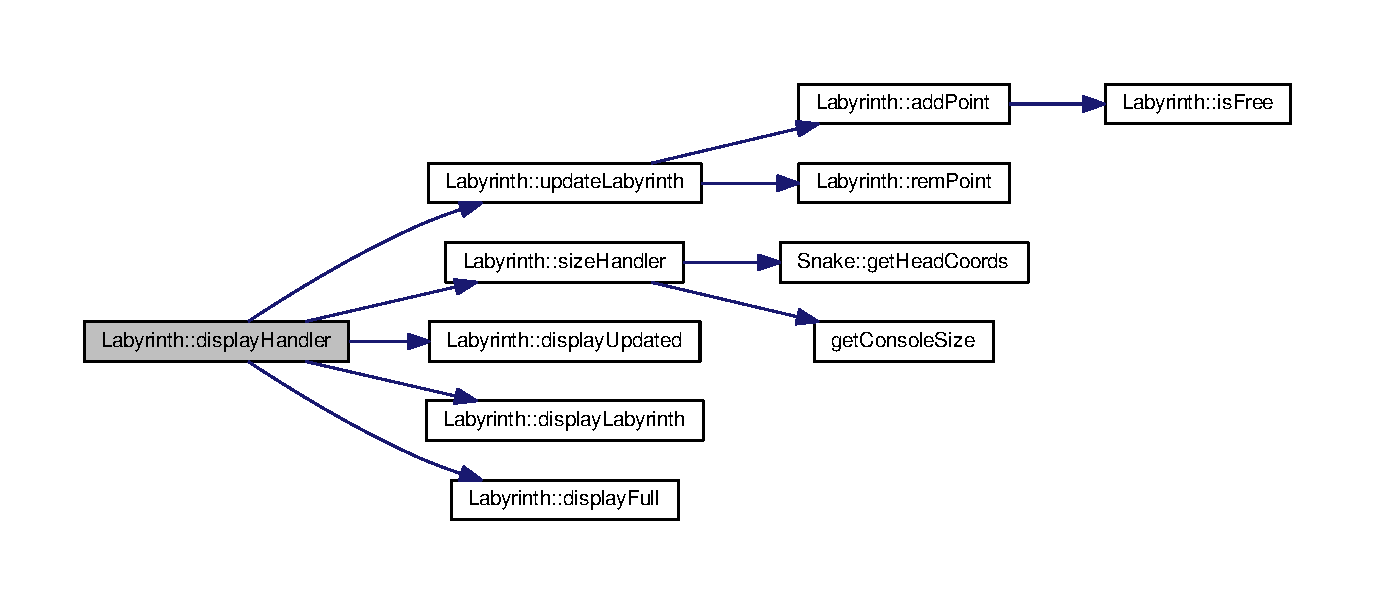
\includegraphics[width=350pt]{class_labyrinth_a02c42abb1b58fdf8a20b66bddd0bbe00_cgraph}
\end{center}
\end{figure}




Here is the caller graph for this function\-:
\nopagebreak
\begin{figure}[H]
\begin{center}
\leavevmode
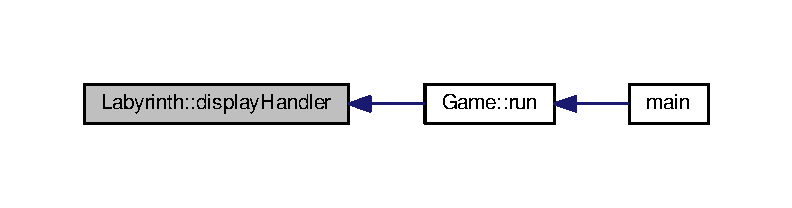
\includegraphics[width=350pt]{class_labyrinth_a02c42abb1b58fdf8a20b66bddd0bbe00_icgraph}
\end{center}
\end{figure}


\hypertarget{class_labyrinth_a676e53a7bced45343af8307eae2ba2d0}{\index{Labyrinth@{Labyrinth}!display\-Labyrinth@{display\-Labyrinth}}
\index{display\-Labyrinth@{display\-Labyrinth}!Labyrinth@{Labyrinth}}
\subsubsection[{display\-Labyrinth}]{\setlength{\rightskip}{0pt plus 5cm}void Labyrinth\-::display\-Labyrinth (
\begin{DoxyParamCaption}
{}
\end{DoxyParamCaption}
)\hspace{0.3cm}{\ttfamily [private]}}}\label{class_labyrinth_a676e53a7bced45343af8307eae2ba2d0}
display labyrinth partialy, using the start and end Points 

Definition at line 199 of file labyrinth.\-cpp.



Here is the caller graph for this function\-:
\nopagebreak
\begin{figure}[H]
\begin{center}
\leavevmode
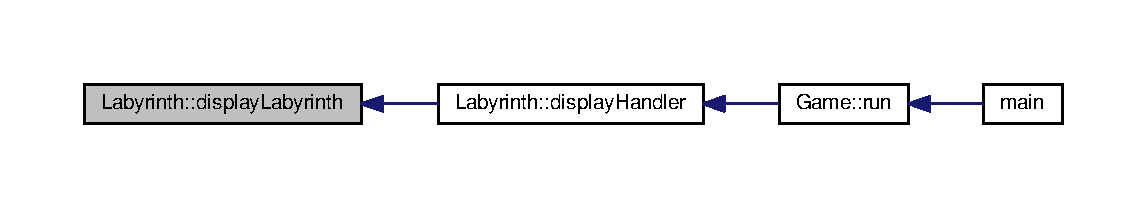
\includegraphics[width=350pt]{class_labyrinth_a676e53a7bced45343af8307eae2ba2d0_icgraph}
\end{center}
\end{figure}


\hypertarget{class_labyrinth_a86210707e3b4be4faaa9bd1f86429124}{\index{Labyrinth@{Labyrinth}!display\-Updated@{display\-Updated}}
\index{display\-Updated@{display\-Updated}!Labyrinth@{Labyrinth}}
\subsubsection[{display\-Updated}]{\setlength{\rightskip}{0pt plus 5cm}void Labyrinth\-::display\-Updated (
\begin{DoxyParamCaption}
\item[{{\bf Point} $\ast$}]{update\mbox{[}2\mbox{]}, }
\item[{int}]{size}
\end{DoxyParamCaption}
)\hspace{0.3cm}{\ttfamily [private]}}}\label{class_labyrinth_a86210707e3b4be4faaa9bd1f86429124}
draw only the changed Points when the labyrinth is being fully displayed 

Definition at line 216 of file labyrinth.\-cpp.



Here is the caller graph for this function\-:
\nopagebreak
\begin{figure}[H]
\begin{center}
\leavevmode
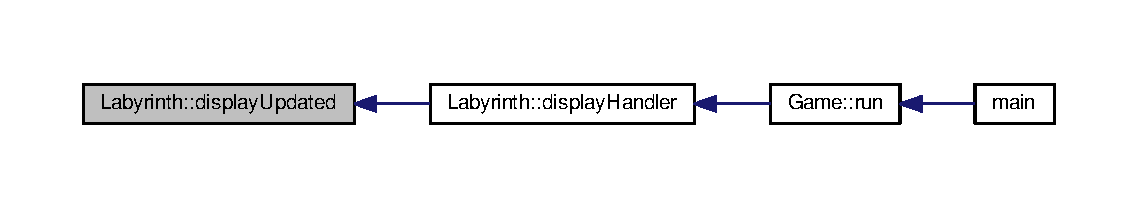
\includegraphics[width=350pt]{class_labyrinth_a86210707e3b4be4faaa9bd1f86429124_icgraph}
\end{center}
\end{figure}


\hypertarget{class_labyrinth_acd7311e3222304bae2208fbc293bcc4d}{\index{Labyrinth@{Labyrinth}!is\-Free@{is\-Free}}
\index{is\-Free@{is\-Free}!Labyrinth@{Labyrinth}}
\subsubsection[{is\-Free}]{\setlength{\rightskip}{0pt plus 5cm}bool Labyrinth\-::is\-Free (
\begin{DoxyParamCaption}
\item[{{\bf Point}}]{p}
\end{DoxyParamCaption}
)}}\label{class_labyrinth_acd7311e3222304bae2208fbc293bcc4d}
Mark of if the asked Point is free 
\begin{DoxyParams}{Parameters}
{\em \{\-Point\}} & p -\/ Point to check in the labyrinth \\
\hline
\end{DoxyParams}
\begin{DoxyReturn}{Returns}
\{bool\} -\/ mark of whether the Point is free 
\end{DoxyReturn}


Definition at line 257 of file labyrinth.\-cpp.



Here is the caller graph for this function\-:
\nopagebreak
\begin{figure}[H]
\begin{center}
\leavevmode
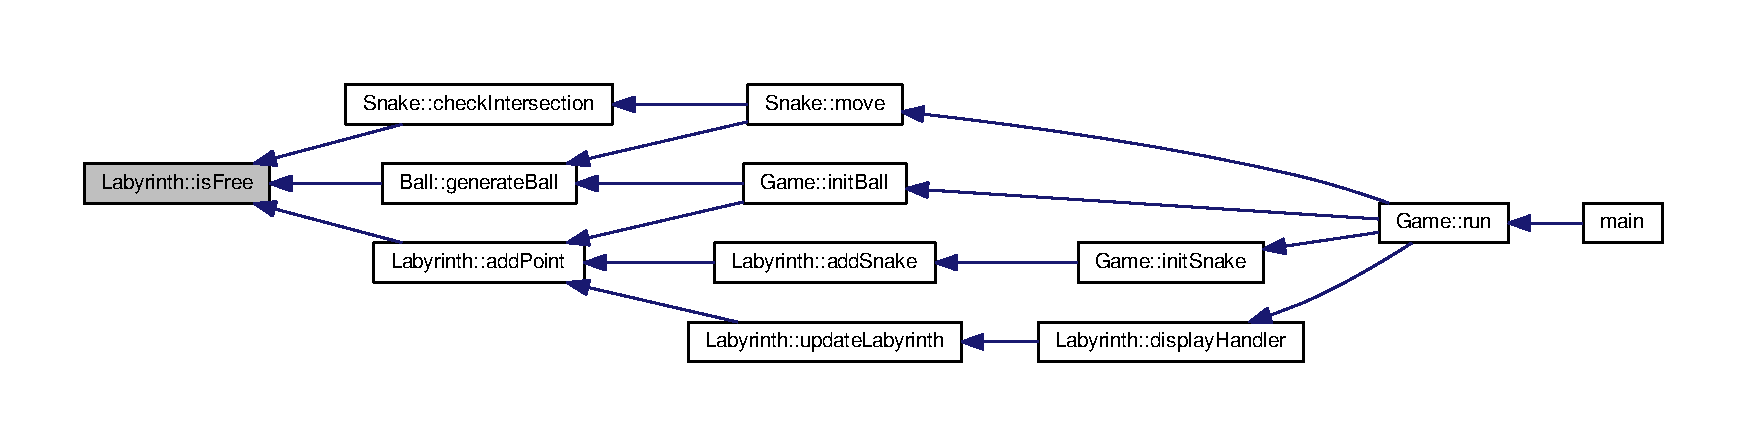
\includegraphics[width=350pt]{class_labyrinth_acd7311e3222304bae2208fbc293bcc4d_icgraph}
\end{center}
\end{figure}


\hypertarget{class_labyrinth_a36cd7033292515cba0ce3d74f03720b6}{\index{Labyrinth@{Labyrinth}!load@{load}}
\index{load@{load}!Labyrinth@{Labyrinth}}
\subsubsection[{load}]{\setlength{\rightskip}{0pt plus 5cm}bool Labyrinth\-::load (
\begin{DoxyParamCaption}
\item[{char}]{name\mbox{[}\-M\-A\-X\-L\-I\-N\-E\mbox{]}}
\end{DoxyParamCaption}
)}}\label{class_labyrinth_a36cd7033292515cba0ce3d74f03720b6}
Mehod to load labyrinth from the file 
\begin{DoxyParams}{Parameters}
{\em \{char$\ast$\}} & name -\/ name of the file to read from \\
\hline
\end{DoxyParams}
\begin{DoxyReturn}{Returns}
\{bool\} -\/ mark os successful loading 
\end{DoxyReturn}


Definition at line 335 of file labyrinth.\-cpp.



Here is the caller graph for this function\-:
\nopagebreak
\begin{figure}[H]
\begin{center}
\leavevmode
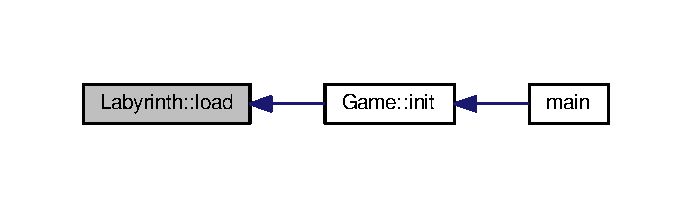
\includegraphics[width=332pt]{class_labyrinth_a36cd7033292515cba0ce3d74f03720b6_icgraph}
\end{center}
\end{figure}


\hypertarget{class_labyrinth_a24d98083c011da23695425ec69d583a5}{\index{Labyrinth@{Labyrinth}!rem\-Point@{rem\-Point}}
\index{rem\-Point@{rem\-Point}!Labyrinth@{Labyrinth}}
\subsubsection[{rem\-Point}]{\setlength{\rightskip}{0pt plus 5cm}bool Labyrinth\-::rem\-Point (
\begin{DoxyParamCaption}
\item[{{\bf Point}}]{p}
\end{DoxyParamCaption}
)}}\label{class_labyrinth_a24d98083c011da23695425ec69d583a5}
Remove Point from the labyrinth 
\begin{DoxyParams}{Parameters}
{\em \{\-Point\}} & p -\/ point to remove from the labyrinth \\
\hline
\end{DoxyParams}
\begin{DoxyReturn}{Returns}
\{bool\} -\/ mark of whether the Point was removed 
\end{DoxyReturn}


Definition at line 282 of file labyrinth.\-cpp.



Here is the caller graph for this function\-:
\nopagebreak
\begin{figure}[H]
\begin{center}
\leavevmode
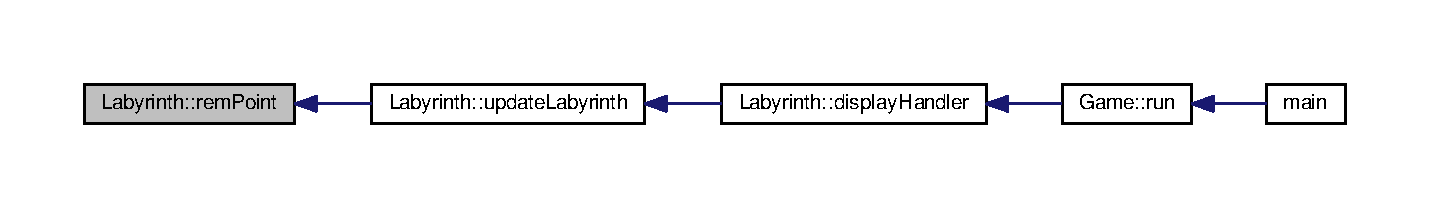
\includegraphics[width=350pt]{class_labyrinth_a24d98083c011da23695425ec69d583a5_icgraph}
\end{center}
\end{figure}


\hypertarget{class_labyrinth_a99e6b33f94d6d64f9c5a4fa78f08c007}{\index{Labyrinth@{Labyrinth}!save@{save}}
\index{save@{save}!Labyrinth@{Labyrinth}}
\subsubsection[{save}]{\setlength{\rightskip}{0pt plus 5cm}bool Labyrinth\-::save (
\begin{DoxyParamCaption}
\item[{char}]{name\mbox{[}\-M\-A\-X\-L\-I\-N\-E\mbox{]}}
\end{DoxyParamCaption}
)}}\label{class_labyrinth_a99e6b33f94d6d64f9c5a4fa78f08c007}
Method to save labyritnh(borders and obstacles, defined in reserved string) to the file 
\begin{DoxyParams}{Parameters}
{\em \{char$\ast$\}} & name -\/ name of the file, where to sace the labyrinth \\
\hline
\end{DoxyParams}
\begin{DoxyReturn}{Returns}
\{bool\} -\/ mark of whether the labyrinth was successfully saved 
\end{DoxyReturn}


Definition at line 293 of file labyrinth.\-cpp.



Here is the caller graph for this function\-:
\nopagebreak
\begin{figure}[H]
\begin{center}
\leavevmode
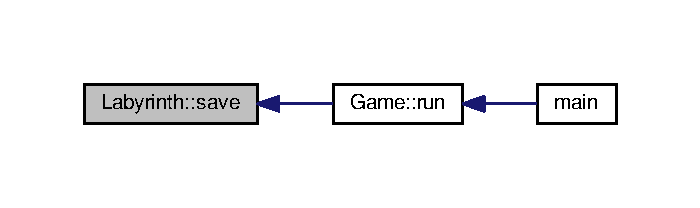
\includegraphics[width=336pt]{class_labyrinth_a99e6b33f94d6d64f9c5a4fa78f08c007_icgraph}
\end{center}
\end{figure}


\hypertarget{class_labyrinth_a39e1b11a06d126328131d387fbf51d73}{\index{Labyrinth@{Labyrinth}!set\-Labyrinth@{set\-Labyrinth}}
\index{set\-Labyrinth@{set\-Labyrinth}!Labyrinth@{Labyrinth}}
\subsubsection[{set\-Labyrinth}]{\setlength{\rightskip}{0pt plus 5cm}void Labyrinth\-::set\-Labyrinth (
\begin{DoxyParamCaption}
\item[{{\bf Point}}]{game\-Field\-Size}
\end{DoxyParamCaption}
)}}\label{class_labyrinth_a39e1b11a06d126328131d387fbf51d73}
Sets the default values fro the variables as well as generating the labyritnh array with borders 
\begin{DoxyParams}{Parameters}
{\em \{\-Point\}} & game\-Field\-Size -\/ a size of the labyrinth \\
\hline
\end{DoxyParams}


Definition at line 6 of file labyrinth.\-cpp.



Here is the caller graph for this function\-:
\nopagebreak
\begin{figure}[H]
\begin{center}
\leavevmode
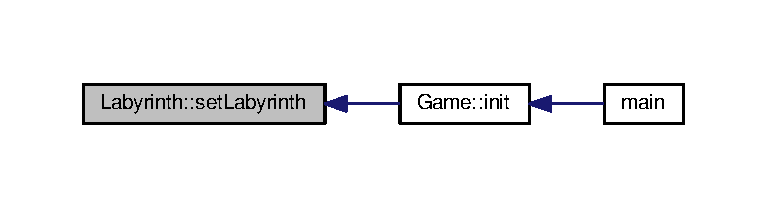
\includegraphics[width=350pt]{class_labyrinth_a39e1b11a06d126328131d387fbf51d73_icgraph}
\end{center}
\end{figure}


\hypertarget{class_labyrinth_a43994d3b84ed457b1c04595466a61fc6}{\index{Labyrinth@{Labyrinth}!size\-Handler@{size\-Handler}}
\index{size\-Handler@{size\-Handler}!Labyrinth@{Labyrinth}}
\subsubsection[{size\-Handler}]{\setlength{\rightskip}{0pt plus 5cm}void Labyrinth\-::size\-Handler (
\begin{DoxyParamCaption}
{}
\end{DoxyParamCaption}
)\hspace{0.3cm}{\ttfamily [private]}}}\label{class_labyrinth_a43994d3b84ed457b1c04595466a61fc6}
A method, which sets start and end values depending on the position of local\-\_\-player's snake head and current console size 

Definition at line 127 of file labyrinth.\-cpp.



Here is the call graph for this function\-:
\nopagebreak
\begin{figure}[H]
\begin{center}
\leavevmode
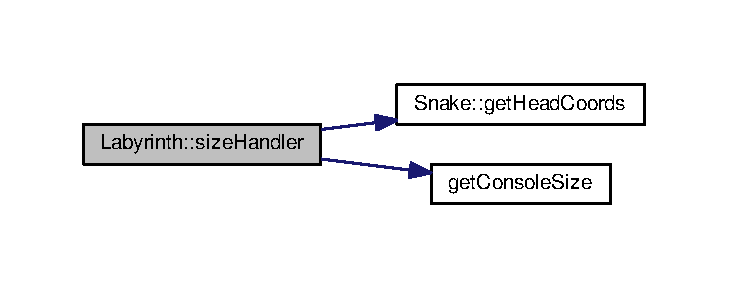
\includegraphics[width=350pt]{class_labyrinth_a43994d3b84ed457b1c04595466a61fc6_cgraph}
\end{center}
\end{figure}




Here is the caller graph for this function\-:
\nopagebreak
\begin{figure}[H]
\begin{center}
\leavevmode
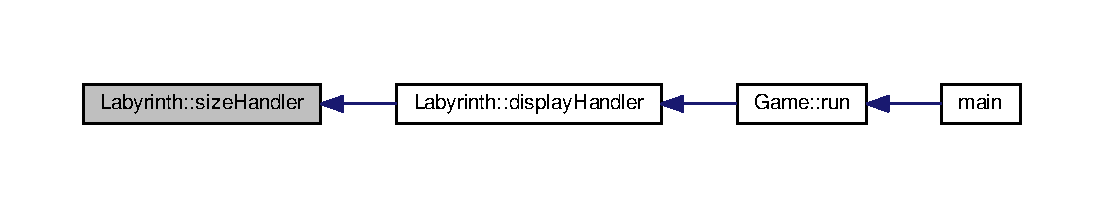
\includegraphics[width=350pt]{class_labyrinth_a43994d3b84ed457b1c04595466a61fc6_icgraph}
\end{center}
\end{figure}


\hypertarget{class_labyrinth_ad533aaa69e845e368a7a08097f7e4ac8}{\index{Labyrinth@{Labyrinth}!update\-Labyrinth@{update\-Labyrinth}}
\index{update\-Labyrinth@{update\-Labyrinth}!Labyrinth@{Labyrinth}}
\subsubsection[{update\-Labyrinth}]{\setlength{\rightskip}{0pt plus 5cm}void Labyrinth\-::update\-Labyrinth (
\begin{DoxyParamCaption}
\item[{{\bf Point} $\ast$}]{update\mbox{[}2\mbox{]}, }
\item[{int}]{size}
\end{DoxyParamCaption}
)\hspace{0.3cm}{\ttfamily [private]}}}\label{class_labyrinth_ad533aaa69e845e368a7a08097f7e4ac8}
Updating the labyrinth(changing the values of some Points) 
\begin{DoxyParams}{Parameters}
{\em \{\-Point$\ast$\}} & update -\/ 2-\/dimensional array of changes needed to be applied to the labyrinth \\
\hline
{\em \{int\}} & size -\/ the longest sequence for updating \mbox{[}max(len(update\mbox{[}0\mbox{]}, update\mbox{[}1\mbox{]}))\mbox{]} \\
\hline
\end{DoxyParams}


Definition at line 234 of file labyrinth.\-cpp.



Here is the call graph for this function\-:
\nopagebreak
\begin{figure}[H]
\begin{center}
\leavevmode
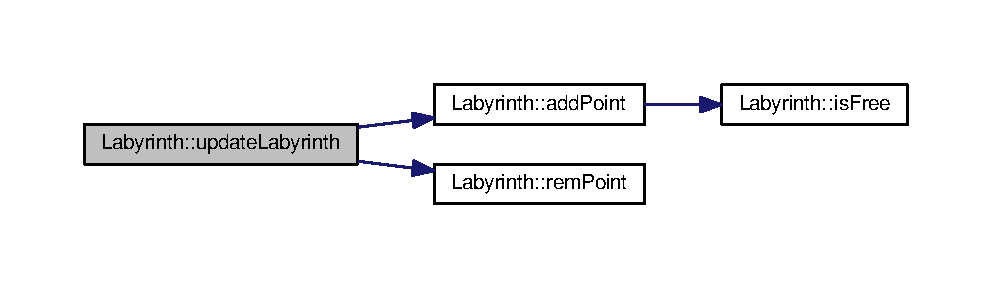
\includegraphics[width=350pt]{class_labyrinth_ad533aaa69e845e368a7a08097f7e4ac8_cgraph}
\end{center}
\end{figure}




Here is the caller graph for this function\-:
\nopagebreak
\begin{figure}[H]
\begin{center}
\leavevmode
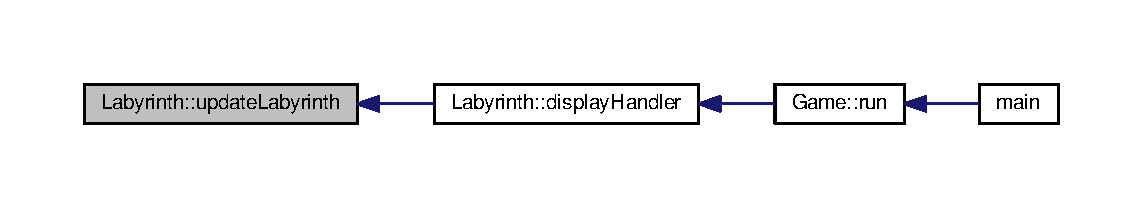
\includegraphics[width=350pt]{class_labyrinth_ad533aaa69e845e368a7a08097f7e4ac8_icgraph}
\end{center}
\end{figure}




\subsection{Member Data Documentation}
\hypertarget{class_labyrinth_a5536b8752cb3c2ef273360e14224bc6f}{\index{Labyrinth@{Labyrinth}!end@{end}}
\index{end@{end}!Labyrinth@{Labyrinth}}
\subsubsection[{end}]{\setlength{\rightskip}{0pt plus 5cm}{\bf Point} Labyrinth\-::end\hspace{0.3cm}{\ttfamily [private]}}}\label{class_labyrinth_a5536b8752cb3c2ef273360e14224bc6f}


Definition at line 44 of file labyrinth.\-h.

\hypertarget{class_labyrinth_ac95a1b4246b9351e8cea8c1618bcb58d}{\index{Labyrinth@{Labyrinth}!labyrinth@{labyrinth}}
\index{labyrinth@{labyrinth}!Labyrinth@{Labyrinth}}
\subsubsection[{labyrinth}]{\setlength{\rightskip}{0pt plus 5cm}char$\ast$$\ast$ Labyrinth\-::labyrinth\hspace{0.3cm}{\ttfamily [private]}}}\label{class_labyrinth_ac95a1b4246b9351e8cea8c1618bcb58d}


Definition at line 39 of file labyrinth.\-h.

\hypertarget{class_labyrinth_a7ddef18e25e03408485e4959bcb5aebc}{\index{Labyrinth@{Labyrinth}!prev\-Display\-Method@{prev\-Display\-Method}}
\index{prev\-Display\-Method@{prev\-Display\-Method}!Labyrinth@{Labyrinth}}
\subsubsection[{prev\-Display\-Method}]{\setlength{\rightskip}{0pt plus 5cm}int Labyrinth\-::prev\-Display\-Method = 0\hspace{0.3cm}{\ttfamily [private]}}}\label{class_labyrinth_a7ddef18e25e03408485e4959bcb5aebc}


Definition at line 41 of file labyrinth.\-h.

\hypertarget{class_labyrinth_a9041d96d4328dea374deb81ff08bd35c}{\index{Labyrinth@{Labyrinth}!prev\-End@{prev\-End}}
\index{prev\-End@{prev\-End}!Labyrinth@{Labyrinth}}
\subsubsection[{prev\-End}]{\setlength{\rightskip}{0pt plus 5cm}{\bf Point} Labyrinth\-::prev\-End\hspace{0.3cm}{\ttfamily [private]}}}\label{class_labyrinth_a9041d96d4328dea374deb81ff08bd35c}


Definition at line 46 of file labyrinth.\-h.

\hypertarget{class_labyrinth_a23e08d55e3a627e8a0d828d05be03253}{\index{Labyrinth@{Labyrinth}!prev\-Start@{prev\-Start}}
\index{prev\-Start@{prev\-Start}!Labyrinth@{Labyrinth}}
\subsubsection[{prev\-Start}]{\setlength{\rightskip}{0pt plus 5cm}{\bf Point} Labyrinth\-::prev\-Start\hspace{0.3cm}{\ttfamily [private]}}}\label{class_labyrinth_a23e08d55e3a627e8a0d828d05be03253}


Definition at line 45 of file labyrinth.\-h.

\hypertarget{class_labyrinth_aafa921122b2ea77268cbe479949d7d39}{\index{Labyrinth@{Labyrinth}!reserved@{reserved}}
\index{reserved@{reserved}!Labyrinth@{Labyrinth}}
\subsubsection[{reserved}]{\setlength{\rightskip}{0pt plus 5cm}std\-::string Labyrinth\-::reserved = \char`\"{}!\char`\"{}\hspace{0.3cm}{\ttfamily [private]}}}\label{class_labyrinth_aafa921122b2ea77268cbe479949d7d39}


Definition at line 40 of file labyrinth.\-h.

\hypertarget{class_labyrinth_a09a46368bfd83ccb75580687cb17b92f}{\index{Labyrinth@{Labyrinth}!snake@{snake}}
\index{snake@{snake}!Labyrinth@{Labyrinth}}
\subsubsection[{snake}]{\setlength{\rightskip}{0pt plus 5cm}{\bf Snake}$\ast$ Labyrinth\-::snake = N\-U\-L\-L\hspace{0.3cm}{\ttfamily [private]}}}\label{class_labyrinth_a09a46368bfd83ccb75580687cb17b92f}


Definition at line 42 of file labyrinth.\-h.

\hypertarget{class_labyrinth_a92649fa3b24fcc869418b54e7362e24f}{\index{Labyrinth@{Labyrinth}!start@{start}}
\index{start@{start}!Labyrinth@{Labyrinth}}
\subsubsection[{start}]{\setlength{\rightskip}{0pt plus 5cm}{\bf Point} Labyrinth\-::start\hspace{0.3cm}{\ttfamily [private]}}}\label{class_labyrinth_a92649fa3b24fcc869418b54e7362e24f}


Definition at line 43 of file labyrinth.\-h.



The documentation for this class was generated from the following files\-:\begin{DoxyCompactItemize}
\item 
/home/travis/build/echo-\/team/\-Snoke/\-Libraries/\-Labyrinth/\hyperlink{labyrinth_8h}{labyrinth.\-h}\item 
/home/travis/build/echo-\/team/\-Snoke/\-Libraries/\-Labyrinth/\hyperlink{labyrinth_8cpp}{labyrinth.\-cpp}\end{DoxyCompactItemize}

\hypertarget{class_logo}{}\section{Logo Class Reference}
\label{class_logo}\index{Logo@{Logo}}


{\ttfamily \#include $<$logo.\+h$>$}



Collaboration diagram for Logo\+:
\nopagebreak
\begin{figure}[H]
\begin{center}
\leavevmode
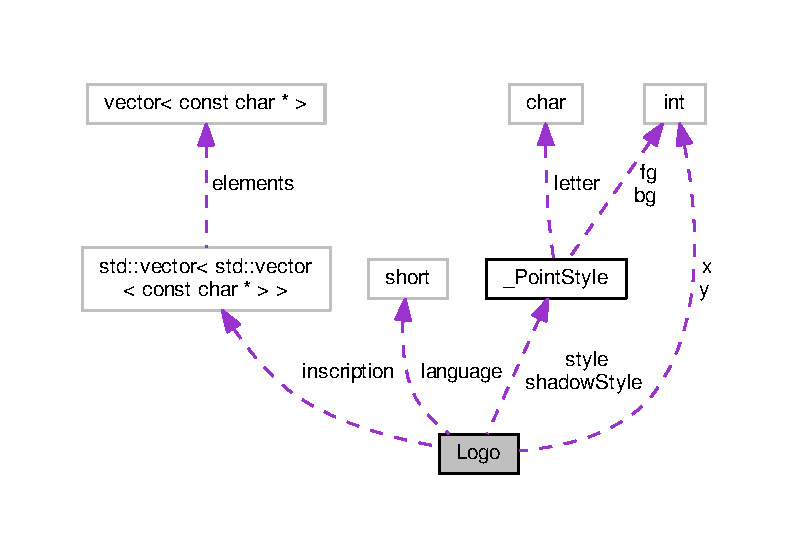
\includegraphics[width=350pt]{class_logo__coll__graph}
\end{center}
\end{figure}
\subsection*{Public Member Functions}
\begin{DoxyCompactItemize}
\item 
void \mbox{\hyperlink{class_logo_aced3f5817a709bcc0fd7cf8a360a2523}{draw}} ()
\item 
void \mbox{\hyperlink{class_logo_a048b9474c23e659c94f590509376f198}{set\+Position}} (int \mbox{\hyperlink{class_logo_ab25a813d9b3635c4b524dab9bc2ee86e}{x}}, int \mbox{\hyperlink{class_logo_a33846b1b3ac0da8180c888fb9a1680f6}{y}})
\item 
\mbox{\hyperlink{common_8h_aa9cfdb80b4ca12013a2de8a3b9b97981}{Point}} \mbox{\hyperlink{class_logo_aeeefce0ee601c896c38b929b7a355616}{get\+Size}} ()
\item 
\mbox{\hyperlink{class_logo_a1cdb59eff67441b73e9d0450e6a88921}{Logo}} (int \mbox{\hyperlink{class_logo_ab25a813d9b3635c4b524dab9bc2ee86e}{x}}, int \mbox{\hyperlink{class_logo_a33846b1b3ac0da8180c888fb9a1680f6}{y}}, \mbox{\hyperlink{common_8h_afd9cb36d6ef309c77ea1e3177e19c623}{Point\+Style}} \mbox{\hyperlink{class_logo_a2a0115dd4566f475c108eb3728265b62}{style}}, \mbox{\hyperlink{common_8h_afd9cb36d6ef309c77ea1e3177e19c623}{Point\+Style}} \mbox{\hyperlink{class_logo_a73d851ecd0cf3b7513f47df2aa462142}{shadow\+Style}}, int \mbox{\hyperlink{class_logo_ac3f13aa3fd16b904a71157e6ff47e48e}{language}})
\end{DoxyCompactItemize}
\subsection*{Private Attributes}
\begin{DoxyCompactItemize}
\item 
int \mbox{\hyperlink{class_logo_ab25a813d9b3635c4b524dab9bc2ee86e}{x}}
\item 
int \mbox{\hyperlink{class_logo_a33846b1b3ac0da8180c888fb9a1680f6}{y}}
\item 
\mbox{\hyperlink{common_8h_afd9cb36d6ef309c77ea1e3177e19c623}{Point\+Style}} \mbox{\hyperlink{class_logo_a2a0115dd4566f475c108eb3728265b62}{style}}
\item 
\mbox{\hyperlink{common_8h_afd9cb36d6ef309c77ea1e3177e19c623}{Point\+Style}} \mbox{\hyperlink{class_logo_a73d851ecd0cf3b7513f47df2aa462142}{shadow\+Style}}
\item 
short \mbox{\hyperlink{class_logo_ac3f13aa3fd16b904a71157e6ff47e48e}{language}}
\item 
std\+::vector$<$ std\+::vector$<$ const char $\ast$ $>$ $>$ \mbox{\hyperlink{class_logo_aefd60c44e3a7b4648e9758117db11244}{inscription}}
\end{DoxyCompactItemize}


\subsection{Detailed Description}
Class of the giant snoke logo 
\begin{DoxyParams}{Parameters}
{\em \{int\}} & x -\/ x coordinate of left logo side \\
\hline
{\em \{int\}} & y -\/ y coordinate of top logo side \\
\hline
{\em \{\+Point\+Style\}} & style -\/ style of the cells with logo \\
\hline
{\em \{\+Point\+Style\}} & shadow\+Style -\/ style of the cells with shadow of the logo \\
\hline
{\em \{short\}} & language -\/ language of the inscription at the logo, 0 -\/ en, 1 -\/ ru \\
\hline
{\em \{map$<$short,const} & char$\ast$$>$\} inscription -\/ dictionary with translations for inscription \\
\hline
\end{DoxyParams}


Definition at line 17 of file logo.\+h.



\subsection{Constructor \& Destructor Documentation}
\mbox{\Hypertarget{class_logo_a1cdb59eff67441b73e9d0450e6a88921}\label{class_logo_a1cdb59eff67441b73e9d0450e6a88921}} 
\index{Logo@{Logo}!Logo@{Logo}}
\index{Logo@{Logo}!Logo@{Logo}}
\subsubsection{\texorpdfstring{Logo()}{Logo()}}
{\footnotesize\ttfamily Logo\+::\+Logo (\begin{DoxyParamCaption}\item[{int}]{x,  }\item[{int}]{y,  }\item[{\mbox{\hyperlink{common_8h_afd9cb36d6ef309c77ea1e3177e19c623}{Point\+Style}}}]{style,  }\item[{\mbox{\hyperlink{common_8h_afd9cb36d6ef309c77ea1e3177e19c623}{Point\+Style}}}]{shadow\+Style,  }\item[{int}]{language }\end{DoxyParamCaption})}

@constructor 
\begin{DoxyParams}{Parameters}
{\em \{\+Point\+Style\}} & style -\/ style of the cells with logo \\
\hline
{\em \{\+Point\+Style\}} & shadow\+Style -\/ style of the cells with shadow of the logo \\
\hline
\end{DoxyParams}


Definition at line 61 of file logo.\+cpp.



\subsection{Member Function Documentation}
\mbox{\Hypertarget{class_logo_aced3f5817a709bcc0fd7cf8a360a2523}\label{class_logo_aced3f5817a709bcc0fd7cf8a360a2523}} 
\index{Logo@{Logo}!draw@{draw}}
\index{draw@{draw}!Logo@{Logo}}
\subsubsection{\texorpdfstring{draw()}{draw()}}
{\footnotesize\ttfamily void Logo\+::draw (\begin{DoxyParamCaption}{ }\end{DoxyParamCaption})}

Draws \mbox{\hyperlink{class_logo}{Logo}} in console window 

Definition at line 30 of file logo.\+cpp.

\mbox{\Hypertarget{class_logo_aeeefce0ee601c896c38b929b7a355616}\label{class_logo_aeeefce0ee601c896c38b929b7a355616}} 
\index{Logo@{Logo}!getSize@{getSize}}
\index{getSize@{getSize}!Logo@{Logo}}
\subsubsection{\texorpdfstring{getSize()}{getSize()}}
{\footnotesize\ttfamily \mbox{\hyperlink{common_8h_aa9cfdb80b4ca12013a2de8a3b9b97981}{Point}} Logo\+::get\+Size (\begin{DoxyParamCaption}{ }\end{DoxyParamCaption})}

Returns size of the logo \begin{DoxyReturn}{Returns}
\{Point\} -\/ width and height of the logo 
\end{DoxyReturn}


Definition at line 18 of file logo.\+cpp.

\mbox{\Hypertarget{class_logo_a048b9474c23e659c94f590509376f198}\label{class_logo_a048b9474c23e659c94f590509376f198}} 
\index{Logo@{Logo}!setPosition@{setPosition}}
\index{setPosition@{setPosition}!Logo@{Logo}}
\subsubsection{\texorpdfstring{setPosition()}{setPosition()}}
{\footnotesize\ttfamily void Logo\+::set\+Position (\begin{DoxyParamCaption}\item[{int}]{left,  }\item[{int}]{top }\end{DoxyParamCaption})}

Sets coordinates of logo 
\begin{DoxyParams}{Parameters}
{\em \{int\}} & left -\/ x coordinate of left logo side \\
\hline
{\em \{int\}} & top -\/ y coordinate of top logo side \\
\hline
\end{DoxyParams}


Definition at line 8 of file logo.\+cpp.



\subsection{Member Data Documentation}
\mbox{\Hypertarget{class_logo_aefd60c44e3a7b4648e9758117db11244}\label{class_logo_aefd60c44e3a7b4648e9758117db11244}} 
\index{Logo@{Logo}!inscription@{inscription}}
\index{inscription@{inscription}!Logo@{Logo}}
\subsubsection{\texorpdfstring{inscription}{inscription}}
{\footnotesize\ttfamily std\+::vector$<$std\+::vector$<$const char$\ast$$>$ $>$ Logo\+::inscription\hspace{0.3cm}{\ttfamily [private]}}



Definition at line 23 of file logo.\+h.

\mbox{\Hypertarget{class_logo_ac3f13aa3fd16b904a71157e6ff47e48e}\label{class_logo_ac3f13aa3fd16b904a71157e6ff47e48e}} 
\index{Logo@{Logo}!language@{language}}
\index{language@{language}!Logo@{Logo}}
\subsubsection{\texorpdfstring{language}{language}}
{\footnotesize\ttfamily short Logo\+::language\hspace{0.3cm}{\ttfamily [private]}}



Definition at line 22 of file logo.\+h.

\mbox{\Hypertarget{class_logo_a73d851ecd0cf3b7513f47df2aa462142}\label{class_logo_a73d851ecd0cf3b7513f47df2aa462142}} 
\index{Logo@{Logo}!shadowStyle@{shadowStyle}}
\index{shadowStyle@{shadowStyle}!Logo@{Logo}}
\subsubsection{\texorpdfstring{shadowStyle}{shadowStyle}}
{\footnotesize\ttfamily \mbox{\hyperlink{common_8h_afd9cb36d6ef309c77ea1e3177e19c623}{Point\+Style}} Logo\+::shadow\+Style\hspace{0.3cm}{\ttfamily [private]}}



Definition at line 21 of file logo.\+h.

\mbox{\Hypertarget{class_logo_a2a0115dd4566f475c108eb3728265b62}\label{class_logo_a2a0115dd4566f475c108eb3728265b62}} 
\index{Logo@{Logo}!style@{style}}
\index{style@{style}!Logo@{Logo}}
\subsubsection{\texorpdfstring{style}{style}}
{\footnotesize\ttfamily \mbox{\hyperlink{common_8h_afd9cb36d6ef309c77ea1e3177e19c623}{Point\+Style}} Logo\+::style\hspace{0.3cm}{\ttfamily [private]}}



Definition at line 21 of file logo.\+h.

\mbox{\Hypertarget{class_logo_ab25a813d9b3635c4b524dab9bc2ee86e}\label{class_logo_ab25a813d9b3635c4b524dab9bc2ee86e}} 
\index{Logo@{Logo}!x@{x}}
\index{x@{x}!Logo@{Logo}}
\subsubsection{\texorpdfstring{x}{x}}
{\footnotesize\ttfamily int Logo\+::x\hspace{0.3cm}{\ttfamily [private]}}



Definition at line 20 of file logo.\+h.

\mbox{\Hypertarget{class_logo_a33846b1b3ac0da8180c888fb9a1680f6}\label{class_logo_a33846b1b3ac0da8180c888fb9a1680f6}} 
\index{Logo@{Logo}!y@{y}}
\index{y@{y}!Logo@{Logo}}
\subsubsection{\texorpdfstring{y}{y}}
{\footnotesize\ttfamily int Logo\+::y\hspace{0.3cm}{\ttfamily [private]}}



Definition at line 20 of file logo.\+h.



The documentation for this class was generated from the following files\+:\begin{DoxyCompactItemize}
\item 
Libraries/\+Interface/\mbox{\hyperlink{logo_8h}{logo.\+h}}\item 
Libraries/\+Interface/\mbox{\hyperlink{logo_8cpp}{logo.\+cpp}}\end{DoxyCompactItemize}

\hypertarget{class_main_menu}{}\section{Main\+Menu Class Reference}
\label{class_main_menu}\index{MainMenu@{MainMenu}}


{\ttfamily \#include $<$main\+Menu.\+h$>$}

\subsection*{Public Member Functions}
\begin{DoxyCompactItemize}
\item 
void \mbox{\hyperlink{class_main_menu_a6c17addf154519404a791d3c2a40a2aa}{draw}} ()
\end{DoxyCompactItemize}


\subsection{Detailed Description}
Main menu class 

Definition at line 11 of file main\+Menu.\+h.



\subsection{Member Function Documentation}
\mbox{\Hypertarget{class_main_menu_a6c17addf154519404a791d3c2a40a2aa}\label{class_main_menu_a6c17addf154519404a791d3c2a40a2aa}} 
\index{MainMenu@{MainMenu}!draw@{draw}}
\index{draw@{draw}!MainMenu@{MainMenu}}
\subsubsection{\texorpdfstring{draw()}{draw()}}
{\footnotesize\ttfamily void Main\+Menu\+::draw (\begin{DoxyParamCaption}{ }\end{DoxyParamCaption})}

Draws main menu 

Definition at line 6 of file main\+Menu.\+cpp.

Here is the call graph for this function\+:
\nopagebreak
\begin{figure}[H]
\begin{center}
\leavevmode
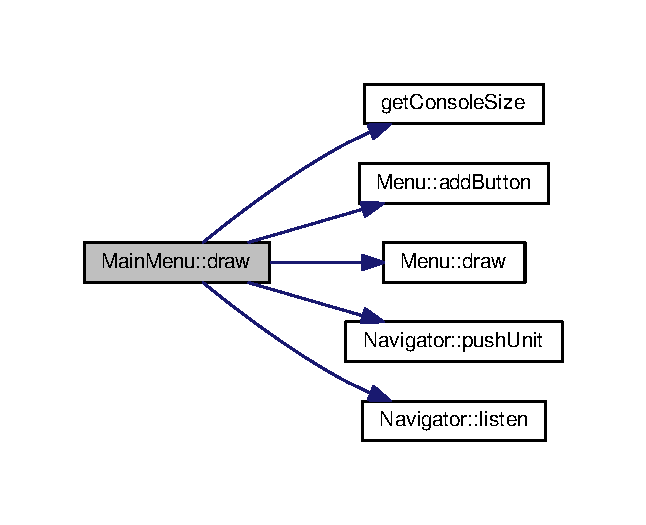
\includegraphics[width=309pt]{class_main_menu_a6c17addf154519404a791d3c2a40a2aa_cgraph}
\end{center}
\end{figure}


The documentation for this class was generated from the following files\+:\begin{DoxyCompactItemize}
\item 
Libraries/\+Screens/\mbox{\hyperlink{main_menu_8h}{main\+Menu.\+h}}\item 
Libraries/\+Screens/\mbox{\hyperlink{main_menu_8cpp}{main\+Menu.\+cpp}}\end{DoxyCompactItemize}

\hypertarget{class_menu}{\section{Menu Class Reference}
\label{class_menu}\index{Menu@{Menu}}
}


{\ttfamily \#include $<$menu.\-h$>$}



Inheritance diagram for Menu\-:
\nopagebreak
\begin{figure}[H]
\begin{center}
\leavevmode
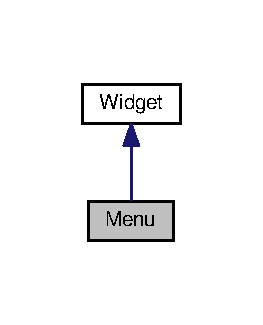
\includegraphics[width=126pt]{class_menu__inherit__graph}
\end{center}
\end{figure}


Collaboration diagram for Menu\-:
\nopagebreak
\begin{figure}[H]
\begin{center}
\leavevmode
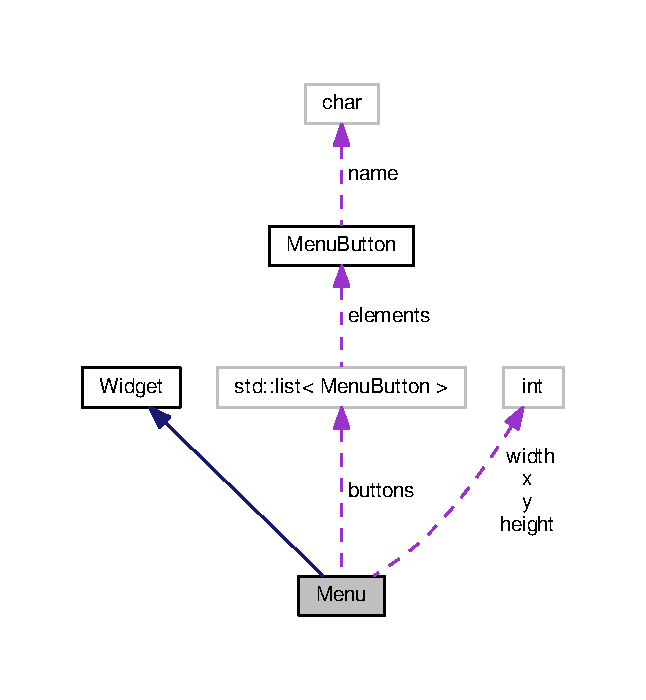
\includegraphics[width=310pt]{class_menu__coll__graph}
\end{center}
\end{figure}
\subsection*{Public Member Functions}
\begin{DoxyCompactItemize}
\item 
void \hyperlink{class_menu_a1a1982871bb5f8b1557d26b0d9ccfe0f}{add\-Button} (const char $\ast$name)
\item 
void \hyperlink{class_menu_ac5ec365a1916cc9cbd233063544588d7}{focus} (int index)
\item 
void \hyperlink{class_menu_acc8b2492f87ebc9219eaad0fe0ecaa5c}{unfocus} (int index)
\item 
void \hyperlink{class_menu_a2cd7ab9901a8f42a3ae977d0774398a6}{draw} ()
\item 
\hyperlink{class_menu_ab6e38ad7f84b7741846cf5a57040276a}{Menu} (int \hyperlink{class_menu_a26c11055ab1fe19a4862689d4ff85dc7}{x}, int \hyperlink{class_menu_a658438f1d47ccb1cfb78b14fe3e09b52}{y}, int \hyperlink{class_menu_a30ec519ffccb75388150c64175c4959b}{width}, int \hyperlink{class_menu_abfd154ce7b19dca62d1ce8483c6f7bba}{height})
\end{DoxyCompactItemize}
\subsection*{Private Attributes}
\begin{DoxyCompactItemize}
\item 
std\-::list$<$ \hyperlink{struct_menu_button}{Menu\-Button} $>$ \hyperlink{class_menu_a631c3c73e1f05159ddc2e967b7b4bca7}{buttons}
\item 
int \hyperlink{class_menu_a26c11055ab1fe19a4862689d4ff85dc7}{x}
\item 
int \hyperlink{class_menu_a658438f1d47ccb1cfb78b14fe3e09b52}{y}
\item 
int \hyperlink{class_menu_a30ec519ffccb75388150c64175c4959b}{width}
\item 
int \hyperlink{class_menu_abfd154ce7b19dca62d1ce8483c6f7bba}{height}
\end{DoxyCompactItemize}


\subsection{Detailed Description}
\hyperlink{class_menu}{Menu} (list of selestable items) widget class 
\begin{DoxyParams}{Parameters}
{\em \{list$<$\-Menu\-Button$>$\}} & buttons -\/ buttons included in menu \\
\hline
{\em \{int\}} & x -\/ x coordinate of left menu side \\
\hline
{\em \{int\}} & y -\/ y coordinate of top menu side \\
\hline
{\em \{int\}} & width -\/ menu width \\
\hline
{\em \{int\}} & height -\/ menu height \\
\hline
\end{DoxyParams}


Definition at line 25 of file menu.\-h.



\subsection{Constructor \& Destructor Documentation}
\hypertarget{class_menu_ab6e38ad7f84b7741846cf5a57040276a}{\index{Menu@{Menu}!Menu@{Menu}}
\index{Menu@{Menu}!Menu@{Menu}}
\subsubsection[{Menu}]{\setlength{\rightskip}{0pt plus 5cm}Menu\-::\-Menu (
\begin{DoxyParamCaption}
\item[{int}]{x, }
\item[{int}]{y, }
\item[{int}]{width, }
\item[{int}]{height}
\end{DoxyParamCaption}
)}}\label{class_menu_ab6e38ad7f84b7741846cf5a57040276a}

\begin{DoxyParams}{Parameters}
{\em \{int\}} & x -\/ x coordinate of left menu side \\
\hline
{\em \{int\}} & y -\/ y coordinate of top menu side \\
\hline
{\em \{int\}} & width -\/ menu width \\
\hline
{\em \{int\}} & height -\/ menu height \\
\hline
\end{DoxyParams}


Definition at line 58 of file menu.\-cpp.



\subsection{Member Function Documentation}
\hypertarget{class_menu_a1a1982871bb5f8b1557d26b0d9ccfe0f}{\index{Menu@{Menu}!add\-Button@{add\-Button}}
\index{add\-Button@{add\-Button}!Menu@{Menu}}
\subsubsection[{add\-Button}]{\setlength{\rightskip}{0pt plus 5cm}void Menu\-::add\-Button (
\begin{DoxyParamCaption}
\item[{const char $\ast$}]{name}
\end{DoxyParamCaption}
)}}\label{class_menu_a1a1982871bb5f8b1557d26b0d9ccfe0f}
Adds button to the menu 
\begin{DoxyParams}{Parameters}
{\em \{const} & char$\ast$\} name -\/ text drawn at the button \\
\hline
\end{DoxyParams}


Definition at line 7 of file menu.\-cpp.



Here is the caller graph for this function\-:
\nopagebreak
\begin{figure}[H]
\begin{center}
\leavevmode
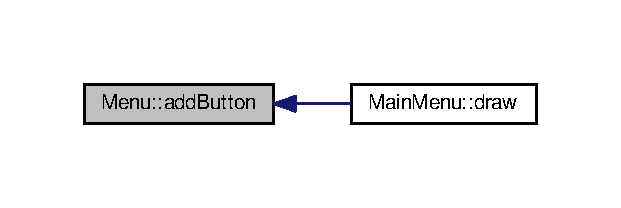
\includegraphics[width=298pt]{class_menu_a1a1982871bb5f8b1557d26b0d9ccfe0f_icgraph}
\end{center}
\end{figure}


\hypertarget{class_menu_a2cd7ab9901a8f42a3ae977d0774398a6}{\index{Menu@{Menu}!draw@{draw}}
\index{draw@{draw}!Menu@{Menu}}
\subsubsection[{draw}]{\setlength{\rightskip}{0pt plus 5cm}void Menu\-::draw (
\begin{DoxyParamCaption}
{}
\end{DoxyParamCaption}
)}}\label{class_menu_a2cd7ab9901a8f42a3ae977d0774398a6}
Draws \hyperlink{class_menu}{Menu} in console window 

Definition at line 39 of file menu.\-cpp.



Here is the caller graph for this function\-:
\nopagebreak
\begin{figure}[H]
\begin{center}
\leavevmode
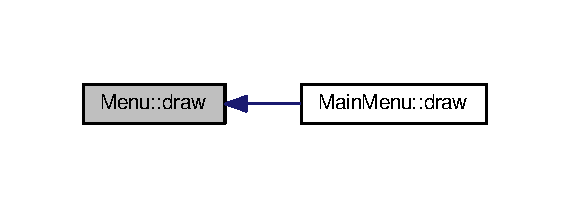
\includegraphics[width=274pt]{class_menu_a2cd7ab9901a8f42a3ae977d0774398a6_icgraph}
\end{center}
\end{figure}


\hypertarget{class_menu_ac5ec365a1916cc9cbd233063544588d7}{\index{Menu@{Menu}!focus@{focus}}
\index{focus@{focus}!Menu@{Menu}}
\subsubsection[{focus}]{\setlength{\rightskip}{0pt plus 5cm}void Menu\-::focus (
\begin{DoxyParamCaption}
\item[{int}]{index}
\end{DoxyParamCaption}
)\hspace{0.3cm}{\ttfamily [virtual]}}}\label{class_menu_ac5ec365a1916cc9cbd233063544588d7}
Event listener activated by \hyperlink{class_navigator}{Navigator} module when user selects on widget   Navigator\-::listener 
\begin{DoxyParams}{Parameters}
{\em \{int\}} & index -\/ index of subunit of the widget \\
\hline
\end{DoxyParams}


Reimplemented from \hyperlink{class_widget_ac395fbcfd90f5a33a4bb2ca1d83631ca}{Widget}.



Definition at line 18 of file menu.\-cpp.

\hypertarget{class_menu_acc8b2492f87ebc9219eaad0fe0ecaa5c}{\index{Menu@{Menu}!unfocus@{unfocus}}
\index{unfocus@{unfocus}!Menu@{Menu}}
\subsubsection[{unfocus}]{\setlength{\rightskip}{0pt plus 5cm}void Menu\-::unfocus (
\begin{DoxyParamCaption}
\item[{int}]{index}
\end{DoxyParamCaption}
)\hspace{0.3cm}{\ttfamily [virtual]}}}\label{class_menu_acc8b2492f87ebc9219eaad0fe0ecaa5c}
Event listener activated by \hyperlink{class_navigator}{Navigator} module when user removes selection from widget   Navigator\-::listener 
\begin{DoxyParams}{Parameters}
{\em \{int\}} & index -\/ index of subunit of the widget \\
\hline
\end{DoxyParams}


Reimplemented from \hyperlink{class_widget_a65f349812facca8302957a83b161a840}{Widget}.



Definition at line 30 of file menu.\-cpp.



\subsection{Member Data Documentation}
\hypertarget{class_menu_a631c3c73e1f05159ddc2e967b7b4bca7}{\index{Menu@{Menu}!buttons@{buttons}}
\index{buttons@{buttons}!Menu@{Menu}}
\subsubsection[{buttons}]{\setlength{\rightskip}{0pt plus 5cm}std\-::list$<${\bf Menu\-Button}$>$ Menu\-::buttons\hspace{0.3cm}{\ttfamily [private]}}}\label{class_menu_a631c3c73e1f05159ddc2e967b7b4bca7}


Definition at line 28 of file menu.\-h.

\hypertarget{class_menu_abfd154ce7b19dca62d1ce8483c6f7bba}{\index{Menu@{Menu}!height@{height}}
\index{height@{height}!Menu@{Menu}}
\subsubsection[{height}]{\setlength{\rightskip}{0pt plus 5cm}int Menu\-::height\hspace{0.3cm}{\ttfamily [private]}}}\label{class_menu_abfd154ce7b19dca62d1ce8483c6f7bba}


Definition at line 29 of file menu.\-h.

\hypertarget{class_menu_a30ec519ffccb75388150c64175c4959b}{\index{Menu@{Menu}!width@{width}}
\index{width@{width}!Menu@{Menu}}
\subsubsection[{width}]{\setlength{\rightskip}{0pt plus 5cm}int Menu\-::width\hspace{0.3cm}{\ttfamily [private]}}}\label{class_menu_a30ec519ffccb75388150c64175c4959b}


Definition at line 29 of file menu.\-h.

\hypertarget{class_menu_a26c11055ab1fe19a4862689d4ff85dc7}{\index{Menu@{Menu}!x@{x}}
\index{x@{x}!Menu@{Menu}}
\subsubsection[{x}]{\setlength{\rightskip}{0pt plus 5cm}int Menu\-::x\hspace{0.3cm}{\ttfamily [private]}}}\label{class_menu_a26c11055ab1fe19a4862689d4ff85dc7}


Definition at line 29 of file menu.\-h.

\hypertarget{class_menu_a658438f1d47ccb1cfb78b14fe3e09b52}{\index{Menu@{Menu}!y@{y}}
\index{y@{y}!Menu@{Menu}}
\subsubsection[{y}]{\setlength{\rightskip}{0pt plus 5cm}int Menu\-::y\hspace{0.3cm}{\ttfamily [private]}}}\label{class_menu_a658438f1d47ccb1cfb78b14fe3e09b52}


Definition at line 29 of file menu.\-h.



The documentation for this class was generated from the following files\-:\begin{DoxyCompactItemize}
\item 
/home/travis/build/echo-\/team/\-Snoke/\-Libraries/\-Interface/\hyperlink{menu_8h}{menu.\-h}\item 
/home/travis/build/echo-\/team/\-Snoke/\-Libraries/\-Interface/\hyperlink{menu_8cpp}{menu.\-cpp}\end{DoxyCompactItemize}

\hypertarget{struct_menu_button}{\section{Menu\-Button Struct Reference}
\label{struct_menu_button}\index{Menu\-Button@{Menu\-Button}}
}


{\ttfamily \#include $<$menu.\-h$>$}



Collaboration diagram for Menu\-Button\-:
\nopagebreak
\begin{figure}[H]
\begin{center}
\leavevmode
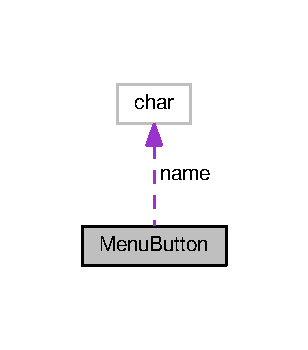
\includegraphics[width=148pt]{struct_menu_button__coll__graph}
\end{center}
\end{figure}
\subsection*{Public Attributes}
\begin{DoxyCompactItemize}
\item 
const char $\ast$ \hyperlink{struct_menu_button_ab20cd84f0366cbb5475c5b1e8de9d72c}{name}
\end{DoxyCompactItemize}


\subsection{Detailed Description}
Describes menu button 
\begin{DoxyParams}{Parameters}
{\em \{const} & char$\ast$\} name -\/ text drawn at the button \\
\hline
\end{DoxyParams}


Definition at line 12 of file menu.\-h.



\subsection{Member Data Documentation}
\hypertarget{struct_menu_button_ab20cd84f0366cbb5475c5b1e8de9d72c}{\index{Menu\-Button@{Menu\-Button}!name@{name}}
\index{name@{name}!MenuButton@{Menu\-Button}}
\subsubsection[{name}]{\setlength{\rightskip}{0pt plus 5cm}const char$\ast$ Menu\-Button\-::name}}\label{struct_menu_button_ab20cd84f0366cbb5475c5b1e8de9d72c}


Definition at line 14 of file menu.\-h.



The documentation for this struct was generated from the following file\-:\begin{DoxyCompactItemize}
\item 
/home/travis/build/echo-\/team/\-Snoke/\-Libraries/\-Interface/\hyperlink{menu_8h}{menu.\-h}\end{DoxyCompactItemize}

\hypertarget{struct_navigate_unit}{}\section{Navigate\+Unit Struct Reference}
\label{struct_navigate_unit}\index{NavigateUnit@{NavigateUnit}}


{\ttfamily \#include $<$navigator.\+h$>$}



Collaboration diagram for Navigate\+Unit\+:
\nopagebreak
\begin{figure}[H]
\begin{center}
\leavevmode
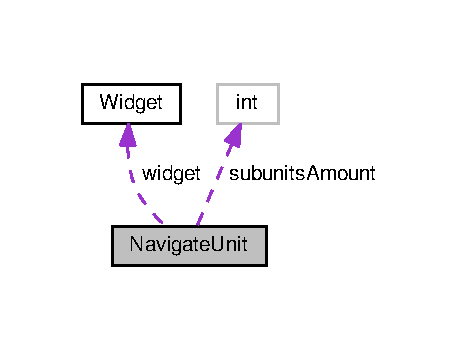
\includegraphics[width=221pt]{struct_navigate_unit__coll__graph}
\end{center}
\end{figure}
\subsection*{Public Attributes}
\begin{DoxyCompactItemize}
\item 
\mbox{\hyperlink{class_widget}{Widget}} $\ast$ \mbox{\hyperlink{struct_navigate_unit_a04a97a78df45d0f2268b8352f64d43f5}{widget}}
\item 
int \mbox{\hyperlink{struct_navigate_unit_a59e42d03540ccad6017bc708cab71893}{subunits\+Amount}}
\end{DoxyCompactItemize}


\subsection{Detailed Description}
Describes selectable/interactive widget or the group of widgets 
\begin{DoxyParams}{Parameters}
{\em \{\+Widget$\ast$\}} & widget -\/ selectable widget class \\
\hline
{\em \{int\}} & subunits\+Amount -\/ amount of user actions to move to another widget (e.\+g\+: amount of subwidgets or lines in the scrollbox) \\
\hline
\end{DoxyParams}


Definition at line 12 of file navigator.\+h.



\subsection{Member Data Documentation}
\mbox{\Hypertarget{struct_navigate_unit_a59e42d03540ccad6017bc708cab71893}\label{struct_navigate_unit_a59e42d03540ccad6017bc708cab71893}} 
\index{NavigateUnit@{NavigateUnit}!subunitsAmount@{subunitsAmount}}
\index{subunitsAmount@{subunitsAmount}!NavigateUnit@{NavigateUnit}}
\subsubsection{\texorpdfstring{subunitsAmount}{subunitsAmount}}
{\footnotesize\ttfamily int Navigate\+Unit\+::subunits\+Amount}



Definition at line 15 of file navigator.\+h.

\mbox{\Hypertarget{struct_navigate_unit_a04a97a78df45d0f2268b8352f64d43f5}\label{struct_navigate_unit_a04a97a78df45d0f2268b8352f64d43f5}} 
\index{NavigateUnit@{NavigateUnit}!widget@{widget}}
\index{widget@{widget}!NavigateUnit@{NavigateUnit}}
\subsubsection{\texorpdfstring{widget}{widget}}
{\footnotesize\ttfamily \mbox{\hyperlink{class_widget}{Widget}}$\ast$ Navigate\+Unit\+::widget}



Definition at line 14 of file navigator.\+h.



The documentation for this struct was generated from the following file\+:\begin{DoxyCompactItemize}
\item 
Libraries/\+Interface/\mbox{\hyperlink{navigator_8h}{navigator.\+h}}\end{DoxyCompactItemize}

\hypertarget{class_navigator}{}\section{Navigator Class Reference}
\label{class_navigator}\index{Navigator@{Navigator}}


{\ttfamily \#include $<$navigator.\+h$>$}



Collaboration diagram for Navigator\+:
\nopagebreak
\begin{figure}[H]
\begin{center}
\leavevmode
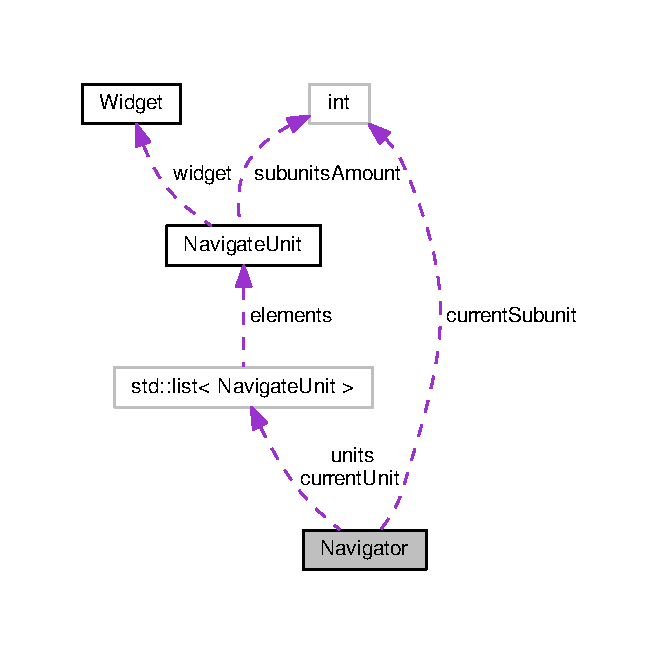
\includegraphics[width=321pt]{class_navigator__coll__graph}
\end{center}
\end{figure}
\subsection*{Public Member Functions}
\begin{DoxyCompactItemize}
\item 
void \mbox{\hyperlink{class_navigator_a47967fc9bdfd276c98f8ed1c44d5dc46}{push\+Unit}} (\mbox{\hyperlink{class_widget}{Widget}} $\ast$unit, int subunits\+Amount)
\item 
void \mbox{\hyperlink{class_navigator_ab9b30029b9ef06cca27ebc5b2549121c}{listen}} ()
\item 
\mbox{\hyperlink{class_navigator_a59230ab4698882f754d5ce275a1a4030}{Navigator}} ()
\end{DoxyCompactItemize}
\subsection*{Private Attributes}
\begin{DoxyCompactItemize}
\item 
std\+::list$<$ \mbox{\hyperlink{struct_navigate_unit}{Navigate\+Unit}} $>$ \mbox{\hyperlink{class_navigator_ad830f88cb2d1b38f7ff49797e244892d}{units}}
\item 
std\+::list$<$ \mbox{\hyperlink{struct_navigate_unit}{Navigate\+Unit}} $>$\+::iterator \mbox{\hyperlink{class_navigator_a64d901b59121319cb87ca450dcc25912}{current\+Unit}}
\item 
int \mbox{\hyperlink{class_navigator_a616e5c7457f641e3027f68103e0da245}{current\+Subunit}}
\end{DoxyCompactItemize}


\subsection{Detailed Description}
Adds an ability to select/activate widgets 
\begin{DoxyParams}{Parameters}
{\em \{list$<$\+Navigate\+Unit$>$\}} & units -\/ widgets/groups of widgets which can be selected \\
\hline
{\em \{list$<$\+Navigate\+Unit$>$\+::iterator\}} & current\+Unit -\/ selected widget \\
\hline
{\em \{int\}} & current\+Subunit -\/ number of subwidget \\
\hline
\end{DoxyParams}


Definition at line 24 of file navigator.\+h.



\subsection{Constructor \& Destructor Documentation}
\mbox{\Hypertarget{class_navigator_a59230ab4698882f754d5ce275a1a4030}\label{class_navigator_a59230ab4698882f754d5ce275a1a4030}} 
\index{Navigator@{Navigator}!Navigator@{Navigator}}
\index{Navigator@{Navigator}!Navigator@{Navigator}}
\subsubsection{\texorpdfstring{Navigator()}{Navigator()}}
{\footnotesize\ttfamily Navigator\+::\+Navigator (\begin{DoxyParamCaption}{ }\end{DoxyParamCaption})}

@constructor 

Definition at line 72 of file navigator.\+cpp.



\subsection{Member Function Documentation}
\mbox{\Hypertarget{class_navigator_ab9b30029b9ef06cca27ebc5b2549121c}\label{class_navigator_ab9b30029b9ef06cca27ebc5b2549121c}} 
\index{Navigator@{Navigator}!listen@{listen}}
\index{listen@{listen}!Navigator@{Navigator}}
\subsubsection{\texorpdfstring{listen()}{listen()}}
{\footnotesize\ttfamily void Navigator\+::listen (\begin{DoxyParamCaption}{ }\end{DoxyParamCaption})}

Starts main loop of application to catch selections and activate events done by user 

Definition at line 16 of file navigator.\+cpp.

Here is the caller graph for this function\+:
\nopagebreak
\begin{figure}[H]
\begin{center}
\leavevmode
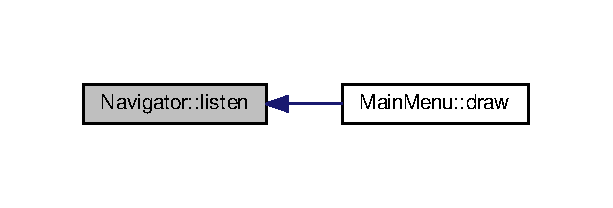
\includegraphics[width=293pt]{class_navigator_ab9b30029b9ef06cca27ebc5b2549121c_icgraph}
\end{center}
\end{figure}
\mbox{\Hypertarget{class_navigator_a47967fc9bdfd276c98f8ed1c44d5dc46}\label{class_navigator_a47967fc9bdfd276c98f8ed1c44d5dc46}} 
\index{Navigator@{Navigator}!pushUnit@{pushUnit}}
\index{pushUnit@{pushUnit}!Navigator@{Navigator}}
\subsubsection{\texorpdfstring{pushUnit()}{pushUnit()}}
{\footnotesize\ttfamily void Navigator\+::push\+Unit (\begin{DoxyParamCaption}\item[{\mbox{\hyperlink{class_widget}{Widget}} $\ast$}]{unit,  }\item[{int}]{subunits\+Amount }\end{DoxyParamCaption})}

Adds selectable widget to the end of selectable widgets queue 
\begin{DoxyParams}{Parameters}
{\em \{\+Widget$\ast$\}} & unit -\/ seleclable widget \\
\hline
{\em \{int} & \} subunits\+Amount -\/ amount of subwidgets \\
\hline
\end{DoxyParams}


Definition at line 8 of file navigator.\+cpp.

Here is the caller graph for this function\+:
\nopagebreak
\begin{figure}[H]
\begin{center}
\leavevmode
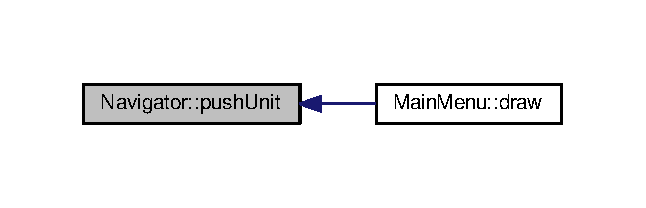
\includegraphics[width=309pt]{class_navigator_a47967fc9bdfd276c98f8ed1c44d5dc46_icgraph}
\end{center}
\end{figure}


\subsection{Member Data Documentation}
\mbox{\Hypertarget{class_navigator_a616e5c7457f641e3027f68103e0da245}\label{class_navigator_a616e5c7457f641e3027f68103e0da245}} 
\index{Navigator@{Navigator}!currentSubunit@{currentSubunit}}
\index{currentSubunit@{currentSubunit}!Navigator@{Navigator}}
\subsubsection{\texorpdfstring{currentSubunit}{currentSubunit}}
{\footnotesize\ttfamily int Navigator\+::current\+Subunit\hspace{0.3cm}{\ttfamily [private]}}



Definition at line 29 of file navigator.\+h.

\mbox{\Hypertarget{class_navigator_a64d901b59121319cb87ca450dcc25912}\label{class_navigator_a64d901b59121319cb87ca450dcc25912}} 
\index{Navigator@{Navigator}!currentUnit@{currentUnit}}
\index{currentUnit@{currentUnit}!Navigator@{Navigator}}
\subsubsection{\texorpdfstring{currentUnit}{currentUnit}}
{\footnotesize\ttfamily std\+::list$<$\mbox{\hyperlink{struct_navigate_unit}{Navigate\+Unit}}$>$\+::iterator Navigator\+::current\+Unit\hspace{0.3cm}{\ttfamily [private]}}



Definition at line 28 of file navigator.\+h.

\mbox{\Hypertarget{class_navigator_ad830f88cb2d1b38f7ff49797e244892d}\label{class_navigator_ad830f88cb2d1b38f7ff49797e244892d}} 
\index{Navigator@{Navigator}!units@{units}}
\index{units@{units}!Navigator@{Navigator}}
\subsubsection{\texorpdfstring{units}{units}}
{\footnotesize\ttfamily std\+::list$<$\mbox{\hyperlink{struct_navigate_unit}{Navigate\+Unit}}$>$ Navigator\+::units\hspace{0.3cm}{\ttfamily [private]}}



Definition at line 27 of file navigator.\+h.



The documentation for this class was generated from the following files\+:\begin{DoxyCompactItemize}
\item 
Libraries/\+Interface/\mbox{\hyperlink{navigator_8h}{navigator.\+h}}\item 
Libraries/\+Interface/\mbox{\hyperlink{navigator_8cpp}{navigator.\+cpp}}\end{DoxyCompactItemize}

\hypertarget{struct_side_button}{}\section{Side\+Button Struct Reference}
\label{struct_side_button}\index{SideButton@{SideButton}}


{\ttfamily \#include $<$Side\+Menu.\+h$>$}



Collaboration diagram for Side\+Button\+:
\nopagebreak
\begin{figure}[H]
\begin{center}
\leavevmode
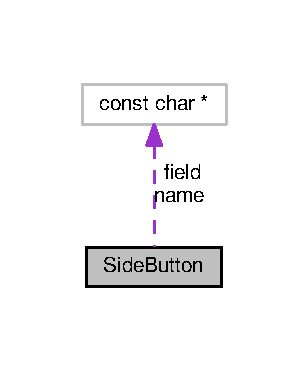
\includegraphics[width=149pt]{struct_side_button__coll__graph}
\end{center}
\end{figure}
\subsection*{Public Attributes}
\begin{DoxyCompactItemize}
\item 
const char $\ast$ \mbox{\hyperlink{struct_side_button_a2533e6acfd5ba40cb7717412c25e6a0c}{name}}
\item 
const char $\ast$ \mbox{\hyperlink{struct_side_button_afd703657d0b75b20a7ca1d2c3147ec34}{field}}
\end{DoxyCompactItemize}


\subsection{Detailed Description}


Definition at line 4 of file Side\+Menu.\+h.



\subsection{Member Data Documentation}
\mbox{\Hypertarget{struct_side_button_afd703657d0b75b20a7ca1d2c3147ec34}\label{struct_side_button_afd703657d0b75b20a7ca1d2c3147ec34}} 
\index{SideButton@{SideButton}!field@{field}}
\index{field@{field}!SideButton@{SideButton}}
\subsubsection{\texorpdfstring{field}{field}}
{\footnotesize\ttfamily const char$\ast$ Side\+Button\+::field}



Definition at line 7 of file Side\+Menu.\+h.

\mbox{\Hypertarget{struct_side_button_a2533e6acfd5ba40cb7717412c25e6a0c}\label{struct_side_button_a2533e6acfd5ba40cb7717412c25e6a0c}} 
\index{SideButton@{SideButton}!name@{name}}
\index{name@{name}!SideButton@{SideButton}}
\subsubsection{\texorpdfstring{name}{name}}
{\footnotesize\ttfamily const char$\ast$ Side\+Button\+::name}



Definition at line 6 of file Side\+Menu.\+h.



The documentation for this struct was generated from the following file\+:\begin{DoxyCompactItemize}
\item 
Libraries/\+Side\+Menu/\mbox{\hyperlink{_side_menu_8h}{Side\+Menu.\+h}}\end{DoxyCompactItemize}

\hypertarget{class_side_menu}{}\section{Side\+Menu Class Reference}
\label{class_side_menu}\index{SideMenu@{SideMenu}}


{\ttfamily \#include $<$Side\+Menu.\+h$>$}



Collaboration diagram for Side\+Menu\+:
\nopagebreak
\begin{figure}[H]
\begin{center}
\leavevmode
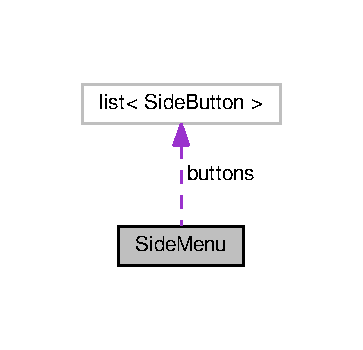
\includegraphics[width=175pt]{class_side_menu__coll__graph}
\end{center}
\end{figure}
\subsection*{Private Attributes}
\begin{DoxyCompactItemize}
\item 
list$<$ \mbox{\hyperlink{struct_side_button}{Side\+Button}} $>$ \mbox{\hyperlink{class_side_menu_af6b73f113ae5b74a238f5b167c8902cb}{buttons}}
\end{DoxyCompactItemize}


\subsection{Detailed Description}


Definition at line 11 of file Side\+Menu.\+h.



\subsection{Member Data Documentation}
\mbox{\Hypertarget{class_side_menu_af6b73f113ae5b74a238f5b167c8902cb}\label{class_side_menu_af6b73f113ae5b74a238f5b167c8902cb}} 
\index{SideMenu@{SideMenu}!buttons@{buttons}}
\index{buttons@{buttons}!SideMenu@{SideMenu}}
\subsubsection{\texorpdfstring{buttons}{buttons}}
{\footnotesize\ttfamily list$<$\mbox{\hyperlink{struct_side_button}{Side\+Button}}$>$ Side\+Menu\+::buttons\hspace{0.3cm}{\ttfamily [private]}}



Definition at line 14 of file Side\+Menu.\+h.



The documentation for this class was generated from the following file\+:\begin{DoxyCompactItemize}
\item 
Libraries/\+Side\+Menu/\mbox{\hyperlink{_side_menu_8h}{Side\+Menu.\+h}}\end{DoxyCompactItemize}

\hypertarget{class_snake}{}\section{Snake Class Reference}
\label{class_snake}\index{Snake@{Snake}}


{\ttfamily \#include $<$snake.\+h$>$}



Collaboration diagram for Snake\+:
\nopagebreak
\begin{figure}[H]
\begin{center}
\leavevmode
\includegraphics[width=313pt]{class_snake__coll__graph}
\end{center}
\end{figure}
\subsection*{Public Member Functions}
\begin{DoxyCompactItemize}
\item 
bool \mbox{\hyperlink{class_snake_a953fb7b8be521f651989bb53323e89ec}{init}} (\mbox{\hyperlink{common_8h_aa9cfdb80b4ca12013a2de8a3b9b97981}{Point}} begin, short \mbox{\hyperlink{class_snake_aee6d8cb1404c33a9b7e132a99e055590}{direction}}, int length)
\item 
void \mbox{\hyperlink{class_snake_a0c305e807c15736f809eb035d947c988}{set\+Scheme}} ()
\item 
void \mbox{\hyperlink{class_snake_a62fa59de03f60c23f6d1100c53594d71}{get\+Coords}} (std\+::list$<$ \mbox{\hyperlink{common_8h_aa9cfdb80b4ca12013a2de8a3b9b97981}{Point}} $>$ $\ast$curr\+Body)
\item 
\mbox{\hyperlink{common_8h_aa9cfdb80b4ca12013a2de8a3b9b97981}{Point}} \mbox{\hyperlink{class_snake_a0235581bc3d6399f4fd2287669f93cee}{get\+Head\+Coords}} ()
\item 
void \mbox{\hyperlink{class_snake_a151d9cab8233d38524c09642d079356a}{set\+Direction}} (int dir=0)
\item 
short \mbox{\hyperlink{class_snake_a2656a9a4490cbb70d305c323269cc5bd}{get\+Direction}} ()
\item 
bool \mbox{\hyperlink{class_snake_a6181d41b0920aff3fda1a90d59e8d382}{move}} (\mbox{\hyperlink{class_labyrinth}{Labyrinth}} labyrinth, \mbox{\hyperlink{class_ball}{Ball}} $\ast$ball, \mbox{\hyperlink{common_8h_aa9cfdb80b4ca12013a2de8a3b9b97981}{Point}} $\ast$change\mbox{[}2\mbox{]}, int change\+Size)
\end{DoxyCompactItemize}
\subsection*{Private Member Functions}
\begin{DoxyCompactItemize}
\item 
short \mbox{\hyperlink{class_snake_a7df802733cb62081ea360bb81ba9f304}{check\+Intersection}} (\mbox{\hyperlink{common_8h_aa9cfdb80b4ca12013a2de8a3b9b97981}{Point}} check, \mbox{\hyperlink{class_labyrinth}{Labyrinth}} laryrinth, \mbox{\hyperlink{class_ball}{Ball}} $\ast$ball)
\item 
short \mbox{\hyperlink{class_snake_a2f8cc670284cdebf4c9bbe60a7296deb}{check\+Wisely}} (\mbox{\hyperlink{common_8h_aa9cfdb80b4ca12013a2de8a3b9b97981}{Point}} coords, \mbox{\hyperlink{common_8h_aa9cfdb80b4ca12013a2de8a3b9b97981}{Point}} bcoords)
\item 
void \mbox{\hyperlink{class_snake_a59b2f5b18ab563d1583dfb15064784a0}{move\+Head}} (\mbox{\hyperlink{common_8h_aa9cfdb80b4ca12013a2de8a3b9b97981}{Point}} p, \mbox{\hyperlink{common_8h_aa9cfdb80b4ca12013a2de8a3b9b97981}{Point}} $\ast$change\mbox{[}2\mbox{]})
\item 
void \mbox{\hyperlink{class_snake_a577892c68b457316f7a9f3944c464569}{move\+Back}} (\mbox{\hyperlink{common_8h_aa9cfdb80b4ca12013a2de8a3b9b97981}{Point}} p, \mbox{\hyperlink{common_8h_aa9cfdb80b4ca12013a2de8a3b9b97981}{Point}} $\ast$cahnge\mbox{[}2\mbox{]})
\end{DoxyCompactItemize}
\subsection*{Private Attributes}
\begin{DoxyCompactItemize}
\item 
short \mbox{\hyperlink{class_snake_aee6d8cb1404c33a9b7e132a99e055590}{direction}}
\item 
std\+::list$<$ \mbox{\hyperlink{common_8h_afd9cb36d6ef309c77ea1e3177e19c623}{Point\+Style}} $>$ \mbox{\hyperlink{class_snake_a7db439ed2dd1cfea4c061e6ffd6ec54c}{style}}
\item 
std\+::deque$<$ \mbox{\hyperlink{common_8h_aa9cfdb80b4ca12013a2de8a3b9b97981}{Point}} $>$ \mbox{\hyperlink{class_snake_aaf288745dcc19ef13a1330bb55f1471c}{snake\+Body}}
\end{DoxyCompactItemize}


\subsection{Detailed Description}
Describes the snake entity of the game 
\begin{DoxyParams}{Parameters}
{\em \{short\}} & direction -\/ current direction where the snake is heading; \\
\hline
{\em \{list$<$\+Point\+Style$>$\}} & style -\/ an array, describing how should the snake be colored \\
\hline
{\em \{deque$<$\+Point$>$\}} & snake\+Body -\/ a deque type array, containing sposition of snake\textquotesingle{}s body segments \\
\hline
\end{DoxyParams}


Definition at line 50 of file snake.\+h.



\subsection{Member Function Documentation}
\mbox{\Hypertarget{class_snake_a7df802733cb62081ea360bb81ba9f304}\label{class_snake_a7df802733cb62081ea360bb81ba9f304}} 
\index{Snake@{Snake}!checkIntersection@{checkIntersection}}
\index{checkIntersection@{checkIntersection}!Snake@{Snake}}
\subsubsection{\texorpdfstring{checkIntersection()}{checkIntersection()}}
{\footnotesize\ttfamily short Snake\+::check\+Intersection (\begin{DoxyParamCaption}\item[{\mbox{\hyperlink{common_8h_aa9cfdb80b4ca12013a2de8a3b9b97981}{Point}}}]{check,  }\item[{\mbox{\hyperlink{class_labyrinth}{Labyrinth}}}]{labyrinth,  }\item[{\mbox{\hyperlink{class_ball}{Ball}} $\ast$}]{ball }\end{DoxyParamCaption})\hspace{0.3cm}{\ttfamily [private]}}

Checking the given point for intersections with \mbox{\hyperlink{class_ball}{Ball}}, borders, obstacles 
\begin{DoxyParams}{Parameters}
{\em \{\+Labyrinth\}} & labyrinth -\/ 2-\/dimensional array defying current state of every point of the game field (blocked or not) \\
\hline
{\em \{\+Ball$\ast$\}} & ball -\/ a pointer to a \mbox{\hyperlink{class_ball}{Ball}} object(to check intersection with) \\
\hline
{\em \{\+Point$\ast$\}} & change -\/ 2-\/dimensional array of changes needed to be applied to the labyrinth \\
\hline
\end{DoxyParams}
\begin{DoxyReturn}{Returns}
\{short\} -\/ type of collision 
\end{DoxyReturn}


Definition at line 191 of file snake.\+cpp.

Here is the call graph for this function\+:
\nopagebreak
\begin{figure}[H]
\begin{center}
\leavevmode
\includegraphics[width=350pt]{class_snake_a7df802733cb62081ea360bb81ba9f304_cgraph}
\end{center}
\end{figure}
Here is the caller graph for this function\+:
\nopagebreak
\begin{figure}[H]
\begin{center}
\leavevmode
\includegraphics[width=350pt]{class_snake_a7df802733cb62081ea360bb81ba9f304_icgraph}
\end{center}
\end{figure}
\mbox{\Hypertarget{class_snake_a2f8cc670284cdebf4c9bbe60a7296deb}\label{class_snake_a2f8cc670284cdebf4c9bbe60a7296deb}} 
\index{Snake@{Snake}!checkWisely@{checkWisely}}
\index{checkWisely@{checkWisely}!Snake@{Snake}}
\subsubsection{\texorpdfstring{checkWisely()}{checkWisely()}}
{\footnotesize\ttfamily short Snake\+::check\+Wisely (\begin{DoxyParamCaption}\item[{\mbox{\hyperlink{common_8h_aa9cfdb80b4ca12013a2de8a3b9b97981}{Point}}}]{coords,  }\item[{\mbox{\hyperlink{common_8h_aa9cfdb80b4ca12013a2de8a3b9b97981}{Point}}}]{bcoords }\end{DoxyParamCaption})\hspace{0.3cm}{\ttfamily [private]}}

If the Point of the labyrinth we are checking is not free then decide the type of collision 
\begin{DoxyParams}{Parameters}
{\em \{\+Point\}} & coords -\/ Point we are checking for type of a collision \\
\hline
{\em \{\+Point\}} & bcoords -\/ Point, containing the coordinates of the \mbox{\hyperlink{class_ball}{Ball}} \\
\hline
\end{DoxyParams}
\begin{DoxyReturn}{Returns}
\{short\} -\/ type of the collision 
\end{DoxyReturn}


Definition at line 207 of file snake.\+cpp.

Here is the caller graph for this function\+:
\nopagebreak
\begin{figure}[H]
\begin{center}
\leavevmode
\includegraphics[width=350pt]{class_snake_a2f8cc670284cdebf4c9bbe60a7296deb_icgraph}
\end{center}
\end{figure}
\mbox{\Hypertarget{class_snake_a62fa59de03f60c23f6d1100c53594d71}\label{class_snake_a62fa59de03f60c23f6d1100c53594d71}} 
\index{Snake@{Snake}!getCoords@{getCoords}}
\index{getCoords@{getCoords}!Snake@{Snake}}
\subsubsection{\texorpdfstring{getCoords()}{getCoords()}}
{\footnotesize\ttfamily void Snake\+::get\+Coords (\begin{DoxyParamCaption}\item[{std\+::list$<$ \mbox{\hyperlink{common_8h_aa9cfdb80b4ca12013a2de8a3b9b97981}{Point}} $>$ $\ast$}]{curr\+Body }\end{DoxyParamCaption})}

The method to get the snake whole body coordinates(x ,y) without giving the direct access 
\begin{DoxyParams}{Parameters}
{\em \{std\+::list$<$\+Point$>$\}} & curr\+Body -\/ an array where the current snake body is copied \\
\hline
\end{DoxyParams}


Definition at line 276 of file snake.\+cpp.

Here is the caller graph for this function\+:
\nopagebreak
\begin{figure}[H]
\begin{center}
\leavevmode
\includegraphics[width=350pt]{class_snake_a62fa59de03f60c23f6d1100c53594d71_icgraph}
\end{center}
\end{figure}
\mbox{\Hypertarget{class_snake_a2656a9a4490cbb70d305c323269cc5bd}\label{class_snake_a2656a9a4490cbb70d305c323269cc5bd}} 
\index{Snake@{Snake}!getDirection@{getDirection}}
\index{getDirection@{getDirection}!Snake@{Snake}}
\subsubsection{\texorpdfstring{getDirection()}{getDirection()}}
{\footnotesize\ttfamily short Snake\+::get\+Direction (\begin{DoxyParamCaption}{ }\end{DoxyParamCaption})}

The method to get the current direction without giving the direct access \begin{DoxyReturn}{Returns}
\{short\} 
\end{DoxyReturn}


Definition at line 255 of file snake.\+cpp.

\mbox{\Hypertarget{class_snake_a0235581bc3d6399f4fd2287669f93cee}\label{class_snake_a0235581bc3d6399f4fd2287669f93cee}} 
\index{Snake@{Snake}!getHeadCoords@{getHeadCoords}}
\index{getHeadCoords@{getHeadCoords}!Snake@{Snake}}
\subsubsection{\texorpdfstring{getHeadCoords()}{getHeadCoords()}}
{\footnotesize\ttfamily \mbox{\hyperlink{common_8h_aa9cfdb80b4ca12013a2de8a3b9b97981}{Point}} Snake\+::get\+Head\+Coords (\begin{DoxyParamCaption}{ }\end{DoxyParamCaption})}

The method to get the coordinates(x, y) of the snake\textquotesingle{}s head without giving the direct access \begin{DoxyReturn}{Returns}
\{Point\} 
\end{DoxyReturn}


Definition at line 264 of file snake.\+cpp.

Here is the caller graph for this function\+:
\nopagebreak
\begin{figure}[H]
\begin{center}
\leavevmode
\includegraphics[width=350pt]{class_snake_a0235581bc3d6399f4fd2287669f93cee_icgraph}
\end{center}
\end{figure}
\mbox{\Hypertarget{class_snake_a953fb7b8be521f651989bb53323e89ec}\label{class_snake_a953fb7b8be521f651989bb53323e89ec}} 
\index{Snake@{Snake}!init@{init}}
\index{init@{init}!Snake@{Snake}}
\subsubsection{\texorpdfstring{init()}{init()}}
{\footnotesize\ttfamily bool Snake\+::init (\begin{DoxyParamCaption}\item[{\mbox{\hyperlink{common_8h_aa9cfdb80b4ca12013a2de8a3b9b97981}{Point}}}]{begin,  }\item[{short}]{dir,  }\item[{int}]{length }\end{DoxyParamCaption})}

Initializes snake 
\begin{DoxyParams}{Parameters}
{\em \{\+Point\}} & begin -\/ starting Point of a snake(where the tail segment will be situated) \\
\hline
{\em \{short\}} & dir -\/ direction of snake\textquotesingle{}s \textquotesingle{}growth\textquotesingle{} as well as it\textquotesingle{}s starting direction \\
\hline
{\em \{int\}} & length -\/ the length of a \textquotesingle{}new born\textquotesingle{} snake \\
\hline
\end{DoxyParams}
\begin{DoxyReturn}{Returns}
\{bool\} -\/ mark of whether the snake is successfully initialized 
\end{DoxyReturn}


Definition at line 10 of file snake.\+cpp.

Here is the caller graph for this function\+:
\nopagebreak
\begin{figure}[H]
\begin{center}
\leavevmode
\includegraphics[width=350pt]{class_snake_a953fb7b8be521f651989bb53323e89ec_icgraph}
\end{center}
\end{figure}
\mbox{\Hypertarget{class_snake_a6181d41b0920aff3fda1a90d59e8d382}\label{class_snake_a6181d41b0920aff3fda1a90d59e8d382}} 
\index{Snake@{Snake}!move@{move}}
\index{move@{move}!Snake@{Snake}}
\subsubsection{\texorpdfstring{move()}{move()}}
{\footnotesize\ttfamily bool Snake\+::move (\begin{DoxyParamCaption}\item[{\mbox{\hyperlink{class_labyrinth}{Labyrinth}}}]{labyrinth,  }\item[{\mbox{\hyperlink{class_ball}{Ball}} $\ast$}]{ball,  }\item[{\mbox{\hyperlink{common_8h_aa9cfdb80b4ca12013a2de8a3b9b97981}{Point}} $\ast$}]{change\mbox{[}2\mbox{]},  }\item[{int}]{change\+Size }\end{DoxyParamCaption})}

The snake movement on the game field(should be called in each iteration of the game cycle, unless the snake is \textquotesingle{}dead\textquotesingle{}) 
\begin{DoxyParams}{Parameters}
{\em \{\+Labyrinth\}} & labyrinth -\/ the current state of the labyrinth object for intersection checking \\
\hline
{\em \{\+Ball$\ast$\}} & ball -\/ a pointer to a \mbox{\hyperlink{class_ball}{Ball}} object(to check intersection with) \\
\hline
{\em \{\+Point$\ast$\}} & change -\/ 2-\/dimensional array of changes needed to be applied to the labyrinth \\
\hline
\end{DoxyParams}
\begin{DoxyReturn}{Returns}
\{bool\} -\/ mark of whether there was a non-\/boundary non-\/ball collision 
\end{DoxyReturn}


Definition at line 61 of file snake.\+cpp.

Here is the call graph for this function\+:
\nopagebreak
\begin{figure}[H]
\begin{center}
\leavevmode
\includegraphics[width=350pt]{class_snake_a6181d41b0920aff3fda1a90d59e8d382_cgraph}
\end{center}
\end{figure}
Here is the caller graph for this function\+:
\nopagebreak
\begin{figure}[H]
\begin{center}
\leavevmode
\includegraphics[width=326pt]{class_snake_a6181d41b0920aff3fda1a90d59e8d382_icgraph}
\end{center}
\end{figure}
\mbox{\Hypertarget{class_snake_a577892c68b457316f7a9f3944c464569}\label{class_snake_a577892c68b457316f7a9f3944c464569}} 
\index{Snake@{Snake}!moveBack@{moveBack}}
\index{moveBack@{moveBack}!Snake@{Snake}}
\subsubsection{\texorpdfstring{moveBack()}{moveBack()}}
{\footnotesize\ttfamily void Snake\+::move\+Back (\begin{DoxyParamCaption}\item[{\mbox{\hyperlink{common_8h_aa9cfdb80b4ca12013a2de8a3b9b97981}{Point}}}]{p,  }\item[{\mbox{\hyperlink{common_8h_aa9cfdb80b4ca12013a2de8a3b9b97981}{Point}} $\ast$}]{change\mbox{[}2\mbox{]} }\end{DoxyParamCaption})\hspace{0.3cm}{\ttfamily [private]}}

Checking if we need to remove the back of the snake from the labyrinth(we don\textquotesingle{}t in case it has eaten the \mbox{\hyperlink{class_ball}{Ball}}) 
\begin{DoxyParams}{Parameters}
{\em \{\+Point\}} & p -\/ the desired position of movement \\
\hline
{\em \{\+Point$\ast$\}} & change -\/ 2-\/dimensional array of changes needed to be applied to the labyrinth \\
\hline
\end{DoxyParams}


Definition at line 175 of file snake.\+cpp.

Here is the caller graph for this function\+:
\nopagebreak
\begin{figure}[H]
\begin{center}
\leavevmode
\includegraphics[width=350pt]{class_snake_a577892c68b457316f7a9f3944c464569_icgraph}
\end{center}
\end{figure}
\mbox{\Hypertarget{class_snake_a59b2f5b18ab563d1583dfb15064784a0}\label{class_snake_a59b2f5b18ab563d1583dfb15064784a0}} 
\index{Snake@{Snake}!moveHead@{moveHead}}
\index{moveHead@{moveHead}!Snake@{Snake}}
\subsubsection{\texorpdfstring{moveHead()}{moveHead()}}
{\footnotesize\ttfamily void Snake\+::move\+Head (\begin{DoxyParamCaption}\item[{\mbox{\hyperlink{common_8h_aa9cfdb80b4ca12013a2de8a3b9b97981}{Point}}}]{p,  }\item[{\mbox{\hyperlink{common_8h_aa9cfdb80b4ca12013a2de8a3b9b97981}{Point}} $\ast$}]{change\mbox{[}2\mbox{]} }\end{DoxyParamCaption})\hspace{0.3cm}{\ttfamily [private]}}

Moving snake head to a described by parameters position and updating the addition to the labyrinth 
\begin{DoxyParams}{Parameters}
{\em \{\+Point\}} & p -\/ the new head position \\
\hline
{\em \{\+Point$\ast$\}} & change -\/ 2-\/dimensional array of changes needed to be applied to the labyrinth \\
\hline
\end{DoxyParams}


Definition at line 164 of file snake.\+cpp.

Here is the caller graph for this function\+:
\nopagebreak
\begin{figure}[H]
\begin{center}
\leavevmode
\includegraphics[width=350pt]{class_snake_a59b2f5b18ab563d1583dfb15064784a0_icgraph}
\end{center}
\end{figure}
\mbox{\Hypertarget{class_snake_a151d9cab8233d38524c09642d079356a}\label{class_snake_a151d9cab8233d38524c09642d079356a}} 
\index{Snake@{Snake}!setDirection@{setDirection}}
\index{setDirection@{setDirection}!Snake@{Snake}}
\subsubsection{\texorpdfstring{setDirection()}{setDirection()}}
{\footnotesize\ttfamily void Snake\+::set\+Direction (\begin{DoxyParamCaption}\item[{int}]{direction = {\ttfamily 0} }\end{DoxyParamCaption})}

The method to set the direction where the snake is heading 
\begin{DoxyParams}{Parameters}
{\em \{int\}} & direction -\/ direction of the snake we are trying to set \\
\hline
\end{DoxyParams}


Definition at line 236 of file snake.\+cpp.

Here is the caller graph for this function\+:
\nopagebreak
\begin{figure}[H]
\begin{center}
\leavevmode
\includegraphics[width=350pt]{class_snake_a151d9cab8233d38524c09642d079356a_icgraph}
\end{center}
\end{figure}
\mbox{\Hypertarget{class_snake_a0c305e807c15736f809eb035d947c988}\label{class_snake_a0c305e807c15736f809eb035d947c988}} 
\index{Snake@{Snake}!setScheme@{setScheme}}
\index{setScheme@{setScheme}!Snake@{Snake}}
\subsubsection{\texorpdfstring{setScheme()}{setScheme()}}
{\footnotesize\ttfamily void Snake\+::set\+Scheme (\begin{DoxyParamCaption}{ }\end{DoxyParamCaption})}



\subsection{Member Data Documentation}
\mbox{\Hypertarget{class_snake_aee6d8cb1404c33a9b7e132a99e055590}\label{class_snake_aee6d8cb1404c33a9b7e132a99e055590}} 
\index{Snake@{Snake}!direction@{direction}}
\index{direction@{direction}!Snake@{Snake}}
\subsubsection{\texorpdfstring{direction}{direction}}
{\footnotesize\ttfamily short Snake\+::direction\hspace{0.3cm}{\ttfamily [private]}}



Definition at line 53 of file snake.\+h.

\mbox{\Hypertarget{class_snake_aaf288745dcc19ef13a1330bb55f1471c}\label{class_snake_aaf288745dcc19ef13a1330bb55f1471c}} 
\index{Snake@{Snake}!snakeBody@{snakeBody}}
\index{snakeBody@{snakeBody}!Snake@{Snake}}
\subsubsection{\texorpdfstring{snakeBody}{snakeBody}}
{\footnotesize\ttfamily std\+::deque$<$\mbox{\hyperlink{common_8h_aa9cfdb80b4ca12013a2de8a3b9b97981}{Point}}$>$ Snake\+::snake\+Body\hspace{0.3cm}{\ttfamily [private]}}



Definition at line 55 of file snake.\+h.

\mbox{\Hypertarget{class_snake_a7db439ed2dd1cfea4c061e6ffd6ec54c}\label{class_snake_a7db439ed2dd1cfea4c061e6ffd6ec54c}} 
\index{Snake@{Snake}!style@{style}}
\index{style@{style}!Snake@{Snake}}
\subsubsection{\texorpdfstring{style}{style}}
{\footnotesize\ttfamily std\+::list$<$\mbox{\hyperlink{common_8h_afd9cb36d6ef309c77ea1e3177e19c623}{Point\+Style}}$>$ Snake\+::style\hspace{0.3cm}{\ttfamily [private]}}



Definition at line 54 of file snake.\+h.



The documentation for this class was generated from the following files\+:\begin{DoxyCompactItemize}
\item 
Libraries/\+Snake/\mbox{\hyperlink{snake_8h}{snake.\+h}}\item 
Libraries/\+Snake/\mbox{\hyperlink{snake_8cpp}{snake.\+cpp}}\end{DoxyCompactItemize}

\hypertarget{class_widget}{}\section{Widget Class Reference}
\label{class_widget}\index{Widget@{Widget}}


{\ttfamily \#include $<$interface.\+h$>$}



Inheritance diagram for Widget\+:
\nopagebreak
\begin{figure}[H]
\begin{center}
\leavevmode
\includegraphics[width=127pt]{class_widget__inherit__graph}
\end{center}
\end{figure}
\subsection*{Public Member Functions}
\begin{DoxyCompactItemize}
\item 
virtual void \mbox{\hyperlink{class_widget_ac395fbcfd90f5a33a4bb2ca1d83631ca}{focus}} (int index)
\item 
virtual void \mbox{\hyperlink{class_widget_a65f349812facca8302957a83b161a840}{unfocus}} (int index)
\end{DoxyCompactItemize}


\subsection{Detailed Description}
Basic class of the console widget (to store different widgets in one list) 

Definition at line 7 of file interface.\+h.



\subsection{Member Function Documentation}
\mbox{\Hypertarget{class_widget_ac395fbcfd90f5a33a4bb2ca1d83631ca}\label{class_widget_ac395fbcfd90f5a33a4bb2ca1d83631ca}} 
\index{Widget@{Widget}!focus@{focus}}
\index{focus@{focus}!Widget@{Widget}}
\subsubsection{\texorpdfstring{focus()}{focus()}}
{\footnotesize\ttfamily void Widget\+::focus (\begin{DoxyParamCaption}\item[{int}]{index }\end{DoxyParamCaption})\hspace{0.3cm}{\ttfamily [virtual]}}

Event listener activated by \mbox{\hyperlink{class_navigator}{Navigator}} module when user selects widget @virtual @callback Navigator\+::listener 
\begin{DoxyParams}{Parameters}
{\em \{int\}} & index -\/ index of subunit of the widget \\
\hline
\end{DoxyParams}


Reimplemented in \mbox{\hyperlink{class_menu_ac5ec365a1916cc9cbd233063544588d7}{Menu}}.



Definition at line 9 of file interface.\+cpp.

\mbox{\Hypertarget{class_widget_a65f349812facca8302957a83b161a840}\label{class_widget_a65f349812facca8302957a83b161a840}} 
\index{Widget@{Widget}!unfocus@{unfocus}}
\index{unfocus@{unfocus}!Widget@{Widget}}
\subsubsection{\texorpdfstring{unfocus()}{unfocus()}}
{\footnotesize\ttfamily void Widget\+::unfocus (\begin{DoxyParamCaption}\item[{int}]{index }\end{DoxyParamCaption})\hspace{0.3cm}{\ttfamily [virtual]}}

Event listener activated by \mbox{\hyperlink{class_navigator}{Navigator}} module when user clicks on widget @virtual @callback Navigator\+::listener 
\begin{DoxyParams}{Parameters}
{\em \{int\}} & index -\/ index of subunit of the widget \\
\hline
\end{DoxyParams}


Reimplemented in \mbox{\hyperlink{class_menu_acc8b2492f87ebc9219eaad0fe0ecaa5c}{Menu}}.



Definition at line 18 of file interface.\+cpp.



The documentation for this class was generated from the following files\+:\begin{DoxyCompactItemize}
\item 
Libraries/\+Interface/\mbox{\hyperlink{interface_8h}{interface.\+h}}\item 
Libraries/\+Interface/\mbox{\hyperlink{interface_8cpp}{interface.\+cpp}}\end{DoxyCompactItemize}

\chapter{File Documentation}
\hypertarget{ball_8cpp}{\section{/home/travis/build/echo-\/team/\-Snoke/\-Libraries/\-Ball/ball.cpp File Reference}
\label{ball_8cpp}\index{/home/travis/build/echo-\/team/\-Snoke/\-Libraries/\-Ball/ball.\-cpp@{/home/travis/build/echo-\/team/\-Snoke/\-Libraries/\-Ball/ball.\-cpp}}
}
{\ttfamily \#include \char`\"{}ball.\-h\char`\"{}}\\*
Include dependency graph for ball.\-cpp\-:
\nopagebreak
\begin{figure}[H]
\begin{center}
\leavevmode
\includegraphics[width=350pt]{ball_8cpp__incl}
\end{center}
\end{figure}

\hypertarget{ball_8h}{}\section{Libraries/\+Ball/ball.h File Reference}
\label{ball_8h}\index{Libraries/Ball/ball.h@{Libraries/Ball/ball.h}}
{\ttfamily \#include \char`\"{}../\+Common/common.\+h\char`\"{}}\newline
{\ttfamily \#include \char`\"{}../\+Labyrinth/labyrinth.\+h\char`\"{}}\newline
{\ttfamily \#include $<$random$>$}\newline
{\ttfamily \#include $<$ctime$>$}\newline
Include dependency graph for ball.\+h\+:
\nopagebreak
\begin{figure}[H]
\begin{center}
\leavevmode
\includegraphics[width=350pt]{ball_8h__incl}
\end{center}
\end{figure}
This graph shows which files directly or indirectly include this file\+:
\nopagebreak
\begin{figure}[H]
\begin{center}
\leavevmode
\includegraphics[width=350pt]{ball_8h__dep__incl}
\end{center}
\end{figure}
\subsection*{Classes}
\begin{DoxyCompactItemize}
\item 
class \mbox{\hyperlink{class_ball}{Ball}}
\end{DoxyCompactItemize}

\hypertarget{common_8cpp}{\section{/home/travis/build/echo-\/team/\-Snoke/\-Libraries/\-Common/common.cpp File Reference}
\label{common_8cpp}\index{/home/travis/build/echo-\/team/\-Snoke/\-Libraries/\-Common/common.\-cpp@{/home/travis/build/echo-\/team/\-Snoke/\-Libraries/\-Common/common.\-cpp}}
}
{\ttfamily \#include \char`\"{}common.\-h\char`\"{}}\\*
Include dependency graph for common.\-cpp\-:
\nopagebreak
\begin{figure}[H]
\begin{center}
\leavevmode
\includegraphics[width=216pt]{common_8cpp__incl}
\end{center}
\end{figure}
\subsection*{Functions}
\begin{DoxyCompactItemize}
\item 
bool \hyperlink{common_8cpp_ae93da5ec52e15782da857659d4982812}{operator==} (\hyperlink{common_8h_aa9cfdb80b4ca12013a2de8a3b9b97981}{Point} p1, \hyperlink{common_8h_aa9cfdb80b4ca12013a2de8a3b9b97981}{Point} p2)
\item 
std\-::ostream \& \hyperlink{common_8cpp_a74c857df0e2025afce6053ae585b84c5}{operator$<$$<$} (std\-::ostream \&s, \hyperlink{common_8h_aa9cfdb80b4ca12013a2de8a3b9b97981}{Point} p)
\item 
void \hyperlink{common_8cpp_acfe1c587c2a13d4b833eb11bd3157771}{m\-Sleep} (int time)
\item 
bool \hyperlink{common_8cpp_a8afa890f53aecd84c750b7b568629e25}{in\-Add\-Change} (\hyperlink{common_8h_aa9cfdb80b4ca12013a2de8a3b9b97981}{Point} p, \hyperlink{common_8h_aa9cfdb80b4ca12013a2de8a3b9b97981}{Point} $\ast$change\mbox{[}2\mbox{]}, int change\-Size)
\item 
bool \hyperlink{common_8cpp_aed7e2ccc7264c951f8b3802757992941}{in\-Rem\-Change} (\hyperlink{common_8h_aa9cfdb80b4ca12013a2de8a3b9b97981}{Point} p, \hyperlink{common_8h_aa9cfdb80b4ca12013a2de8a3b9b97981}{Point} $\ast$change\mbox{[}2\mbox{]}, int change\-Size)
\item 
\hyperlink{common_8h_aa9cfdb80b4ca12013a2de8a3b9b97981}{Point} \hyperlink{common_8cpp_ada3ae1ea3b3825462dccd1eb18df401a}{get\-Console\-Size} ()
\end{DoxyCompactItemize}


\subsection{Function Documentation}
\hypertarget{common_8cpp_ada3ae1ea3b3825462dccd1eb18df401a}{\index{common.\-cpp@{common.\-cpp}!get\-Console\-Size@{get\-Console\-Size}}
\index{get\-Console\-Size@{get\-Console\-Size}!common.cpp@{common.\-cpp}}
\subsubsection[{get\-Console\-Size}]{\setlength{\rightskip}{0pt plus 5cm}{\bf Point} get\-Console\-Size (
\begin{DoxyParamCaption}
{}
\end{DoxyParamCaption}
)}}\label{common_8cpp_ada3ae1ea3b3825462dccd1eb18df401a}
Gets size of current console screen in symdols \begin{DoxyReturn}{Returns}
\{Point\} size 
\end{DoxyReturn}


Definition at line 116 of file common.\-cpp.



Here is the caller graph for this function\-:
\nopagebreak
\begin{figure}[H]
\begin{center}
\leavevmode
\includegraphics[width=350pt]{common_8cpp_ada3ae1ea3b3825462dccd1eb18df401a_icgraph}
\end{center}
\end{figure}


\hypertarget{common_8cpp_a8afa890f53aecd84c750b7b568629e25}{\index{common.\-cpp@{common.\-cpp}!in\-Add\-Change@{in\-Add\-Change}}
\index{in\-Add\-Change@{in\-Add\-Change}!common.cpp@{common.\-cpp}}
\subsubsection[{in\-Add\-Change}]{\setlength{\rightskip}{0pt plus 5cm}bool in\-Add\-Change (
\begin{DoxyParamCaption}
\item[{{\bf Point}}]{p, }
\item[{{\bf Point} $\ast$}]{change\mbox{[}2\mbox{]}, }
\item[{int}]{change\-Size}
\end{DoxyParamCaption}
)}}\label{common_8cpp_a8afa890f53aecd84c750b7b568629e25}
Check if Points is in the addition queue 
\begin{DoxyParams}{Parameters}
{\em \{\-Point\}} & p -\/ point to check \\
\hline
{\em \{\-Point$\ast$\mbox{[}2\mbox{]}\}} & change -\/ array of changed Points \\
\hline
{\em \{int\}} & change\-Size -\/ size of the change array \\
\hline
\end{DoxyParams}
\begin{DoxyReturn}{Returns}
\{bool\} 
\end{DoxyReturn}


Definition at line 81 of file common.\-cpp.



Here is the caller graph for this function\-:
\nopagebreak
\begin{figure}[H]
\begin{center}
\leavevmode
\includegraphics[width=350pt]{common_8cpp_a8afa890f53aecd84c750b7b568629e25_icgraph}
\end{center}
\end{figure}


\hypertarget{common_8cpp_aed7e2ccc7264c951f8b3802757992941}{\index{common.\-cpp@{common.\-cpp}!in\-Rem\-Change@{in\-Rem\-Change}}
\index{in\-Rem\-Change@{in\-Rem\-Change}!common.cpp@{common.\-cpp}}
\subsubsection[{in\-Rem\-Change}]{\setlength{\rightskip}{0pt plus 5cm}bool in\-Rem\-Change (
\begin{DoxyParamCaption}
\item[{{\bf Point}}]{p, }
\item[{{\bf Point} $\ast$}]{change\mbox{[}2\mbox{]}, }
\item[{int}]{change\-Size}
\end{DoxyParamCaption}
)}}\label{common_8cpp_aed7e2ccc7264c951f8b3802757992941}
Check if the Point is in the remove queue 
\begin{DoxyParams}{Parameters}
{\em \{\-Point\}} & p -\/ point to check \\
\hline
{\em \{\-Point$\ast$\mbox{[}2\mbox{]}\}} & change -\/ array of changed Points \\
\hline
{\em \{int\}} & change\-Size -\/ size of the change array \\
\hline
\end{DoxyParams}
\begin{DoxyReturn}{Returns}
\{bool\} 
\end{DoxyReturn}


Definition at line 100 of file common.\-cpp.



Here is the caller graph for this function\-:
\nopagebreak
\begin{figure}[H]
\begin{center}
\leavevmode
\includegraphics[width=350pt]{common_8cpp_aed7e2ccc7264c951f8b3802757992941_icgraph}
\end{center}
\end{figure}


\hypertarget{common_8cpp_acfe1c587c2a13d4b833eb11bd3157771}{\index{common.\-cpp@{common.\-cpp}!m\-Sleep@{m\-Sleep}}
\index{m\-Sleep@{m\-Sleep}!common.cpp@{common.\-cpp}}
\subsubsection[{m\-Sleep}]{\setlength{\rightskip}{0pt plus 5cm}void m\-Sleep (
\begin{DoxyParamCaption}
\item[{int}]{time}
\end{DoxyParamCaption}
)}}\label{common_8cpp_acfe1c587c2a13d4b833eb11bd3157771}
Cross-\/platform sleep function cover 
\begin{DoxyParams}{Parameters}
{\em \{int\}} & time -\/ time the game will 'freeze' for in milliseconds \\
\hline
\end{DoxyParams}


Definition at line 60 of file common.\-cpp.



Here is the caller graph for this function\-:
\nopagebreak
\begin{figure}[H]
\begin{center}
\leavevmode
\includegraphics[width=302pt]{common_8cpp_acfe1c587c2a13d4b833eb11bd3157771_icgraph}
\end{center}
\end{figure}


\hypertarget{common_8cpp_a74c857df0e2025afce6053ae585b84c5}{\index{common.\-cpp@{common.\-cpp}!operator$<$$<$@{operator$<$$<$}}
\index{operator$<$$<$@{operator$<$$<$}!common.cpp@{common.\-cpp}}
\subsubsection[{operator$<$$<$}]{\setlength{\rightskip}{0pt plus 5cm}std\-::ostream\& operator$<$$<$ (
\begin{DoxyParamCaption}
\item[{std\-::ostream \&}]{s, }
\item[{{\bf Point}}]{p}
\end{DoxyParamCaption}
)}}\label{common_8cpp_a74c857df0e2025afce6053ae585b84c5}
Operation '$<$$<$' override for the Point type 
\begin{DoxyParams}{Parameters}
{\em \{std\-::ostream\&\}} & s -\/ current ostream variable \\
\hline
{\em \{\-Point\}} & p -\/ a Point to print \\
\hline
\end{DoxyParams}
\begin{DoxyReturn}{Returns}
\{std\-::ostream\&\}  
\end{DoxyReturn}


Definition at line 50 of file common.\-cpp.

\hypertarget{common_8cpp_ae93da5ec52e15782da857659d4982812}{\index{common.\-cpp@{common.\-cpp}!operator==@{operator==}}
\index{operator==@{operator==}!common.cpp@{common.\-cpp}}
\subsubsection[{operator==}]{\setlength{\rightskip}{0pt plus 5cm}bool operator== (
\begin{DoxyParamCaption}
\item[{{\bf Point}}]{p1, }
\item[{{\bf Point}}]{p2}
\end{DoxyParamCaption}
)}}\label{common_8cpp_ae93da5ec52e15782da857659d4982812}
Operation \char`\"{}==\char`\"{} override for the Point type 
\begin{DoxyParams}{Parameters}
{\em \{\-Point\}} & p1 -\/ The first Point \\
\hline
{\em \{\-Point\}} & p2 -\/ The second Point \\
\hline
\end{DoxyParams}
\begin{DoxyReturn}{Returns}
\{bool\}  
\end{DoxyReturn}


Definition at line 38 of file common.\-cpp.


\hypertarget{common_8h}{\section{/home/travis/build/echo-\/team/\-Snoke/\-Libraries/\-Common/common.h File Reference}
\label{common_8h}\index{/home/travis/build/echo-\/team/\-Snoke/\-Libraries/\-Common/common.\-h@{/home/travis/build/echo-\/team/\-Snoke/\-Libraries/\-Common/common.\-h}}
}
{\ttfamily \#include $<$iostream$>$}\\*
{\ttfamily \#include $<$ncurses.\-h$>$}\\*
Include dependency graph for common.\-h\-:
\nopagebreak
\begin{figure}[H]
\begin{center}
\leavevmode
\includegraphics[width=216pt]{common_8h__incl}
\end{center}
\end{figure}
This graph shows which files directly or indirectly include this file\-:
\nopagebreak
\begin{figure}[H]
\begin{center}
\leavevmode
\includegraphics[width=350pt]{common_8h__dep__incl}
\end{center}
\end{figure}
\subsection*{Classes}
\begin{DoxyCompactItemize}
\item 
struct \hyperlink{struct___point_style}{\-\_\-\-Point\-Style}
\item 
struct \hyperlink{struct___point}{\-\_\-\-Point}
\end{DoxyCompactItemize}
\subsection*{Macros}
\begin{DoxyCompactItemize}
\item 
\#define \hyperlink{common_8h_a3e937c42922f7601edb17b747602c471}{M\-A\-X\-L\-I\-N\-E}~256
\end{DoxyCompactItemize}
\subsection*{Typedefs}
\begin{DoxyCompactItemize}
\item 
typedef struct \hyperlink{struct___point_style}{\-\_\-\-Point\-Style} \hyperlink{common_8h_afd9cb36d6ef309c77ea1e3177e19c623}{Point\-Style}
\item 
typedef struct \hyperlink{struct___point}{\-\_\-\-Point} \hyperlink{common_8h_aa9cfdb80b4ca12013a2de8a3b9b97981}{Point}
\end{DoxyCompactItemize}
\subsection*{Functions}
\begin{DoxyCompactItemize}
\item 
std\-::ostream \& \hyperlink{common_8h_a74c857df0e2025afce6053ae585b84c5}{operator$<$$<$} (std\-::ostream \&s, \hyperlink{common_8h_aa9cfdb80b4ca12013a2de8a3b9b97981}{Point} p)
\item 
bool \hyperlink{common_8h_ae93da5ec52e15782da857659d4982812}{operator==} (\hyperlink{common_8h_aa9cfdb80b4ca12013a2de8a3b9b97981}{Point} p1, \hyperlink{common_8h_aa9cfdb80b4ca12013a2de8a3b9b97981}{Point} p2)
\item 
void \hyperlink{common_8h_acfe1c587c2a13d4b833eb11bd3157771}{m\-Sleep} (int time)
\item 
bool \hyperlink{common_8h_a8afa890f53aecd84c750b7b568629e25}{in\-Add\-Change} (\hyperlink{common_8h_aa9cfdb80b4ca12013a2de8a3b9b97981}{Point} p, \hyperlink{common_8h_aa9cfdb80b4ca12013a2de8a3b9b97981}{Point} $\ast$change\mbox{[}2\mbox{]}, int change\-Size)
\item 
bool \hyperlink{common_8h_aed7e2ccc7264c951f8b3802757992941}{in\-Rem\-Change} (\hyperlink{common_8h_aa9cfdb80b4ca12013a2de8a3b9b97981}{Point} p, \hyperlink{common_8h_aa9cfdb80b4ca12013a2de8a3b9b97981}{Point} $\ast$change\mbox{[}2\mbox{]}, int change\-Size)
\item 
\hyperlink{common_8h_aa9cfdb80b4ca12013a2de8a3b9b97981}{Point} \hyperlink{common_8h_ada3ae1ea3b3825462dccd1eb18df401a}{get\-Console\-Size} ()
\end{DoxyCompactItemize}


\subsection{Macro Definition Documentation}
\hypertarget{common_8h_a3e937c42922f7601edb17b747602c471}{\index{common.\-h@{common.\-h}!M\-A\-X\-L\-I\-N\-E@{M\-A\-X\-L\-I\-N\-E}}
\index{M\-A\-X\-L\-I\-N\-E@{M\-A\-X\-L\-I\-N\-E}!common.h@{common.\-h}}
\subsubsection[{M\-A\-X\-L\-I\-N\-E}]{\setlength{\rightskip}{0pt plus 5cm}\#define M\-A\-X\-L\-I\-N\-E~256}}\label{common_8h_a3e937c42922f7601edb17b747602c471}


Definition at line 18 of file common.\-h.



\subsection{Typedef Documentation}
\hypertarget{common_8h_aa9cfdb80b4ca12013a2de8a3b9b97981}{\index{common.\-h@{common.\-h}!Point@{Point}}
\index{Point@{Point}!common.h@{common.\-h}}
\subsubsection[{Point}]{\setlength{\rightskip}{0pt plus 5cm}typedef struct {\bf \-\_\-\-Point}  {\bf Point}}}\label{common_8h_aa9cfdb80b4ca12013a2de8a3b9b97981}
Coordinates of the cell in console window 
\begin{DoxyParams}{Parameters}
{\em \{short\}} & x -\/ x coordinate in console window \\
\hline
{\em \{short\}} & y -\/ y coordinate in console window \\
\hline
\end{DoxyParams}
\hypertarget{common_8h_afd9cb36d6ef309c77ea1e3177e19c623}{\index{common.\-h@{common.\-h}!Point\-Style@{Point\-Style}}
\index{Point\-Style@{Point\-Style}!common.h@{common.\-h}}
\subsubsection[{Point\-Style}]{\setlength{\rightskip}{0pt plus 5cm}typedef struct {\bf \-\_\-\-Point\-Style}  {\bf Point\-Style}}}\label{common_8h_afd9cb36d6ef309c77ea1e3177e19c623}
Style of the cell in console window 
\begin{DoxyParams}{Parameters}
{\em \{char\}} & letter -\/ symbol in the cell \\
\hline
{\em \{short\}} & fg -\/ foreground color of the cell \\
\hline
{\em \{short\}} & bg -\/ beckground color of the cell \\
\hline
\end{DoxyParams}


\subsection{Function Documentation}
\hypertarget{common_8h_ada3ae1ea3b3825462dccd1eb18df401a}{\index{common.\-h@{common.\-h}!get\-Console\-Size@{get\-Console\-Size}}
\index{get\-Console\-Size@{get\-Console\-Size}!common.h@{common.\-h}}
\subsubsection[{get\-Console\-Size}]{\setlength{\rightskip}{0pt plus 5cm}{\bf Point} get\-Console\-Size (
\begin{DoxyParamCaption}
{}
\end{DoxyParamCaption}
)}}\label{common_8h_ada3ae1ea3b3825462dccd1eb18df401a}
Gets size of current console screen in symdols \begin{DoxyReturn}{Returns}
\{Point\} size 
\end{DoxyReturn}


Definition at line 116 of file common.\-cpp.



Here is the caller graph for this function\-:
\nopagebreak
\begin{figure}[H]
\begin{center}
\leavevmode
\includegraphics[width=350pt]{common_8h_ada3ae1ea3b3825462dccd1eb18df401a_icgraph}
\end{center}
\end{figure}


\hypertarget{common_8h_a8afa890f53aecd84c750b7b568629e25}{\index{common.\-h@{common.\-h}!in\-Add\-Change@{in\-Add\-Change}}
\index{in\-Add\-Change@{in\-Add\-Change}!common.h@{common.\-h}}
\subsubsection[{in\-Add\-Change}]{\setlength{\rightskip}{0pt plus 5cm}bool in\-Add\-Change (
\begin{DoxyParamCaption}
\item[{{\bf Point}}]{p, }
\item[{{\bf Point} $\ast$}]{change\mbox{[}2\mbox{]}, }
\item[{int}]{change\-Size}
\end{DoxyParamCaption}
)}}\label{common_8h_a8afa890f53aecd84c750b7b568629e25}
Check if Points is in the addition queue 
\begin{DoxyParams}{Parameters}
{\em \{\-Point\}} & p -\/ point to check \\
\hline
{\em \{\-Point$\ast$\mbox{[}2\mbox{]}\}} & change -\/ array of changed Points \\
\hline
{\em \{int\}} & change\-Size -\/ size of the change array \\
\hline
\end{DoxyParams}
\begin{DoxyReturn}{Returns}
\{bool\} 
\end{DoxyReturn}


Definition at line 81 of file common.\-cpp.



Here is the caller graph for this function\-:
\nopagebreak
\begin{figure}[H]
\begin{center}
\leavevmode
\includegraphics[width=350pt]{common_8h_a8afa890f53aecd84c750b7b568629e25_icgraph}
\end{center}
\end{figure}


\hypertarget{common_8h_aed7e2ccc7264c951f8b3802757992941}{\index{common.\-h@{common.\-h}!in\-Rem\-Change@{in\-Rem\-Change}}
\index{in\-Rem\-Change@{in\-Rem\-Change}!common.h@{common.\-h}}
\subsubsection[{in\-Rem\-Change}]{\setlength{\rightskip}{0pt plus 5cm}bool in\-Rem\-Change (
\begin{DoxyParamCaption}
\item[{{\bf Point}}]{p, }
\item[{{\bf Point} $\ast$}]{change\mbox{[}2\mbox{]}, }
\item[{int}]{change\-Size}
\end{DoxyParamCaption}
)}}\label{common_8h_aed7e2ccc7264c951f8b3802757992941}
Check if the Point is in the remove queue 
\begin{DoxyParams}{Parameters}
{\em \{\-Point\}} & p -\/ point to check \\
\hline
{\em \{\-Point$\ast$\mbox{[}2\mbox{]}\}} & change -\/ array of changed Points \\
\hline
{\em \{int\}} & change\-Size -\/ size of the change array \\
\hline
\end{DoxyParams}
\begin{DoxyReturn}{Returns}
\{bool\} 
\end{DoxyReturn}


Definition at line 100 of file common.\-cpp.



Here is the caller graph for this function\-:
\nopagebreak
\begin{figure}[H]
\begin{center}
\leavevmode
\includegraphics[width=350pt]{common_8h_aed7e2ccc7264c951f8b3802757992941_icgraph}
\end{center}
\end{figure}


\hypertarget{common_8h_acfe1c587c2a13d4b833eb11bd3157771}{\index{common.\-h@{common.\-h}!m\-Sleep@{m\-Sleep}}
\index{m\-Sleep@{m\-Sleep}!common.h@{common.\-h}}
\subsubsection[{m\-Sleep}]{\setlength{\rightskip}{0pt plus 5cm}void m\-Sleep (
\begin{DoxyParamCaption}
\item[{int}]{time}
\end{DoxyParamCaption}
)}}\label{common_8h_acfe1c587c2a13d4b833eb11bd3157771}
Cross-\/platform sleep function cover 
\begin{DoxyParams}{Parameters}
{\em \{int\}} & time -\/ time the game will 'freeze' for in milliseconds \\
\hline
\end{DoxyParams}


Definition at line 60 of file common.\-cpp.



Here is the caller graph for this function\-:
\nopagebreak
\begin{figure}[H]
\begin{center}
\leavevmode
\includegraphics[width=302pt]{common_8h_acfe1c587c2a13d4b833eb11bd3157771_icgraph}
\end{center}
\end{figure}


\hypertarget{common_8h_a74c857df0e2025afce6053ae585b84c5}{\index{common.\-h@{common.\-h}!operator$<$$<$@{operator$<$$<$}}
\index{operator$<$$<$@{operator$<$$<$}!common.h@{common.\-h}}
\subsubsection[{operator$<$$<$}]{\setlength{\rightskip}{0pt plus 5cm}std\-::ostream\& operator$<$$<$ (
\begin{DoxyParamCaption}
\item[{std\-::ostream \&}]{s, }
\item[{{\bf Point}}]{p}
\end{DoxyParamCaption}
)}}\label{common_8h_a74c857df0e2025afce6053ae585b84c5}
Operation '$<$$<$' override for the Point type 
\begin{DoxyParams}{Parameters}
{\em \{std\-::ostream\&\}} & s -\/ current ostream variable \\
\hline
{\em \{\-Point\}} & p -\/ a Point to print \\
\hline
\end{DoxyParams}
\begin{DoxyReturn}{Returns}
\{std\-::ostream\&\}  
\end{DoxyReturn}


Definition at line 50 of file common.\-cpp.

\hypertarget{common_8h_ae93da5ec52e15782da857659d4982812}{\index{common.\-h@{common.\-h}!operator==@{operator==}}
\index{operator==@{operator==}!common.h@{common.\-h}}
\subsubsection[{operator==}]{\setlength{\rightskip}{0pt plus 5cm}bool operator== (
\begin{DoxyParamCaption}
\item[{{\bf Point}}]{p1, }
\item[{{\bf Point}}]{p2}
\end{DoxyParamCaption}
)}}\label{common_8h_ae93da5ec52e15782da857659d4982812}
Operation \char`\"{}==\char`\"{} override for the Point type 
\begin{DoxyParams}{Parameters}
{\em \{\-Point\}} & p1 -\/ The first Point \\
\hline
{\em \{\-Point\}} & p2 -\/ The second Point \\
\hline
\end{DoxyParams}
\begin{DoxyReturn}{Returns}
\{bool\}  
\end{DoxyReturn}


Definition at line 38 of file common.\-cpp.


\hypertarget{game_8cpp}{}\section{Libraries/\+Game/game.cpp File Reference}
\label{game_8cpp}\index{Libraries/Game/game.cpp@{Libraries/Game/game.cpp}}
{\ttfamily \#include \char`\"{}game.\+h\char`\"{}}\newline
Include dependency graph for game.\+cpp\+:
\nopagebreak
\begin{figure}[H]
\begin{center}
\leavevmode
\includegraphics[width=350pt]{game_8cpp__incl}
\end{center}
\end{figure}
\subsection*{Variables}
\begin{DoxyCompactItemize}
\item 
\mbox{\hyperlink{common_8h_aa9cfdb80b4ca12013a2de8a3b9b97981}{Point}} \mbox{\hyperlink{game_8cpp_a6fbfea9c219063c65d29c55f3f4d7673}{game\+Field\+Size}}
\end{DoxyCompactItemize}


\subsection{Variable Documentation}
\mbox{\Hypertarget{game_8cpp_a6fbfea9c219063c65d29c55f3f4d7673}\label{game_8cpp_a6fbfea9c219063c65d29c55f3f4d7673}} 
\index{game.cpp@{game.cpp}!gameFieldSize@{gameFieldSize}}
\index{gameFieldSize@{gameFieldSize}!game.cpp@{game.cpp}}
\subsubsection{\texorpdfstring{gameFieldSize}{gameFieldSize}}
{\footnotesize\ttfamily \mbox{\hyperlink{common_8h_aa9cfdb80b4ca12013a2de8a3b9b97981}{Point}} game\+Field\+Size}

game\+Field\+Size -\/ a variable, which stores the dimensions of the game field(shared with snakes) @type \{Point\} @global 

Definition at line 8 of file game.\+cpp.


\hypertarget{game_8h}{}\section{Libraries/\+Game/game.h File Reference}
\label{game_8h}\index{Libraries/Game/game.h@{Libraries/Game/game.h}}
{\ttfamily \#include \char`\"{}../\+Snake/snake.\+h\char`\"{}}\newline
{\ttfamily \#include \char`\"{}../\+Labyrinth/labyrinth.\+h\char`\"{}}\newline
{\ttfamily \#include $<$ncurses.\+h$>$}\newline
{\ttfamily \#include $<$iostream$>$}\newline
{\ttfamily \#include $<$string$>$}\newline
{\ttfamily \#include $<$signal.\+h$>$}\newline
Include dependency graph for game.\+h\+:
\nopagebreak
\begin{figure}[H]
\begin{center}
\leavevmode
\includegraphics[width=350pt]{game_8h__incl}
\end{center}
\end{figure}
This graph shows which files directly or indirectly include this file\+:
\nopagebreak
\begin{figure}[H]
\begin{center}
\leavevmode
\includegraphics[width=282pt]{game_8h__dep__incl}
\end{center}
\end{figure}
\subsection*{Classes}
\begin{DoxyCompactItemize}
\item 
class \mbox{\hyperlink{class_game}{Game}}
\end{DoxyCompactItemize}

\hypertarget{interface_8cpp}{}\section{Libraries/\+Interface/interface.cpp File Reference}
\label{interface_8cpp}\index{Libraries/Interface/interface.cpp@{Libraries/Interface/interface.cpp}}
{\ttfamily \#include \char`\"{}interface.\+h\char`\"{}}\newline
Include dependency graph for interface.\+cpp\+:
\nopagebreak
\begin{figure}[H]
\begin{center}
\leavevmode
\includegraphics[width=268pt]{interface_8cpp__incl}
\end{center}
\end{figure}

\hypertarget{interface_8h}{}\section{Libraries/\+Interface/interface.h File Reference}
\label{interface_8h}\index{Libraries/Interface/interface.h@{Libraries/Interface/interface.h}}
{\ttfamily \#include \char`\"{}navigator.\+h\char`\"{}}\newline
{\ttfamily \#include \char`\"{}menu.\+h\char`\"{}}\newline
Include dependency graph for interface.\+h\+:
\nopagebreak
\begin{figure}[H]
\begin{center}
\leavevmode
\includegraphics[width=268pt]{interface_8h__incl}
\end{center}
\end{figure}
This graph shows which files directly or indirectly include this file\+:
\nopagebreak
\begin{figure}[H]
\begin{center}
\leavevmode
\includegraphics[width=350pt]{interface_8h__dep__incl}
\end{center}
\end{figure}
\subsection*{Classes}
\begin{DoxyCompactItemize}
\item 
class \mbox{\hyperlink{class_widget}{Widget}}
\end{DoxyCompactItemize}

\hypertarget{logo_8cpp}{\section{/home/travis/build/echo-\/team/\-Snoke/\-Libraries/\-Interface/logo.cpp File Reference}
\label{logo_8cpp}\index{/home/travis/build/echo-\/team/\-Snoke/\-Libraries/\-Interface/logo.\-cpp@{/home/travis/build/echo-\/team/\-Snoke/\-Libraries/\-Interface/logo.\-cpp}}
}
{\ttfamily \#include \char`\"{}logo.\-h\char`\"{}}\\*
Include dependency graph for logo.\-cpp\-:
\nopagebreak
\begin{figure}[H]
\begin{center}
\leavevmode
\includegraphics[width=334pt]{logo_8cpp__incl}
\end{center}
\end{figure}

\hypertarget{logo_8h}{\section{/home/travis/build/echo-\/team/\-Snoke/\-Libraries/\-Interface/logo.h File Reference}
\label{logo_8h}\index{/home/travis/build/echo-\/team/\-Snoke/\-Libraries/\-Interface/logo.\-h@{/home/travis/build/echo-\/team/\-Snoke/\-Libraries/\-Interface/logo.\-h}}
}
{\ttfamily \#include $<$ncurses.\-h$>$}\\*
{\ttfamily \#include $<$cstring$>$}\\*
{\ttfamily \#include $<$vector$>$}\\*
{\ttfamily \#include \char`\"{}../\-Common/common.\-h\char`\"{}}\\*
Include dependency graph for logo.\-h\-:
\nopagebreak
\begin{figure}[H]
\begin{center}
\leavevmode
\includegraphics[width=334pt]{logo_8h__incl}
\end{center}
\end{figure}
This graph shows which files directly or indirectly include this file\-:
\nopagebreak
\begin{figure}[H]
\begin{center}
\leavevmode
\includegraphics[width=350pt]{logo_8h__dep__incl}
\end{center}
\end{figure}
\subsection*{Classes}
\begin{DoxyCompactItemize}
\item 
class \hyperlink{class_logo}{Logo}
\end{DoxyCompactItemize}

\hypertarget{menu_8cpp}{}\section{Libraries/\+Interface/menu.cpp File Reference}
\label{menu_8cpp}\index{Libraries/Interface/menu.cpp@{Libraries/Interface/menu.cpp}}
{\ttfamily \#include \char`\"{}menu.\+h\char`\"{}}\newline
Include dependency graph for menu.\+cpp\+:
\nopagebreak
\begin{figure}[H]
\begin{center}
\leavevmode
\includegraphics[width=241pt]{menu_8cpp__incl}
\end{center}
\end{figure}

\hypertarget{menu_8h}{\section{/home/travis/build/echo-\/team/\-Snoke/\-Libraries/\-Interface/menu.h File Reference}
\label{menu_8h}\index{/home/travis/build/echo-\/team/\-Snoke/\-Libraries/\-Interface/menu.\-h@{/home/travis/build/echo-\/team/\-Snoke/\-Libraries/\-Interface/menu.\-h}}
}
{\ttfamily \#include $<$ncurses.\-h$>$}\\*
{\ttfamily \#include $<$cstring$>$}\\*
{\ttfamily \#include $<$list$>$}\\*
{\ttfamily \#include \char`\"{}interface.\-h\char`\"{}}\\*
Include dependency graph for menu.\-h\-:
\nopagebreak
\begin{figure}[H]
\begin{center}
\leavevmode
\includegraphics[width=261pt]{menu_8h__incl}
\end{center}
\end{figure}
This graph shows which files directly or indirectly include this file\-:
\nopagebreak
\begin{figure}[H]
\begin{center}
\leavevmode
\includegraphics[width=350pt]{menu_8h__dep__incl}
\end{center}
\end{figure}
\subsection*{Classes}
\begin{DoxyCompactItemize}
\item 
struct \hyperlink{struct_menu_button}{Menu\-Button}
\item 
class \hyperlink{class_menu}{Menu}
\end{DoxyCompactItemize}

\hypertarget{navigator_8cpp}{}\section{Libraries/\+Interface/navigator.cpp File Reference}
\label{navigator_8cpp}\index{Libraries/Interface/navigator.cpp@{Libraries/Interface/navigator.cpp}}
{\ttfamily \#include \char`\"{}navigator.\+h\char`\"{}}\newline
Include dependency graph for navigator.\+cpp\+:
\nopagebreak
\begin{figure}[H]
\begin{center}
\leavevmode
\includegraphics[width=251pt]{navigator_8cpp__incl}
\end{center}
\end{figure}

\hypertarget{navigator_8h}{\section{/home/travis/build/echo-\/team/\-Snoke/\-Libraries/\-Interface/navigator.h File Reference}
\label{navigator_8h}\index{/home/travis/build/echo-\/team/\-Snoke/\-Libraries/\-Interface/navigator.\-h@{/home/travis/build/echo-\/team/\-Snoke/\-Libraries/\-Interface/navigator.\-h}}
}
{\ttfamily \#include $<$ncurses.\-h$>$}\\*
{\ttfamily \#include $<$list$>$}\\*
{\ttfamily \#include \char`\"{}interface.\-h\char`\"{}}\\*
Include dependency graph for navigator.\-h\-:
\nopagebreak
\begin{figure}[H]
\begin{center}
\leavevmode
\includegraphics[width=250pt]{navigator_8h__incl}
\end{center}
\end{figure}
This graph shows which files directly or indirectly include this file\-:
\nopagebreak
\begin{figure}[H]
\begin{center}
\leavevmode
\includegraphics[width=350pt]{navigator_8h__dep__incl}
\end{center}
\end{figure}
\subsection*{Classes}
\begin{DoxyCompactItemize}
\item 
struct \hyperlink{struct_navigate_unit}{Navigate\-Unit}
\item 
class \hyperlink{class_navigator}{Navigator}
\end{DoxyCompactItemize}

\hypertarget{labyrinth_8cpp}{}\section{Libraries/\+Labyrinth/labyrinth.cpp File Reference}
\label{labyrinth_8cpp}\index{Libraries/Labyrinth/labyrinth.cpp@{Libraries/Labyrinth/labyrinth.cpp}}
{\ttfamily \#include \char`\"{}labyrinth.\+h\char`\"{}}\newline
Include dependency graph for labyrinth.\+cpp\+:
\nopagebreak
\begin{figure}[H]
\begin{center}
\leavevmode
\includegraphics[width=350pt]{labyrinth_8cpp__incl}
\end{center}
\end{figure}

\hypertarget{labyrinth_8h}{}\section{Libraries/\+Labyrinth/labyrinth.h File Reference}
\label{labyrinth_8h}\index{Libraries/Labyrinth/labyrinth.h@{Libraries/Labyrinth/labyrinth.h}}
{\ttfamily \#include \char`\"{}../\+Common/common.\+h\char`\"{}}\newline
{\ttfamily \#include \char`\"{}../\+Snake/snake.\+h\char`\"{}}\newline
{\ttfamily \#include $<$ncurses.\+h$>$}\newline
{\ttfamily \#include $<$string$>$}\newline
{\ttfamily \#include $<$cstring$>$}\newline
{\ttfamily \#include $<$cstdio$>$}\newline
{\ttfamily \#include $<$list$>$}\newline
Include dependency graph for labyrinth.\+h\+:
\nopagebreak
\begin{figure}[H]
\begin{center}
\leavevmode
\includegraphics[width=350pt]{labyrinth_8h__incl}
\end{center}
\end{figure}
This graph shows which files directly or indirectly include this file\+:
\nopagebreak
\begin{figure}[H]
\begin{center}
\leavevmode
\includegraphics[width=350pt]{labyrinth_8h__dep__incl}
\end{center}
\end{figure}
\subsection*{Classes}
\begin{DoxyCompactItemize}
\item 
class \mbox{\hyperlink{class_labyrinth}{Labyrinth}}
\end{DoxyCompactItemize}
\subsection*{Macros}
\begin{DoxyCompactItemize}
\item 
\#define \mbox{\hyperlink{labyrinth_8h_ad3e634fcbdb3cc2050d9e38f9c9dff82}{D\+I\+S\+P\+F\+U\+LL}}~0
\item 
\#define \mbox{\hyperlink{labyrinth_8h_ab13c16f2657ef8cfeb420b7c50374b65}{D\+I\+S\+P\+L\+AB}}~1
\item 
\#define \mbox{\hyperlink{labyrinth_8h_ad9fa982c0792158099a41e7002db015b}{D\+I\+S\+P\+U\+PD}}~2
\end{DoxyCompactItemize}
\subsection*{Variables}
\begin{DoxyCompactItemize}
\item 
\mbox{\hyperlink{common_8h_aa9cfdb80b4ca12013a2de8a3b9b97981}{Point}} \mbox{\hyperlink{labyrinth_8h_a6fbfea9c219063c65d29c55f3f4d7673}{game\+Field\+Size}}
\end{DoxyCompactItemize}


\subsection{Macro Definition Documentation}
\mbox{\Hypertarget{labyrinth_8h_ad3e634fcbdb3cc2050d9e38f9c9dff82}\label{labyrinth_8h_ad3e634fcbdb3cc2050d9e38f9c9dff82}} 
\index{labyrinth.h@{labyrinth.h}!DISPFULL@{DISPFULL}}
\index{DISPFULL@{DISPFULL}!labyrinth.h@{labyrinth.h}}
\subsubsection{\texorpdfstring{DISPFULL}{DISPFULL}}
{\footnotesize\ttfamily \#define D\+I\+S\+P\+F\+U\+LL~0}

@const \{int\} D\+I\+S\+P\+F\+U\+LL -\/ the whole labyrinth can fit and was redrawed @const \{int\} D\+I\+S\+P\+L\+AB -\/ the whole labyrinth doesn\textquotesingle{}t fit, so we are displaying it partialy @const \{int\} D\+I\+S\+P\+U\+PD -\/ the whole labyrinth can fit and was already fully redrawn so we just need to redraw the changed Points 

Definition at line 16 of file labyrinth.\+h.

\mbox{\Hypertarget{labyrinth_8h_ab13c16f2657ef8cfeb420b7c50374b65}\label{labyrinth_8h_ab13c16f2657ef8cfeb420b7c50374b65}} 
\index{labyrinth.h@{labyrinth.h}!DISPLAB@{DISPLAB}}
\index{DISPLAB@{DISPLAB}!labyrinth.h@{labyrinth.h}}
\subsubsection{\texorpdfstring{DISPLAB}{DISPLAB}}
{\footnotesize\ttfamily \#define D\+I\+S\+P\+L\+AB~1}



Definition at line 17 of file labyrinth.\+h.

\mbox{\Hypertarget{labyrinth_8h_ad9fa982c0792158099a41e7002db015b}\label{labyrinth_8h_ad9fa982c0792158099a41e7002db015b}} 
\index{labyrinth.h@{labyrinth.h}!DISPUPD@{DISPUPD}}
\index{DISPUPD@{DISPUPD}!labyrinth.h@{labyrinth.h}}
\subsubsection{\texorpdfstring{DISPUPD}{DISPUPD}}
{\footnotesize\ttfamily \#define D\+I\+S\+P\+U\+PD~2}



Definition at line 18 of file labyrinth.\+h.



\subsection{Variable Documentation}
\mbox{\Hypertarget{labyrinth_8h_a6fbfea9c219063c65d29c55f3f4d7673}\label{labyrinth_8h_a6fbfea9c219063c65d29c55f3f4d7673}} 
\index{labyrinth.h@{labyrinth.h}!gameFieldSize@{gameFieldSize}}
\index{gameFieldSize@{gameFieldSize}!labyrinth.h@{labyrinth.h}}
\subsubsection{\texorpdfstring{gameFieldSize}{gameFieldSize}}
{\footnotesize\ttfamily \mbox{\hyperlink{common_8h_aa9cfdb80b4ca12013a2de8a3b9b97981}{Point}} game\+Field\+Size}

game\+Field\+Size -\/ size of a game field(x, y) @type \{Point\} @global

game\+Field\+Size -\/ a variable, which stores the dimensions of the game field(shared with snakes) @type \{Point\} @global 

Definition at line 8 of file game.\+cpp.


\hypertarget{main_menu_8cpp}{}\section{Libraries/\+Screens/main\+Menu.cpp File Reference}
\label{main_menu_8cpp}\index{Libraries/Screens/mainMenu.cpp@{Libraries/Screens/mainMenu.cpp}}
{\ttfamily \#include \char`\"{}main\+Menu.\+h\char`\"{}}\newline
Include dependency graph for main\+Menu.\+cpp\+:
\nopagebreak
\begin{figure}[H]
\begin{center}
\leavevmode
\includegraphics[width=350pt]{main_menu_8cpp__incl}
\end{center}
\end{figure}

\hypertarget{main_menu_8h}{}\section{Libraries/\+Screens/main\+Menu.h File Reference}
\label{main_menu_8h}\index{Libraries/Screens/mainMenu.h@{Libraries/Screens/mainMenu.h}}
{\ttfamily \#include $<$ncurses.\+h$>$}\newline
{\ttfamily \#include \char`\"{}../\+Common/common.\+h\char`\"{}}\newline
{\ttfamily \#include \char`\"{}../\+Interface/logo.\+h\char`\"{}}\newline
{\ttfamily \#include \char`\"{}../\+Interface/menu.\+h\char`\"{}}\newline
Include dependency graph for main\+Menu.\+h\+:
\nopagebreak
\begin{figure}[H]
\begin{center}
\leavevmode
\includegraphics[width=350pt]{main_menu_8h__incl}
\end{center}
\end{figure}
This graph shows which files directly or indirectly include this file\+:
\nopagebreak
\begin{figure}[H]
\begin{center}
\leavevmode
\includegraphics[width=313pt]{main_menu_8h__dep__incl}
\end{center}
\end{figure}
\subsection*{Classes}
\begin{DoxyCompactItemize}
\item 
class \mbox{\hyperlink{class_main_menu}{Main\+Menu}}
\end{DoxyCompactItemize}

\hypertarget{_side_menu_8cpp}{}\section{Libraries/\+Side\+Menu/\+Side\+Menu.cpp File Reference}
\label{_side_menu_8cpp}\index{Libraries/SideMenu/SideMenu.cpp@{Libraries/SideMenu/SideMenu.cpp}}

\hypertarget{_side_menu_8h}{}\section{Libraries/\+Side\+Menu/\+Side\+Menu.h File Reference}
\label{_side_menu_8h}\index{Libraries/SideMenu/SideMenu.h@{Libraries/SideMenu/SideMenu.h}}
{\ttfamily \#include $<$list$>$}\newline
Include dependency graph for Side\+Menu.\+h\+:
\nopagebreak
\begin{figure}[H]
\begin{center}
\leavevmode
\includegraphics[width=180pt]{_side_menu_8h__incl}
\end{center}
\end{figure}
\subsection*{Classes}
\begin{DoxyCompactItemize}
\item 
struct \mbox{\hyperlink{struct_side_button}{Side\+Button}}
\item 
class \mbox{\hyperlink{class_side_menu}{Side\+Menu}}
\end{DoxyCompactItemize}

\hypertarget{snake_8cpp}{\section{/home/travis/build/echo-\/team/\-Snoke/\-Libraries/\-Snake/snake.cpp File Reference}
\label{snake_8cpp}\index{/home/travis/build/echo-\/team/\-Snoke/\-Libraries/\-Snake/snake.\-cpp@{/home/travis/build/echo-\/team/\-Snoke/\-Libraries/\-Snake/snake.\-cpp}}
}
{\ttfamily \#include \char`\"{}snake.\-h\char`\"{}}\\*
Include dependency graph for snake.\-cpp\-:
\nopagebreak
\begin{figure}[H]
\begin{center}
\leavevmode
\includegraphics[width=350pt]{snake_8cpp__incl}
\end{center}
\end{figure}

\hypertarget{snake_8h}{}\section{Libraries/\+Snake/snake.h File Reference}
\label{snake_8h}\index{Libraries/Snake/snake.h@{Libraries/Snake/snake.h}}
{\ttfamily \#include $<$list$>$}\newline
{\ttfamily \#include $<$deque$>$}\newline
{\ttfamily \#include \char`\"{}../\+Common/common.\+h\char`\"{}}\newline
{\ttfamily \#include \char`\"{}../\+Ball/ball.\+h\char`\"{}}\newline
{\ttfamily \#include \char`\"{}../\+Labyrinth/labyrinth.\+h\char`\"{}}\newline
Include dependency graph for snake.\+h\+:
\nopagebreak
\begin{figure}[H]
\begin{center}
\leavevmode
\includegraphics[width=350pt]{snake_8h__incl}
\end{center}
\end{figure}
This graph shows which files directly or indirectly include this file\+:
\nopagebreak
\begin{figure}[H]
\begin{center}
\leavevmode
\includegraphics[width=350pt]{snake_8h__dep__incl}
\end{center}
\end{figure}
\subsection*{Classes}
\begin{DoxyCompactItemize}
\item 
class \mbox{\hyperlink{class_snake}{Snake}}
\end{DoxyCompactItemize}
\subsection*{Macros}
\begin{DoxyCompactItemize}
\item 
\#define \mbox{\hyperlink{snake_8h_aa33596009188082bf5c53196dc46c1c9}{W\+A\+L\+L\+UP}}~-\/3
\item 
\#define \mbox{\hyperlink{snake_8h_a4310776ca7a4ffd967688a51bd332564}{W\+A\+L\+L\+B\+OT}}~+3
\item 
\#define \mbox{\hyperlink{snake_8h_ac553e9349e47b0c78fa2599f444ec28e}{W\+A\+L\+L\+L\+E\+FT}}~-\/4
\item 
\#define \mbox{\hyperlink{snake_8h_acd13064744e74a5412e35cdab54445a5}{W\+A\+L\+L\+R\+I\+G\+HT}}~+4
\item 
\#define \mbox{\hyperlink{snake_8h_a2bc125d72542340b87ea94a51b78e53a}{C\+O\+LL}}~5
\item 
\#define \mbox{\hyperlink{snake_8h_a3b0504d94e9e938aac8eb84396362823}{N\+O\+C\+O\+LL}}~6
\item 
\#define \mbox{\hyperlink{snake_8h_a56509f77cfe531ba3c43f75ad9fde5f0}{B\+A\+LL}}~7
\item 
\#define \mbox{\hyperlink{snake_8h_a6cdf9813c66bb7495db1e2414044d96c}{M\+V\+R\+I\+G\+HT}}~+1
\item 
\#define \mbox{\hyperlink{snake_8h_ae8ceedd55e8001a9ba00bf83d451296e}{M\+V\+D\+O\+WN}}~+2
\item 
\#define \mbox{\hyperlink{snake_8h_ace318e66f459de3d2d68956a3d61f26e}{M\+V\+L\+E\+FT}}~-\/1
\item 
\#define \mbox{\hyperlink{snake_8h_aa9ad92327aa2ea7f5cb9fa4c96ceb62d}{M\+V\+UP}}~-\/2
\end{DoxyCompactItemize}
\subsection*{Variables}
\begin{DoxyCompactItemize}
\item 
\mbox{\hyperlink{common_8h_aa9cfdb80b4ca12013a2de8a3b9b97981}{Point}} \mbox{\hyperlink{snake_8h_a6fbfea9c219063c65d29c55f3f4d7673}{game\+Field\+Size}}
\end{DoxyCompactItemize}


\subsection{Macro Definition Documentation}
\mbox{\Hypertarget{snake_8h_a56509f77cfe531ba3c43f75ad9fde5f0}\label{snake_8h_a56509f77cfe531ba3c43f75ad9fde5f0}} 
\index{snake.h@{snake.h}!BALL@{BALL}}
\index{BALL@{BALL}!snake.h@{snake.h}}
\subsubsection{\texorpdfstring{BALL}{BALL}}
{\footnotesize\ttfamily \#define B\+A\+LL~7}



Definition at line 24 of file snake.\+h.

\mbox{\Hypertarget{snake_8h_a2bc125d72542340b87ea94a51b78e53a}\label{snake_8h_a2bc125d72542340b87ea94a51b78e53a}} 
\index{snake.h@{snake.h}!COLL@{COLL}}
\index{COLL@{COLL}!snake.h@{snake.h}}
\subsubsection{\texorpdfstring{COLL}{COLL}}
{\footnotesize\ttfamily \#define C\+O\+LL~5}



Definition at line 22 of file snake.\+h.

\mbox{\Hypertarget{snake_8h_ae8ceedd55e8001a9ba00bf83d451296e}\label{snake_8h_ae8ceedd55e8001a9ba00bf83d451296e}} 
\index{snake.h@{snake.h}!MVDOWN@{MVDOWN}}
\index{MVDOWN@{MVDOWN}!snake.h@{snake.h}}
\subsubsection{\texorpdfstring{MVDOWN}{MVDOWN}}
{\footnotesize\ttfamily \#define M\+V\+D\+O\+WN~+2}



Definition at line 33 of file snake.\+h.

\mbox{\Hypertarget{snake_8h_ace318e66f459de3d2d68956a3d61f26e}\label{snake_8h_ace318e66f459de3d2d68956a3d61f26e}} 
\index{snake.h@{snake.h}!MVLEFT@{MVLEFT}}
\index{MVLEFT@{MVLEFT}!snake.h@{snake.h}}
\subsubsection{\texorpdfstring{MVLEFT}{MVLEFT}}
{\footnotesize\ttfamily \#define M\+V\+L\+E\+FT~-\/1}



Definition at line 34 of file snake.\+h.

\mbox{\Hypertarget{snake_8h_a6cdf9813c66bb7495db1e2414044d96c}\label{snake_8h_a6cdf9813c66bb7495db1e2414044d96c}} 
\index{snake.h@{snake.h}!MVRIGHT@{MVRIGHT}}
\index{MVRIGHT@{MVRIGHT}!snake.h@{snake.h}}
\subsubsection{\texorpdfstring{MVRIGHT}{MVRIGHT}}
{\footnotesize\ttfamily \#define M\+V\+R\+I\+G\+HT~+1}

@const \{int\} M\+V\+R\+I\+G\+HT -\/ snake\textquotesingle{}s head is moving right @const \{int\} M\+V\+D\+O\+WN -\/ snake\textquotesingle{}s head is moving down @const \{int\} M\+V\+L\+E\+FT -\/ snake\textquotesingle{}s head is moving left @const \{int\} M\+V\+UP -\/ snake\textquotesingle{}s head is moving up 

Definition at line 32 of file snake.\+h.

\mbox{\Hypertarget{snake_8h_aa9ad92327aa2ea7f5cb9fa4c96ceb62d}\label{snake_8h_aa9ad92327aa2ea7f5cb9fa4c96ceb62d}} 
\index{snake.h@{snake.h}!MVUP@{MVUP}}
\index{MVUP@{MVUP}!snake.h@{snake.h}}
\subsubsection{\texorpdfstring{MVUP}{MVUP}}
{\footnotesize\ttfamily \#define M\+V\+UP~-\/2}



Definition at line 35 of file snake.\+h.

\mbox{\Hypertarget{snake_8h_a3b0504d94e9e938aac8eb84396362823}\label{snake_8h_a3b0504d94e9e938aac8eb84396362823}} 
\index{snake.h@{snake.h}!NOCOLL@{NOCOLL}}
\index{NOCOLL@{NOCOLL}!snake.h@{snake.h}}
\subsubsection{\texorpdfstring{NOCOLL}{NOCOLL}}
{\footnotesize\ttfamily \#define N\+O\+C\+O\+LL~6}



Definition at line 23 of file snake.\+h.

\mbox{\Hypertarget{snake_8h_a4310776ca7a4ffd967688a51bd332564}\label{snake_8h_a4310776ca7a4ffd967688a51bd332564}} 
\index{snake.h@{snake.h}!WALLBOT@{WALLBOT}}
\index{WALLBOT@{WALLBOT}!snake.h@{snake.h}}
\subsubsection{\texorpdfstring{WALLBOT}{WALLBOT}}
{\footnotesize\ttfamily \#define W\+A\+L\+L\+B\+OT~+3}



Definition at line 19 of file snake.\+h.

\mbox{\Hypertarget{snake_8h_ac553e9349e47b0c78fa2599f444ec28e}\label{snake_8h_ac553e9349e47b0c78fa2599f444ec28e}} 
\index{snake.h@{snake.h}!WALLLEFT@{WALLLEFT}}
\index{WALLLEFT@{WALLLEFT}!snake.h@{snake.h}}
\subsubsection{\texorpdfstring{WALLLEFT}{WALLLEFT}}
{\footnotesize\ttfamily \#define W\+A\+L\+L\+L\+E\+FT~-\/4}



Definition at line 20 of file snake.\+h.

\mbox{\Hypertarget{snake_8h_acd13064744e74a5412e35cdab54445a5}\label{snake_8h_acd13064744e74a5412e35cdab54445a5}} 
\index{snake.h@{snake.h}!WALLRIGHT@{WALLRIGHT}}
\index{WALLRIGHT@{WALLRIGHT}!snake.h@{snake.h}}
\subsubsection{\texorpdfstring{WALLRIGHT}{WALLRIGHT}}
{\footnotesize\ttfamily \#define W\+A\+L\+L\+R\+I\+G\+HT~+4}



Definition at line 21 of file snake.\+h.

\mbox{\Hypertarget{snake_8h_aa33596009188082bf5c53196dc46c1c9}\label{snake_8h_aa33596009188082bf5c53196dc46c1c9}} 
\index{snake.h@{snake.h}!WALLUP@{WALLUP}}
\index{WALLUP@{WALLUP}!snake.h@{snake.h}}
\subsubsection{\texorpdfstring{WALLUP}{WALLUP}}
{\footnotesize\ttfamily \#define W\+A\+L\+L\+UP~-\/3}

@const \{int\} W\+A\+L\+L\+UP -\/ the tested segment is intersecting with the upper boundary of the game field @const \{int\} W\+A\+L\+L\+B\+OT -\/ the tested segment is intersecting with the bottom boundary of the game field @const \{int\} W\+A\+L\+L\+L\+E\+FT -\/ the tested segment is intersecting with the left boundary of the game field @const \{int\} W\+A\+L\+L\+R\+I\+G\+HT -\/ the tested segment is intersecting with the right boundary of the game field @const \{int\} C\+O\+LL -\/ the tested segment is intersecting with a non-\/boundary Point of the game field @const \{int\} N\+O\+C\+O\+LL -\/ the tested segment is N\+OT intersecting with any Point of the game labyrinth @const \{int\} B\+A\+LL -\/ the tested segment is intersecting with the B\+A\+LL 

Definition at line 18 of file snake.\+h.



\subsection{Variable Documentation}
\mbox{\Hypertarget{snake_8h_a6fbfea9c219063c65d29c55f3f4d7673}\label{snake_8h_a6fbfea9c219063c65d29c55f3f4d7673}} 
\index{snake.h@{snake.h}!gameFieldSize@{gameFieldSize}}
\index{gameFieldSize@{gameFieldSize}!snake.h@{snake.h}}
\subsubsection{\texorpdfstring{gameFieldSize}{gameFieldSize}}
{\footnotesize\ttfamily \mbox{\hyperlink{common_8h_aa9cfdb80b4ca12013a2de8a3b9b97981}{Point}} game\+Field\+Size}

game\+Field\+Size -\/ size of a game field(x, y) @type \{Point\} @global

game\+Field\+Size -\/ a variable, which stores the dimensions of the game field(shared with snakes) @type \{Point\} @global 

Definition at line 8 of file game.\+cpp.


\hypertarget{_main_8cpp}{}\section{Main.\+cpp File Reference}
\label{_main_8cpp}\index{Main.cpp@{Main.cpp}}
{\ttfamily \#include $<$ncurses.\+h$>$}\newline
{\ttfamily \#include \char`\"{}Libraries/\+Screens/main\+Menu.\+h\char`\"{}}\newline
{\ttfamily \#include \char`\"{}Libraries/\+Game/game.\+h\char`\"{}}\newline
Include dependency graph for Main.\+cpp\+:
\nopagebreak
\begin{figure}[H]
\begin{center}
\leavevmode
\includegraphics[width=350pt]{_main_8cpp__incl}
\end{center}
\end{figure}
\subsection*{Functions}
\begin{DoxyCompactItemize}
\item 
int \mbox{\hyperlink{_main_8cpp_ae66f6b31b5ad750f1fe042a706a4e3d4}{main}} ()
\end{DoxyCompactItemize}


\subsection{Function Documentation}
\mbox{\Hypertarget{_main_8cpp_ae66f6b31b5ad750f1fe042a706a4e3d4}\label{_main_8cpp_ae66f6b31b5ad750f1fe042a706a4e3d4}} 
\index{Main.cpp@{Main.cpp}!main@{main}}
\index{main@{main}!Main.cpp@{Main.cpp}}
\subsubsection{\texorpdfstring{main()}{main()}}
{\footnotesize\ttfamily int main (\begin{DoxyParamCaption}{ }\end{DoxyParamCaption})}



Definition at line 5 of file Main.\+cpp.

Here is the call graph for this function\+:
\nopagebreak
\begin{figure}[H]
\begin{center}
\leavevmode
\includegraphics[width=350pt]{_main_8cpp_ae66f6b31b5ad750f1fe042a706a4e3d4_cgraph}
\end{center}
\end{figure}

\hypertarget{_r_e_a_d_m_e_8md}{\section{/home/travis/build/echo-\/team/\-Snoke/\-R\-E\-A\-D\-M\-E.md File Reference}
\label{_r_e_a_d_m_e_8md}\index{/home/travis/build/echo-\/team/\-Snoke/\-R\-E\-A\-D\-M\-E.\-md@{/home/travis/build/echo-\/team/\-Snoke/\-R\-E\-A\-D\-M\-E.\-md}}
}

%--- End generated contents ---

% Index
\newpage
\phantomsection
\addcontentsline{toc}{chapter}{Index}
\printindex

\end{document}
